%%%%%%%%%%%%%%%%%%%%%%%%%%%%%%%%%%%%%%%%%
% Short Sectioned Assignment
% LaTeX Template
% Version 1.0 (5/5/12)
%
% This template has been downloaded from:
% http://www.LaTeXTemplates.com
%
% Original author:
% Frits Wenneker (http://www.howtotex.com)
%
% License:
% CC BY-NC-SA 3.0 (http://creativecommons.org/licenses/by-nc-sa/3.0/)
%
%%%%%%%%%%%%%%%%%%%%%%%%%%%%%%%%%%%%%%%%%

%----------------------------------------------------------------------------------------
%	PACKAGES AND OTHER DOCUMENT CONFIGURATIONS
%----------------------------------------------------------------------------------------

\documentclass[norsk]{article} % A4 paper and 11pt font size

\usepackage[T1]{fontenc} % Use 8-bit encoding that has 256 glyphs
\usepackage{fourier} % Use the Adobe Utopia font for the document - comment this line to return to the LaTeX default
\usepackage[english]{babel} % English language/hyphenation
\usepackage{amsmath,amsfonts,amsthm} % Math packages

% Added by Joergen %---------------------------------------------------------------------
\usepackage{multirow} %For using subrows in tables
%\usepackage{cleveref}
\usepackage{caption}
\usepackage{subcaption}

% Added by Haavard %---------------------------------------------------------------------
\usepackage[utf8]{inputenc} % Norwegian letters
\usepackage{fullpage}
\usepackage{subcaption}
\usepackage[font={small, it}]{caption} % captions on figures and tables
\usepackage{graphicx}
\usepackage{color}
\usepackage{hyperref} % Use \autoref{ and \nameref{
\hypersetup{backref,
  colorlinks=true,
  breaklinks=true,
  %hidelinks, %uncomment to make links black
  linkcolor=blue,
  urlcolor=blue,
  citecolor=blue
}
\usepackage[all]{hypcap} % Makes hyperref jup to top of pictures and tables
% --------------------------------------------------------------------------------------

\usepackage{lipsum} % Used for inserting dummy 'Lorem ipsum' text into the template

\usepackage{sectsty} % Allows customizing section commands
\allsectionsfont{\centering \normalfont\scshape} % Make all sections centered, the default font and small caps

\usepackage{fancyhdr} % Custom headers and footers
\pagestyle{fancyplain} % Makes all pages in the document conform to the custom headers and footers
\fancyhead{} % No page header - if you want one, create it in the same way as the footers below
\fancyfoot[L]{} % Empty left footer
\fancyfoot[C]{} % Empty center footer
\fancyfoot[R]{\thepage} % Page numbering for right footer
\renewcommand{\headrulewidth}{0pt} % Remove header underlines
\renewcommand{\footrulewidth}{0pt} % Remove footer underlines
\setlength{\headheight}{13.6pt} % Customize the height of the header

\numberwithin{equation}{section} % Number equations within sections (i.e. 1.1, 1.2, 2.1, 2.2 instead of 1, 2, 3, 4)
\numberwithin{figure}{section} % Number figures within sections (i.e. 1.1, 1.2, 2.1, 2.2 instead of 1, 2, 3, 4)
\numberwithin{table}{section} % Number tables within sections (i.e. 1.1, 1.2, 2.1, 2.2 instead of 1, 2, 3, 4)

\setlength\parindent{0pt} % Removes all indentation from paragraphs - comment this line for an assignment with lots of text

%----------------------------------------------------------------------------------------
%	TITLE SECTION
%----------------------------------------------------------------------------------------

\newcommand{\horrule}[1]{\rule{\linewidth}{#1}} % Create horizontal rule command with 1 argument of height

\title{	
\normalfont \normalsize 
\textsc{NTNU 2015} \\ [25pt] % Your university, school and/or department name(s)
\horrule{0.5pt} \\[0.4cm] % Thin top horizontal rule
\huge Optical Properties of Thermochromic Granular Films\\ % The assignment title
\horrule{2pt} \\[0.5cm] % Thick bottom horizontal rule
}

\author{Jørgen Vågan \\ Supervisor: Ingve Simonsen} % Your name

\date{\normalsize\today} % Today's date or a custom date


\begin{document}


\maketitle % Print the title

%----------------------------------------------------------------------------------------
%	Text Body:
%----------------------------------------------------------------------------------------

%\listoftodos{}

\abstract{ Abstract..
		         abstract.}
%\newpage
%\listoffigures
%\newpage

\section{Introduction}
In the light of global warming, techlonogies that lower the overall energy consumptions, and thereby
decrease
energy-related carbon dioxide emmision, are more important today than in the past. 
%A significant amount of the total energy consumption in developed contries are due to buildings,
%consuming 30-40\% of the contry's total energy usage. 
Today the energy consumption of buildings in the developed contries constitute about 30-40\%
of their total energy usage and in humid regions, this increases to roughly 30\% to 50\% \cite{AlRabghi2001}\cite{Wilde2004}\cite{Kwak2010}. 
In 2010, 41\% of the primary energy
of the U.S. (being the second largest energy consumer globally), accounting for 7\% of the global energy use,
were consumed by the building sector.
This resulted in approximately 40\% of the total energy-related carbon dioxide emmision in the US. 
For comparison, the building sector in China accounted for 18\% of the CO$2$ emmision of the country, 
whereas worldwide the building energy consumption is behind 8\% of the total emmision.
\cite{buildingsEnergyDatabook}\cite{Hong2009}.
This motivates measures to be taken to reduce the building energy consumption, in order to reduce the 
related CO$_2$ emmisions.
\\
\\
%Heating, ventilation and airconditioning (HVAC) to maintain thermal comfort,
%together with lighting, made out about 60\% of the building energy consumption in 2010 
%\textbf{(???in the U.S. or in general???)}.
%\cite{buildingsEnergyDatabook}. HVAC compensates for heat loss through walls and windows,
%thermal radiation from the sun, etc.. in other words, it actively maintains 
%a comfortable indoor climate. 
Heating, ventilation and airconditioning (HVAC) help to maintain a comfortable indoor climate in buildings by
compensating for heat loss through their envelope (walls, roof, windows or any element separating
the indoor from the outdoor) or heating due to the thermal radiation from the sun.
Together with lighting, they were responsible for about 60\% of the total building energy consumption 
in 2010
\textbf{(???in the U.S. or in general???)}.
\cite{buildingsEnergyDatabook}. 
Considering thermal loss through the building 
envelope, the window elements are in fact the most energy 
%
%inefficient component \cite{Baetens2010}. Improving the thermal properties of the window
%will therefore be crucial in order to reduce the electricity costs regarding the devices used
%to maintain thermal comfort. 
inefficient components \cite{Baetens2010} and improving their thermal properties will be crucial in order
to reduce the electricity costs.
%
The thermal properties of the window depend mainly on
the outdoor contidtions, shading, building orientation and type, in addition to the
area of the window, its glass properties and glazing characteristics (13). In window standards,
the latter is the most important, because the glazing characteristics includes thermal transmittance
and ?solar parameters? \textit{Not sure if I understand the meaning of solar parameters here}(14).
\textbf{omformulere dette? sjekke hva det egentlig betyr?
\cite{Kamalisarvestani2013}, s.354 avsnitt 2 }\\
One way of improving the thermal efficieny of the window is to add some additional mechanism,
allowing the window to change its properties to the environment. An example of such improved 
windows are called ''smart-'' or ''intelligent windows'' and will be discussed in the next section.
\\
\\
\textbf{EXTRA:} Due to lighting, a window should be able to let through visible light (12).
\\
\\
\begin{itemize}
\item Two approaches to increase energy efficieny (7-10)
   \begin{itemize}
      \item Active stratergies: improving HVAC systems and building lighting.
      \item Passive stratergies: improving the thermal properties of the building envelope (elementss
         separating the indoor from outdoor), i.e. thermal insulation to wall, cool coatings on roofs
                  and coated window glazings.
   \end{itemize}
\end{itemize}
\textbf{Smart Windows}

Smart windows (or intelligent windows) are defined as a type of window that partially blocks the
solar radiation in hot wather and transmitts the solar radiation in cold weather by changing its
thermal and radiative properties dynamically(?trenger jeg ''dynamically''? er ikke dette bare
smør på flesk: changing+dynamically?) (25). The change in its optical properties can be
obtained by adding a controllable absorbing layer on the surface of the glass (26).
(The switchable reflective device (or dynamic tintable window)) The windows with the 
switchable layer can be categorized into active and passive systems. The active switchable glazing 
systems require an external triggering mechanism and offers supplementary options compared to 
passive systems. However, due to their dependency on a power supply and additional 
electronical curcuits makes them not as attractive as their passive counterparts.  
The passive devices do not require an external energy source, but switches automatically
subject to environmental change. Examples of such devices are: photochomic windows reacting to 
light and thermochromic windows, which change in accordance to the temperature (11).\\
\\
yyyyyyyyyyyyyyyyyyyyyyyyyyyyyyyyyyyyyyyyyyyyyyyyyyyyyyyyyyyyyyyyyyyyyyyyyyyyyyyy\\
Maybe give example of active system, talk about lighting and then introduce Figure 1 and 
conclude that the TCW is the best low-priced alternative.(p.356).\\
yyyyyyyyyyyyyyyyyyyyyyyyyyyyyyyyyyyyyyyyyyyyyyyyyyyyyyyyyyyyyyyyyyyyyyyyyyyyyyyy


(The information for this section was gathered by \cite{Kamalisarvestani2013}) \textbf{FJERN DETTE eller 
INKLUDER DETTE PÅ EN BEDRE MÅTE (om det er verdt å nevne) }

\cite{buildingsEnergyDatabook}
\begin{thebibliography}{9}


      %Main article, for now..., for now...
      \bibitem{Kamalisarvestani2013}
      Kamalisarvestani M, Saidur R, Mekhilef S, Javadi FS.
      \emph{Performance, materials and coathing technologies of thermochromic thin films on smart windows}, 
      PressOrSomething?, 
      Renewable and Sustainable Energy Reviews ??
      2013; 26:353-364 ??
      \textbf{ER DETTE RIGKTIG?}

      \bibitem{buildingsEnergyDatabook}
      \emph{DoE U. Buildings energy databook}
      Energy Effucuebct \& Renewable Energy Department 2011.
      \textbf{MÅ SJEKKES!}

      \bibitem{AlRabghi2001}
      Al-Rabghi OM, Hittle DC.  
      \emph{Energy simulation in buildings: overview and BLAST example.} 
      Energy Conversion and Management 
      2001;42(13):1623-35 
      \textbf{MÅ SJEKKES!}

      \bibitem{Wilde2004}
      Wilde PD, Voorden MVD.C.  
      \emph{Providing computational support for the selection of energy saving building components.} 
      Energy and Buildings 
      2004;36(8):749-58

      \bibitem{Kwak2010}
      Kwak SY, Yoo SH, Kwak SJ.
      \emph{Valuing energy-saving measures in residential buildings: a choice experiment study.}
      Energy Policy
      2010; 38(1):673-7

      \bibitem{Hong2009}
      Hong T. 
      \emph{A close look at the China design standard for energy efficiency of public buildings.}
      Energy and Buildings
      2009;41(4):426-35

      \bibitem{Baetens2010}
      Baetens R, Jelle BP, Gustavsen A.
      \emph{Properties, requirements and possibilities of smart windows for dynamic daylight and solar energy control in buldings: a state-of-the-art review}.
      Solar energy Materials and Solar Cells
      2010;94(2):87-105

\end{thebibliography}

\newpage
\section{Smart/Intelligent Windows}
Requirements\\
Tell how 

\section{Thermochromic Materials}
Materials that change their optical nature when subject to irradiation by light(photons),
temperature change or an applied electric field are called photochromic, thermochromic and 
electrochromic, respectively, and go under the gathered term chromic materials.
(\cite{Kiri2010},1)
\\
\\
The word thermochromic originates from Greek, meaning warm or hot (''Thermos'') and color (''Chroma'').
As mentioned earlier, thermochromic materials their optical properties in response to changes in
temperature and results in the material changing color (\cite{Kamalisarvestani},74,75). 
\\
\\
Typically, this change in color happens gradually over a range of temperatures. In this case it is called
continuous thermochromism. Discontinuous thermochromism also occurs and involves a structural
phase change at a certain characteristic ''transition temperature'' $T_t$ (\cite{Kiri2010}, 1). 
\\
\\
What happens is that the thermochromic material is initially in its monoclinic state (cold state), 
where it behaves as a semiconductor being less reflective especially in the near-infrared(IR) region. 
Heating (\textbf{?This is a legit word right?}) the material, it will
at a certain temperature, known as the transition temperature, change from the monoclinic state to a 
rutile state. In its rutile state (hot state) the material acts like a semi-metal, reflecting 
a wide range of solar radiation. This change of state is called metal-to-semiconductor
transition (MST) (\cite{Kamalisarvestani},76) and is fully reversible, 
\textbf{???} co-occured with large variations in 
both electrical and optical properties in the near-IR range (83). \textbf{??? -> check if understood and 
correctly written. E.g. what is co-occured?} \\
\\
(Main articles from section was based on \cite{Kamalisarvestani2013} and \cite{Kiri2010})\\



\section{Thermochromic Windows}
\begin{figure}[h!]
  \centering
   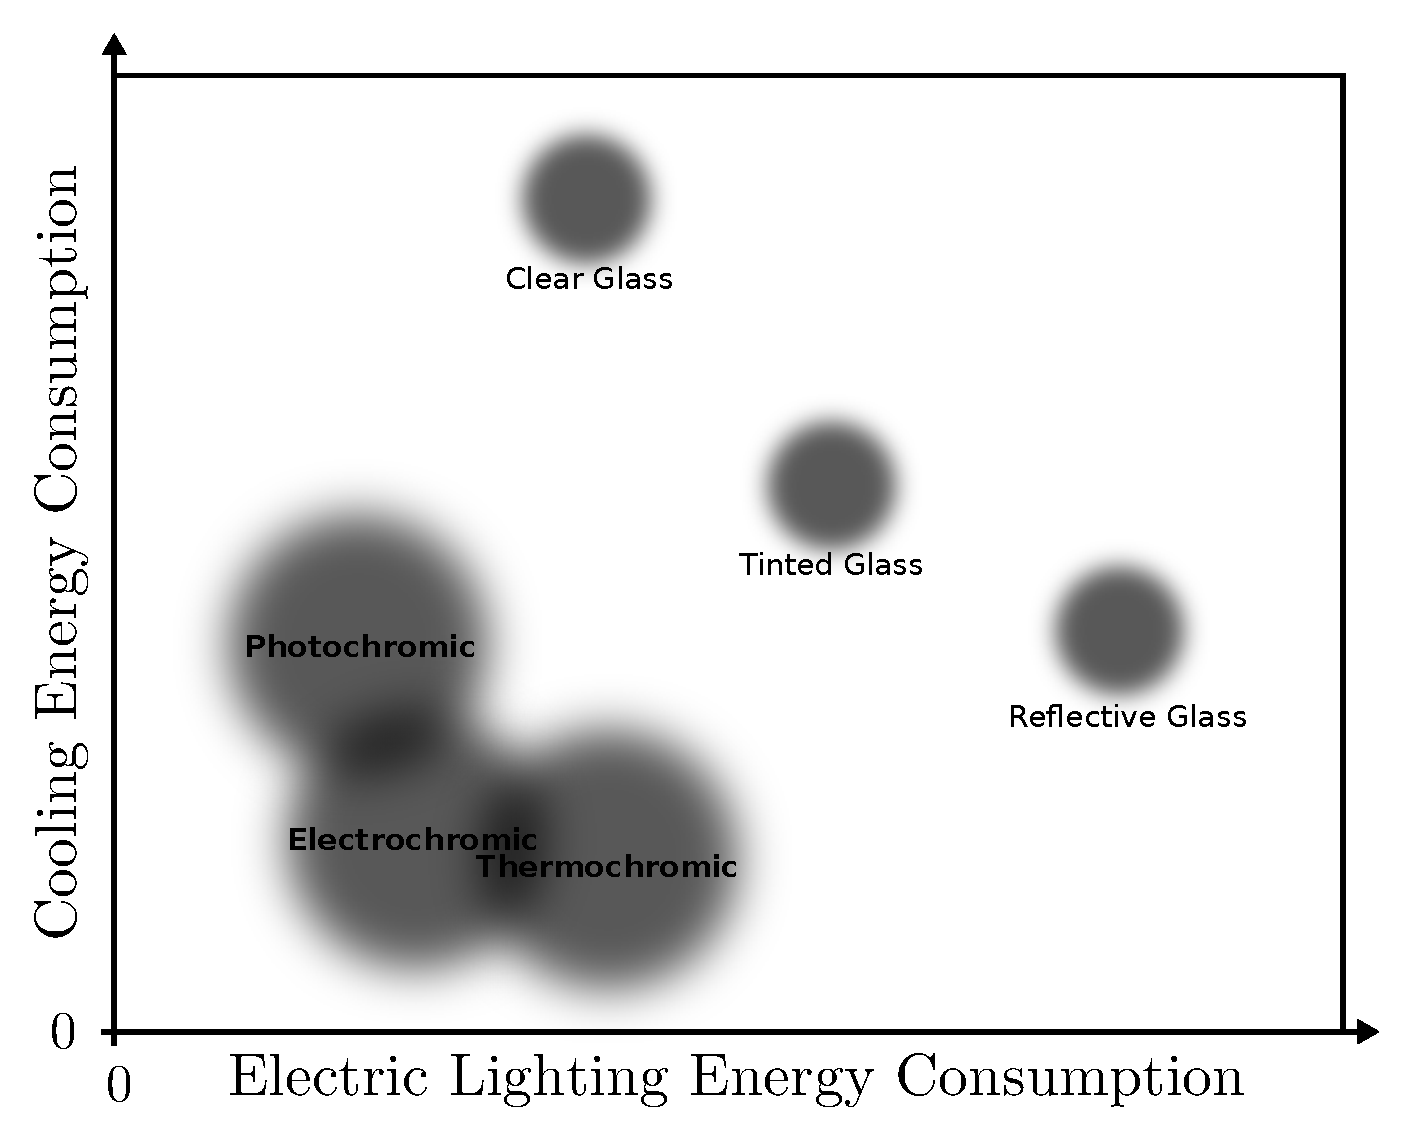
\includegraphics[width=0.5\textwidth]{Figures/chromicGlassComparison.pdf}
   \caption{Comparison of the electric lighting energy and cooling energy consumption between different
   glazing types. Adapted from (\cite{Kamalisarvestani2013},24). \textit{CHECK THIS!!: I understand
      that this graph shows the energy consumption of buildings using using different
      glazing for their windows, i.e. the window glazing impact of the building energy consumption; CHECK END.
      Also, I just drew the graph as good as I could from Kamalisarvestani2013. Is it still okay to use it?
      Should I comment on it not being exact (in case someone try to use data or something, I don't know)?}
   }
\end{figure}
%
\begin{figure}[h!]
  \centering
   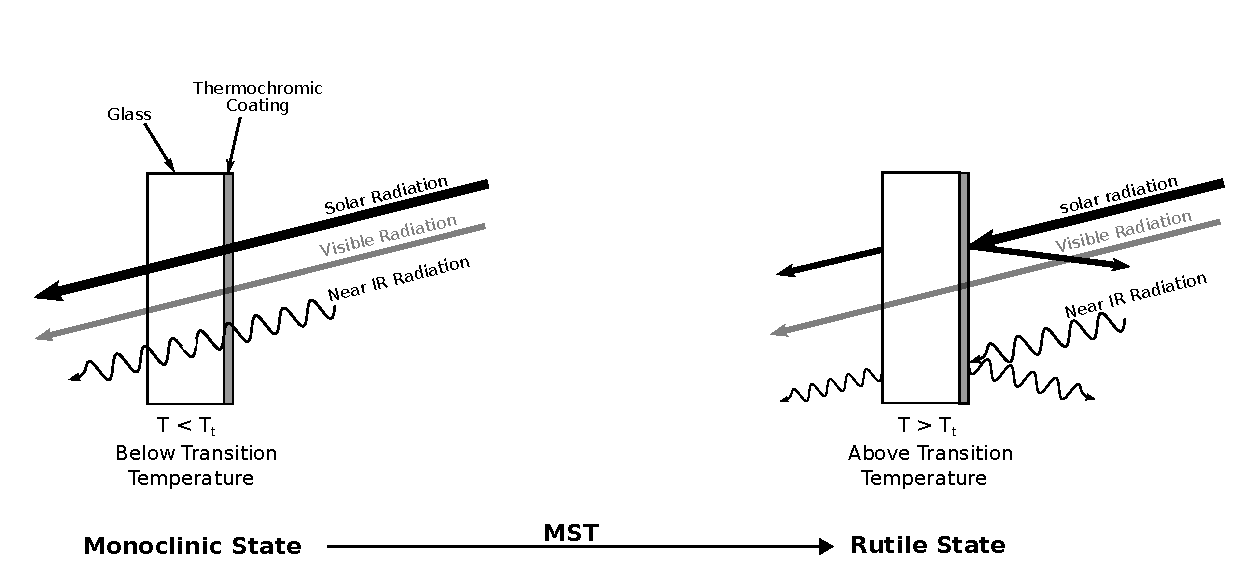
\includegraphics[width=0.9\textwidth]{Figures/TCcoating2.pdf}
   \caption{Schematic representation of thermochromic materials applied as an 
   intelligent window coating \cite{Kiria2010}.
   }
\end{figure}
%
%
\begin{figure}[h!]
  \centering
   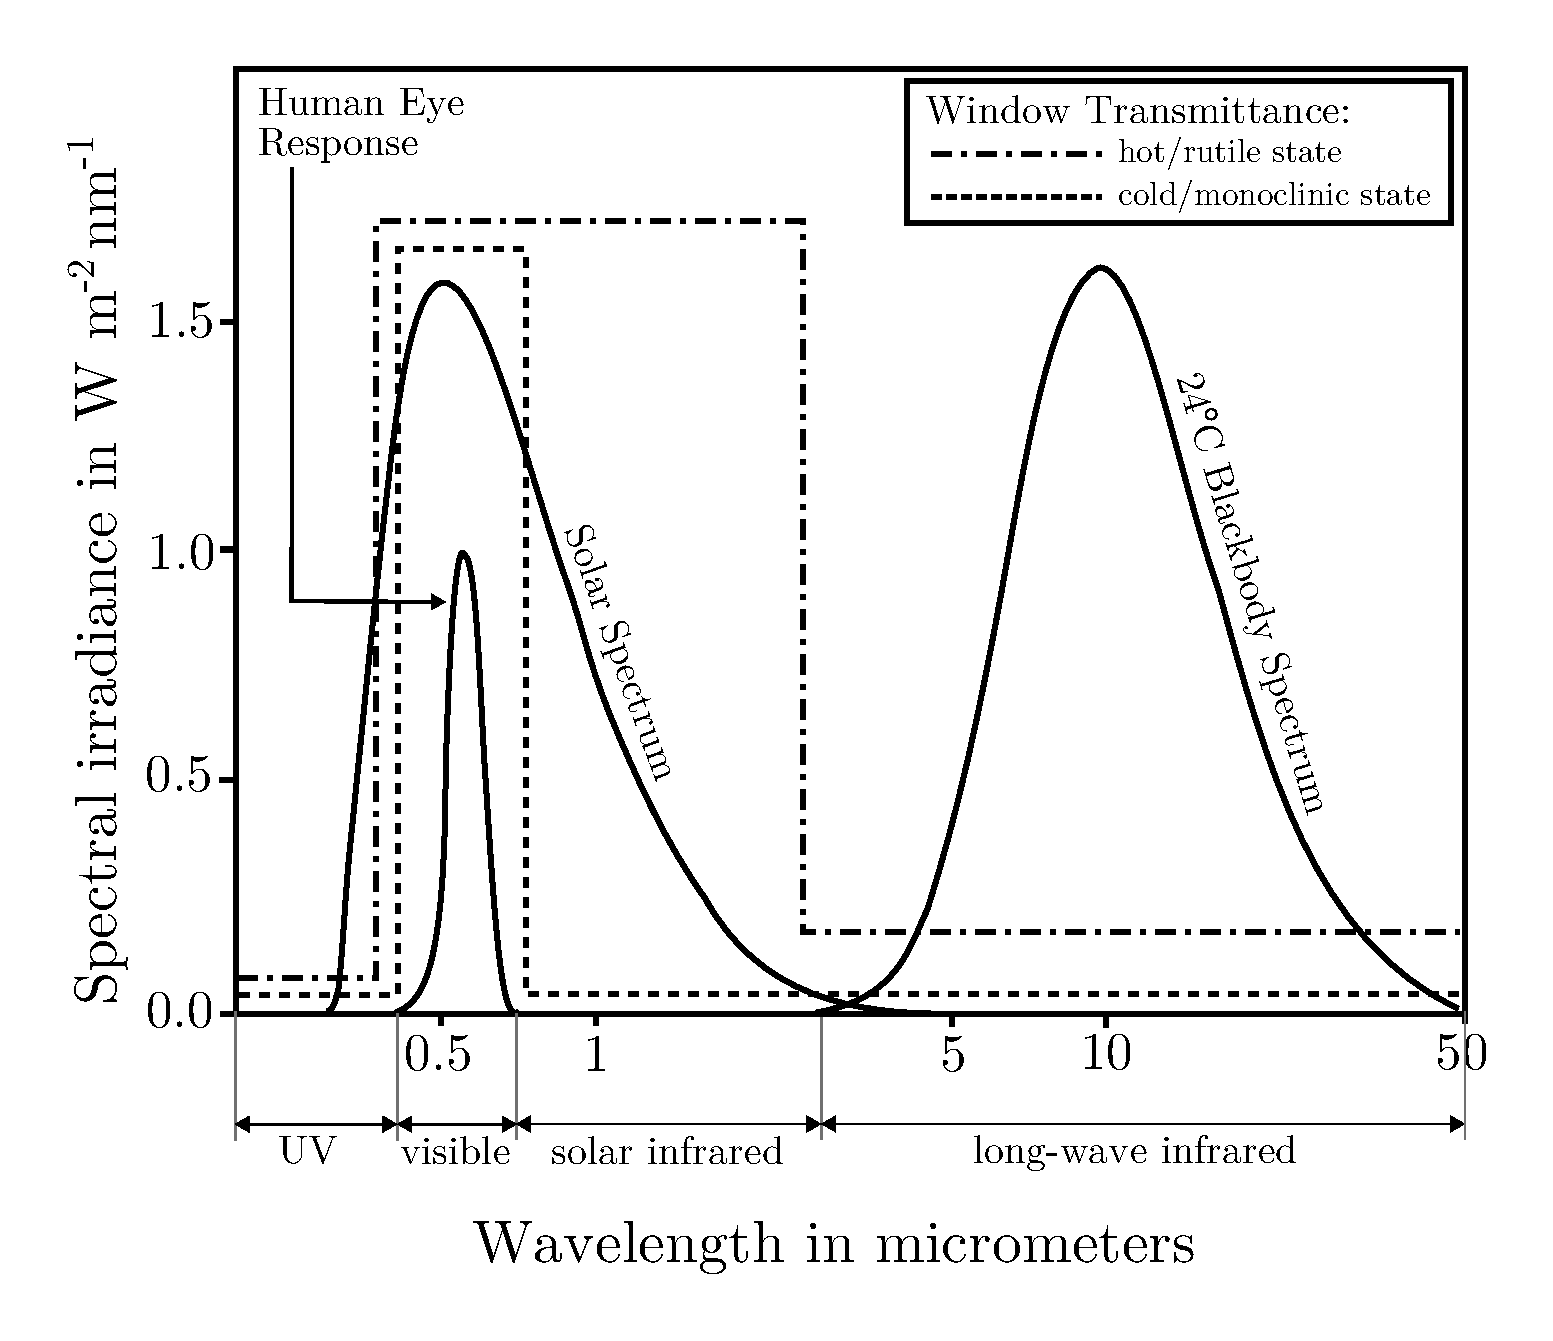
\includegraphics[width=0.5\textwidth]{Figures/TCWtransmittanceMcCluney1996andKamali2013.pdf}
   \caption{The spectral transmittance of a perfect thermochromic window, shown for both 
   cold and hot environments (the monoclinic and rutile state, repsectively). 
   Adopted from \cite{McCluney1996} \cite{Kamalisarvestani2013}
   }
\end{figure}



\textbf{Disposition:}\\
Requirements\\
- Ideal behavior- RADIATION FIGURE and PICTOGRAM\\
- ambient transition temperature\\
- 60\% transmittance in visible range, for lighting\\
-  *Doping\\
-  *Stress/strain\\
-  *thickness\\
\\
- price and mass producable: materials used and current technology\\
\\
Best Candidates:\\
(strengths and weaknesses)\\
-VO2 \\
-etc...\\


\begin{thebibliography}{9}

      \bibitem{McCluney1996}
      McCluney R, Center FSE. 
      Fenestration solar gain analysis. 
      Citeseer 1996.
      
      \bibitem{Kiri2010}
      Kiri P, Hyett G, Binions R.
      Solid state thermochromic materials.
      Advances Material Letters 2010;1(2):20.

\end{thebibliography}

\subsection{Vanadium dioxide VO$_2$; A promising candidate} \label{sec:vo2}
The most promising thermochromic material regarding thermochromic intelligent windows
is vanadium (IV) oxide.
%
%This collowing block is from blackman (along with the currents referances)
Vanadium oxide can exist in four polymorphic forms; monoclinic, rutile and two 
metastable forms (2). The metal to semiconductor phase transition from the 
monoclinic to the rutile state occurs at 68$^{\circ}$C and is fully reversble (3). 
In this transition, large changes in electrical conductivity and optical properties in the near-IR region 
occur (4), \textbf{while the change in optical region is relatively small \cite[p.~395]{Parkin2006}} . 
Above $T_t$ it behaves as a semi-metal, reflecting to a wide range of solar wavelengths
, while below, it behaves as a semiconductor, reflecting significantly less in the near infrared region 
\cite[p.~4565]{Blackman2009}.%(omskrevet av meg).
\\
\\
The transition temperature of 68$^{\circ}$C is relatively low compared other thermochromic materials.
%The most promising thermochromic material regarding thermochromic intelligent windows
%is vanadium (IV) oxide, with a relatively low transition temperature of 68$^{\circ}$C.
68$^{\circ}$C is, however, far from the comfortable temperature region around $\sim 20^{\circ}$C.
This would leave the window in its monoclinic state for all natural ambient temperatures, 
never switching it's state and leaving it unsuited as a smart coating
\cite[p.~358]{Kamalisarvestani2013} \cite[p.~39]{Kanu2010}.
%"The most promising thermochromic material for window glazing is vanadium (IV) oxide, 
% owing to its relativity low
%transition temperature of 68◦C; however, this is still not low enough for it to
%be actually used on a larger scale. The introduction of some particular dopents
%lowers the Tc to a suitable temperature". 
%\cite{Blackman2009} %(direkte sitat)
%Vanadium oxide can exist in four polymorphic forms; monoclinic VO2(M) and rutile VO2 (R) and two 
%metastable forms VO2(A) and VO2(B) (2). The monoclinic state converts to the rutile state at 68 °C 
%through a fully reversble metal to semiconductor phase transition (MST) (3). 
%In this transition, large changes in electrical conductivity and optical properties in the near-IR region 
%occur (4), and behaves as a semi-metal, reflecting to a wide range of solar wavelengths
%above $T_t$, while below it behaves as a semiconductor, reflecting 
%significantly less in the near infrared region. \cite[p.~4565]{Blackman2009} %(omskrevet av meg)
%
\\
\\
\cite{Kamalisarvestani2013}:\\
\textbf{TALK ABOUT DOPING}
(kamalisarvestani: The size and charge (84,86,87) of dopant ion, film's strain (88,89) as well as
variations in electron carrier density are the determinant factors prevailing on the fall or rise of
$T_t$ (90))
%
Many studies regarding vanadium dioxide coatings have reported low transmittance in the visible range
as discussed in the review of Kamalisarvestani et al. \cite[p.358]{Kamalisarvestani2013} and 
constitutes a the most critical weakness of VO$_2$ coatings. The switching efficiency $\eta_T$,
defined as the change in transmittance over the transition temperature $T_t$, is a measure
of the energy-saving efficieny and depends on doping (107,108), the materials microstructure (80,95,109-111)
and the film thickness (80,88) (!!!!!Also Blackman \cite[p.~4569]{Blackman2009} talk about the dependency on
thickness of VO2 films!!!! SO include this ref!!). 
The film thickness is the most important factor of the above parameters. However, because increasing 
it would reduce the transmittance of visual light, this parameter must be carefully tuned.
%
\textbf{???Important? Film thickness:}\\
For VO$_2$ the ideal film thickness regarding visual transmission
and switching efficieny is be between 40-90nm. Here the maximal
thickness should be set correspondingly to the minimum acceptable optical transmission
\cite[p.~358]{Kamalisarvestani2013} 
\cite[p.~4569]{Blackman2009}.
%And the largest changes in optical properties are seen above a critical thickness of 70 nm (14). 
The ideal film would have the maximum acceptable thickness which corresponds to the minimum 
acceptable optical transmission. In our case this is in the range 70–90 nm thick. Also
the film must be adherent and visually appealing.''

\subsection{Tungsten doping of VO$_2$ coatings} \label{sec:vo2}
The most efficient dopant of VO$_2$ coatings is the chemical element tungsten W. 
Tungsten is also known as wolfram and can be found in the periodic table
under atomic number 74. When used as a dopant in VO$_2$ it reduces the transition temperature $T_t$
of the MST and can optimally lower $T_t$ down to about $25^{\circ}$C at 2 atom \% loading
\cite[p.~4566]{Blackman2009}. 
%
There are also other problems regarding VO$_2$ coatings affecting their applicability other than $T_t$: 
vanadium dioxide have an unappealing yellow or brown color. However, this is also improved using
tungsten as a dopant and give the coating a greener/bluer color. This is depending on the relative
amount of tungsten and increases its aesthetical properties \cite[p.~4565,4569]{Blackman2009}.
%\\
%\\
%\cite[p.~4565]{Blackman2009}\\
%p.4565\\
%In addition to the practical complications of VO$_2$, it also has an unattractive color of
%yellow/brown. Luckily, the incorporation of tungsten give it a more appealing grenn/blue color,
%depending on the relative amount of tungsten.\\
%''These tech-nology advances were not transferable into commercially relevant pro-ducts 
%because of inappropriate transition temperatures, low visible light transmission, 
%unattractive visible colours and limitedfilm durability.''\\

%\cite[p.~4566]{Blackman2009}\\
%''Tungsten has been shown to be the most effective dopant ion in reducing the MST of VO2, it can optimally lower the Tc to about 25 °C at 2 atom\% loading.''
%my own words $\rightarrow$: The most effective dopant in reducing the transition temperature of 
%vanadium dioxide has shown to be tungsten, which can lower $T_t$ to about $25^{\circ}$C at
%2 atom \% loading.
%\\
%\\
%\cite[p.~4569]{Blackman2009}\\
%The film should be as thick as it can without breaking the minimum acceptable opticle transmission.
%(In the case of Blackman's study, this range were within a thickness of 70-90nm)
%In addition the film must be adherent (sticking to the surface) and visually appealing.
%\\
%\\
%p.4569 (skrevet om av meg)\\
%Using APCVD metod (reliable and reproducible) to deposit the glazing on the glass,
%they managed, by changing the ratio of vanadium precursor to water, to change the
%film apperance from powdery brown to adherent and transparent, with an improvement to greener color.
%This is accompanied by a change in film transmission in the near IR and the size of the MST 
%is dependent on the thickness of the film being above a certain level.
%Controllable doping of the films with tungsten was demonstrated. This allows control of $T_t$
%in addition to give it an attractive blue color in transmission (from tungsten), further improving the aesthetic properties.
%\\
%\\
%Seems like the figures of this paper has done experiment with VO2 using 150nm,800nm and 30nm films.
%\\
%\\
%Also, blackman mentions how the earlier work with VO2 thin films lacked control of film thickness 
%which is crucial for optimizing the optical transmission. This resulted in that even though 
%they had the required switching temperature, the excessive thickness made the 
%optical transmission too low and therefore unsuitable for application in architectural glazing. 



\newpage

%\section{Additional Theory}

\subsection{Complex permittivity and refractive index (From wikipedia) don't use, LACKING REFERENCES!}
Complex electric permittivity:
\begin{align}
   \hat{\varepsilon}_r(\omega) = \frac{\hat{\varepsilon} (\omega)}{\varepsilon_0}
\end{align}
where 
\begin{align}
   \hat{\varepsilon}_r(\omega) &= \varepsilon_r (\omega) + i\tilde{\varepsilon}_r (\omega) \\
                               &= \varepsilon_r (\omega) + i\frac{\sigma}{\omega\varepsilon_0} 
\end{align}
The complex refractive index $\hat{n}$ is given by 
\begin{align}
   \hat{n} = \sqrt{\hat{\varepsilon}_r},
\end{align}
when the magnetic properties are neglected ($\mu_r = 1$). 
From this, an expression for the complex refractive index $\hat{n} = n - \boldsymbol{i}\kappa$ can be found:
\begin{align}
   \hat{\varepsilon}_r &= \hat{n}^2 \\
   \varepsilon_r + \boldsymbol{i}\tilde{\varepsilon}_r &= (n + \boldsymbol{i} \kappa)^2 \\
   \varepsilon_r + \boldsymbol{i}\tilde{\varepsilon}_r &= n^2 - \kappa^2 + \boldsymbol{i}2n\kappa
\end{align}
giving
\begin{align}
   \varepsilon_r &= n^2 - \kappa^2     &\tilde{\varepsilon}_r  &= 2n\kappa.
\end{align}
Taking the absolute value or modulus of the relative permettivity
\begin{align}
   |\hat{\varepsilon}_r| &= \sqrt{ \varepsilon_r^2 + \tilde{\varepsilon}_r^2} \\
   |\hat{\varepsilon}_r| &= \sqrt{ (n^2 - \kappa^2)^2 + (2n\kappa)^2} \\
   |\hat{\varepsilon}_r|^2 &= (n^4 - 2n^2\kappa^2 + \kappa^4) + 4n^2\kappa^2 \\
   |\hat{\varepsilon}_r|^2 &= n^4 + 2n^2\kappa^2 + \kappa^4 \\
   |\hat{\varepsilon}_r|^2 &= (n^2 + \kappa^2)^2 \\
   |\hat{\varepsilon}_r| &= n^2 + \kappa^2 
\end{align}
and adding or substracting the real part of the permittivity, gives
\begin{align}
   |\hat{\varepsilon}_r| + \varepsilon_r &= (n^2 + \kappa^2) + (n^2 - \kappa^2) = 2n^2\\
   |\hat{\varepsilon}_r| - \varepsilon_r &= (n^2 + \kappa^2) - (n^2 - \kappa^2) = 2\kappa^2.
\end{align}
Refomulating the expression gives the real and imaginary parts of $\hat{n}$
\begin{align}
   n      &= \sqrt{ \frac{|\hat{\varepsilon}_r| + \varepsilon_r}{2}} 
           = \sqrt{ \frac{|\hat{\varepsilon}| + \varepsilon}{2\varepsilon_0}}\\
   \kappa &= \sqrt{ \frac{|\hat{\varepsilon}_r| - \varepsilon_r}{2}} 
           = \sqrt{ \frac{|\hat{\varepsilon}| - \varepsilon}{2\varepsilon_0}}
\end{align}


\subsection{Polarizability. Don't use, LACKING REFERENCES}
When a neutral atom is placed in an electric field $\boldsymbol{E}$, the field tries to rip the
atom apart by pushing the nucleus in the direction of the field and the electrons in the opposite direction.
Because of the attraction between the positive and negative charge within the atom, an equilibrium displacement
of the electrons compared to the nucleus is achieved, leaving the atom polarized and giving it a
dipole moment. The dipole moment can be approximated by
\begin{align}
   \boldsymbol{p} = \alpha \boldsymbol{E},
\end{align}
where $\alpha$ is the atomic polarizability and may depend on the detailed structure of the atom.
For more complicated situations, like an asymmetrical molecule, the gained dipole moment of the 
molecule does not necessarily have to be in the same direction as the applied electric field.
In such a case, the scalar polarizability in the expression above is replaced by a polarizability tensor
\begin{align}
   \boldsymbol{\alpha} = 
\begin{bmatrix}
   \alpha_{xx}   &   \alpha_{xy}  &  \alpha_{xz}  \\
   \alpha_{yx}   &   \alpha_{yy}  &  \alpha_{yz}  \\
   \alpha_{zx}   &   \alpha_{zy}  &  \alpha_{zz} 
\end{bmatrix}
.
\end{align}
In this way, an applied eletric field induces many dipole moments in a material. In addition,
any polar molecules will be subject to a torque, aligning it to the direction of the field.
These two mechanisms leads to the polarization $\boldsymbol{P}$ of the material
\begin{align}
   \boldsymbol{P} = \text{dipole moment per unit volume} = \varepsilon_0 \chi_e \boldsymbol{E}.
\end{align}
In the above expression, there has been assumed a linear dielectric media, where $\chi_e$ is the electric 
susceptibility and depends on the microscopic structure of the material, in addition to the external 
temperature (\cite{Griffiths},p.160-166, 179)

\subsection{The electric potential, Laplace's equation and the Uniqueness Theorem}
The usual task of electrostatics is to ompute the electric field $\boldsymbol{E}$ given a 
stationary charge distribution $\rho{\boldsymbol{r}}$
\begin{align}
   \boldsymbol{E}(\boldsymbol{r}) 
   &= \frac{1}{4 \pi \varepsilon_0} \int \frac{\boldsymbol{\hat{d}}(\boldsymbol{r'})}
                                              {d(\boldsymbol{r'})^2} 
                                                            \rho(\boldsymbol{r'}) d\!\boldsymbol{r'} 
                                                            \\
   &= \frac{1}{4 \pi \varepsilon_0} \int \frac{\boldsymbol{r} - \boldsymbol{r'}}
                                              {\big|\boldsymbol{r} - \boldsymbol{r'}\big|^3} 
                                                           \rho(\boldsymbol{r'}) d\!\boldsymbol{r'}.
\end{align}
However, it is usually simpler to calculate the potential
\begin{align}
   \label{electricPotential}
   V(\boldsymbol{r}) 
   &= \frac{1}{4 \pi \varepsilon_0} \int \frac{1}{\big|\boldsymbol{r} - \boldsymbol{r'}\big|} 
                                                           \rho(\boldsymbol{r'}) d\!\boldsymbol{r'}
\end{align}
first and then calculate the electric field from
\begin{align}
   \boldsymbol{E} = - \nabla V.
\end{align}
This might in some situations, where do do not necessarily know $\rho$ but only the total amount of 
charge, also be to tough to handle analytically. In situations like these it is better to use
Poisson's equation
\begin{align}
   \label{poisson}
   \nabla^2 V= - \frac{1}{\varepsilon_o} \rho,
\end{align}
which together with appropriate boundary conditions, is equivalent to Eq.\eqref{electricPotential}.
Very often, we are interested in finding the potential containing no charge (because the charge is 
located on the outside of our region of interest. In such cases Eq. \eqref{poisson} reduces to
Laplace's equation (\cite{Griffiths}, p.110-111)
\begin{align}
   \label{laplace}
   \nabla^2 V = 0.
\end{align}
According to the \textit{Uniqueness Theorems}, the solution to Laplace's equation is uniquely 
determined in some volume if the potential is specified on the boundary of the volume. This
easily extends to Poisson's equation by further requiring, in addition to the 
potential on the boundary, that the charge distribution throughout the region is known.
\\
\\
When considering conductors, charge are allowed to move freely and  might start to rearrange themselves,
leading to the \textit{Second uniqueness theorem}, which states that the potential in a given volume,
surrounded by conductors is uniquely determined if the total charge on each conductor is given.
\\
\\
The uniqueness theorem grants an enlarged mathematical freedom in the approach of finding the potential
of a region of space. This is because the boundary uniquely determines the potential in the region enclosed
region and any approach giving the correct boundary conditions would give you the correct potential 
function through Laplace's equation Eq. \eqref{laplace}. This allows the use of tricks, like for example
the classical \textit{method of images} (\cite{Griffiths}, p.116-121).
%SOME EXTRA STUFF:
%\textbf{D'Alembert Operator $\square$}
%\begin{align*}
  %\square  &= \partial ^{\mu} \partial _{\mu}
   %\\
           %&= \frac{1}{c^2} \frac{\partial ^2}{\partial t^2} 
               %- \frac{\partial ^2}{\partial x^2} 
               %- \frac{\partial ^2}{\partial y^2} 
               %- \frac{\partial ^2}{\partial z^2} 
   %\\
           %&= \frac{1}{c^2} \frac{\partial ^2}{\partial t^2} - \nabla ^2
%\end{align*}

%\textbf{Lorentz Gauge:} \\
%For Lorentz invariance, convenient to choose the Lorenz gauge:
%\begin{align*}
   %\square \vec{A} = \Bigg[ \frac{1}{c^2} \frac{\partial ^2}{\partial t^2} - \nabla ^2 \Bigg] \vec{A} = \mu_0 \vec{J}
%\end{align*}
%\begin{align*}
   %\square \phi = \Bigg[ \frac{1}{c^2} \frac{\partial ^2}{\partial t^2} - \nabla ^2 \Bigg] \phi = \frac{\rho}{\epsilon _0}
%\end{align*}
 %moved to notes
%\section{Basic Theory}
\subsection{The electric potential, Laplace's equation and the Uniqueness Theorem}
The usual task of electrostatics is to compute the electric field $\boldsymbol{E}$ given a 
stationary electric charge distribution $\rho_E{\boldsymbol{r'}}$
\begin{align}
   \label{electricField}
   \boldsymbol{E}(\boldsymbol{r}) 
   %&= \frac{1}{4 \pi \varepsilon_0} \int \frac{\boldsymbol{\hat{d}}(\boldsymbol{r'})}
                                              %{d(\boldsymbol{r'})^2} 
                                                            %\rho(\boldsymbol{r'}) d\!\boldsymbol{r'} 
                                                            %\\
   &= \frac{1}{4 \pi \varepsilon_0} \int \frac{\boldsymbol{r} - \boldsymbol{r'}}
                                              {\big|\boldsymbol{r} - \boldsymbol{r'}\big|^3} 
                                                           \rho(\boldsymbol{r'}) d\!\boldsymbol{r'}.
\end{align}
The notation for Eq.\eqref{electricField} can be shown in Figure \ref{fig:electricField}
and $\varepsilon_0 = 8.85 \cdot 10 ^{-12} \text{C}^2/\text{Nm}^2$ is the permittivity of free space
\cite[.~58-62]{Griffiths}.
%
\begin{figure}[h!]
  \centering
   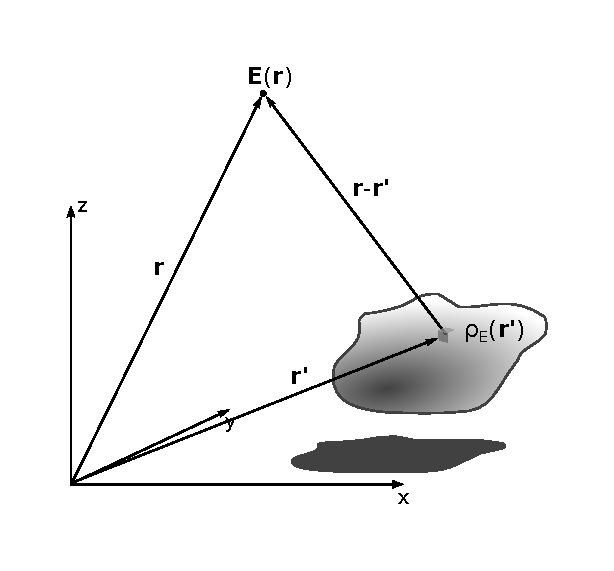
\includegraphics[width=0.5\textwidth]{../Figures/electricFieldcoord.pdf}
   \caption{
      The electric field $\boldsymbol E (\boldsymbol r)$ (at position $\boldsymbol r$)
      due to the charge distribution $\rho_E$ located at $\boldsymbol{r'}$.
   }
   \label{fig:electricField}
\end{figure}
%
However, it is usually simpler to calculate the electric potential $\Psi$
\begin{align}
   \label{electricPotential}
   \Psi(\boldsymbol{r}) 
   &= \frac{1}{4 \pi \varepsilon_0} \int \frac{1}{\big|\boldsymbol{r} - \boldsymbol{r'}\big|} 
                                                           \rho(\boldsymbol{r'}) d\!\boldsymbol{r'}
\end{align}
first and then calculate the electric field from
\begin{align}
   \boldsymbol{E} = - \nabla \Psi.
\end{align}
This might in some situations, where do do not necessarily know $\rho$ but only the total amount of 
charge, also be to tough to handle analytically. In situations like these it is better to use
Poisson's equation
\begin{align}
   \label{poisson}
   \nabla^2 \Psi= - \frac{1}{\varepsilon_o} \rho,
\end{align}
which together with appropriate boundary conditions, is equivalent to Eq.\eqref{electricPotential}.
Very often, we are interested in finding the potential containing no charge (because the charge is 
located on the outside of our region of interest. In such cases Eq. \eqref{poisson} reduces to
Laplace's equation (\cite{Griffiths}, p.110-111)
\begin{align}
   \label{laplace}
   \nabla^2 \Psi = 0.
\end{align}
According to the \textit{Uniqueness Theorems}, the solution to Laplace's equation is uniquely 
determined in some volume if the potential is specified on the boundary of the volume. This
easily extends to Poisson's equation by further requiring, in addition to the 
potential on the boundary, that the charge distribution throughout the region is known.
\\
\\
When considering conductors, charge are allowed to move freely and  might start to rearrange themselves,
leading to the \textit{Second uniqueness theorem}, which states that the potential in a given volume,
surrounded by conductors is uniquely determined if the total charge on each conductor is given.
\\
\\
The uniqueness theorem grants an enlarged mathematical freedom in the approach of finding the potential
of a region of space. This is because the boundary uniquely determines the potential in the region enclosed
region and any approach giving the correct boundary conditions would give you the correct potential 
function through Laplace's equation Eq. \eqref{laplace}. This allows the use of tricks, like for example
the classical \textit{method of images} (\cite{Griffiths}, p.116-121).





\subsection{Polarizability}
When a neutral atom is placed in an electric field $\boldsymbol{E}$, the field tries to rip the
atom apart by pushing the nucleus in the direction of the field and the electrons in the opposite direction.
Because of the attraction between the positive and negative charge within the atom, an equilibrium displacement
of the electrons compared to the nucleus is achieved, leaving the atom polarized and giving it a
dipole moment. The dipole moment can be approximated by
\begin{align}
   \boldsymbol{p} = \alpha \boldsymbol{E},
\end{align}
where $\alpha$ is the atomic polarizability and may depend on the detailed structure of the atom.
For more complicated situations, like an asymmetrical molecule, the gained dipole moment of the 
molecule does not necessarily have to be in the same direction as the applied electric field.
In such a case, the scalar polarizability in the expression above is replaced by a polarizability tensor
\begin{align}
   \boldsymbol{\alpha} = 
\begin{bmatrix}
   \alpha_{xx}   &   \alpha_{xy}  &  \alpha_{xz}  \\
   \alpha_{yx}   &   \alpha_{yy}  &  \alpha_{yz}  \\
   \alpha_{zx}   &   \alpha_{zy}  &  \alpha_{zz} 
\end{bmatrix}
.
\end{align}
In this way, an applied eletric field induces many dipole moments in a material. In addition,
any polar molecules will be subject to a torque, aligning it to the direction of the field.
These two mechanisms leads to the polarization $\boldsymbol{P}$ of the material
\begin{align}
   \boldsymbol{P} = \text{dipole moment per unit volume} = \varepsilon_0 \chi_e \boldsymbol{E}.
\end{align}
In the above expression, there has been assumed a linear dielectric media, where $\chi_e$ is the electric 
susceptibility and depends on the microscopic structure of the material, in addition to the external 
temperature (\cite{Griffiths},p.160-166, 179)



\subsection{Plasmons}

\subsection{\textbf{The Drude model} \cite{Hofmann} }
Defining the differences between the electrical properties of metals, semiconductors and insulators
is not a trivial matter. To put it simple, metals are good conductors, while semiconductors and 
insulators are not. However, semiconductors such as silicon conduct electrisity relatively well,
so the picture is not quite that simple.
\\
\\
A simple model, with fundamental importance regarding electrical conductivity, was suggested by
P. Drude in an attempt to explain the observed properties of metals. It is assumed that the 
electrons in a solid behave like a classical gas and do not interact with each other whatsoever.
Coloumb interaction is also neglected. This is known as the \textit{independent electron approximation}. 
The electron gas can be viewed as negatively charged particles bouncing about
immobile immobile positively charged ion cores. The only form of interaction in this model
are instantaneous collision between the electrons and ions; see Figure \ref{fig:DrudeModel}. 
The simplification of removing the Coloumb ion-electron interaction is called the 
\textit{free electron approximation}
%
\begin{figure}[h!]
  \centering
   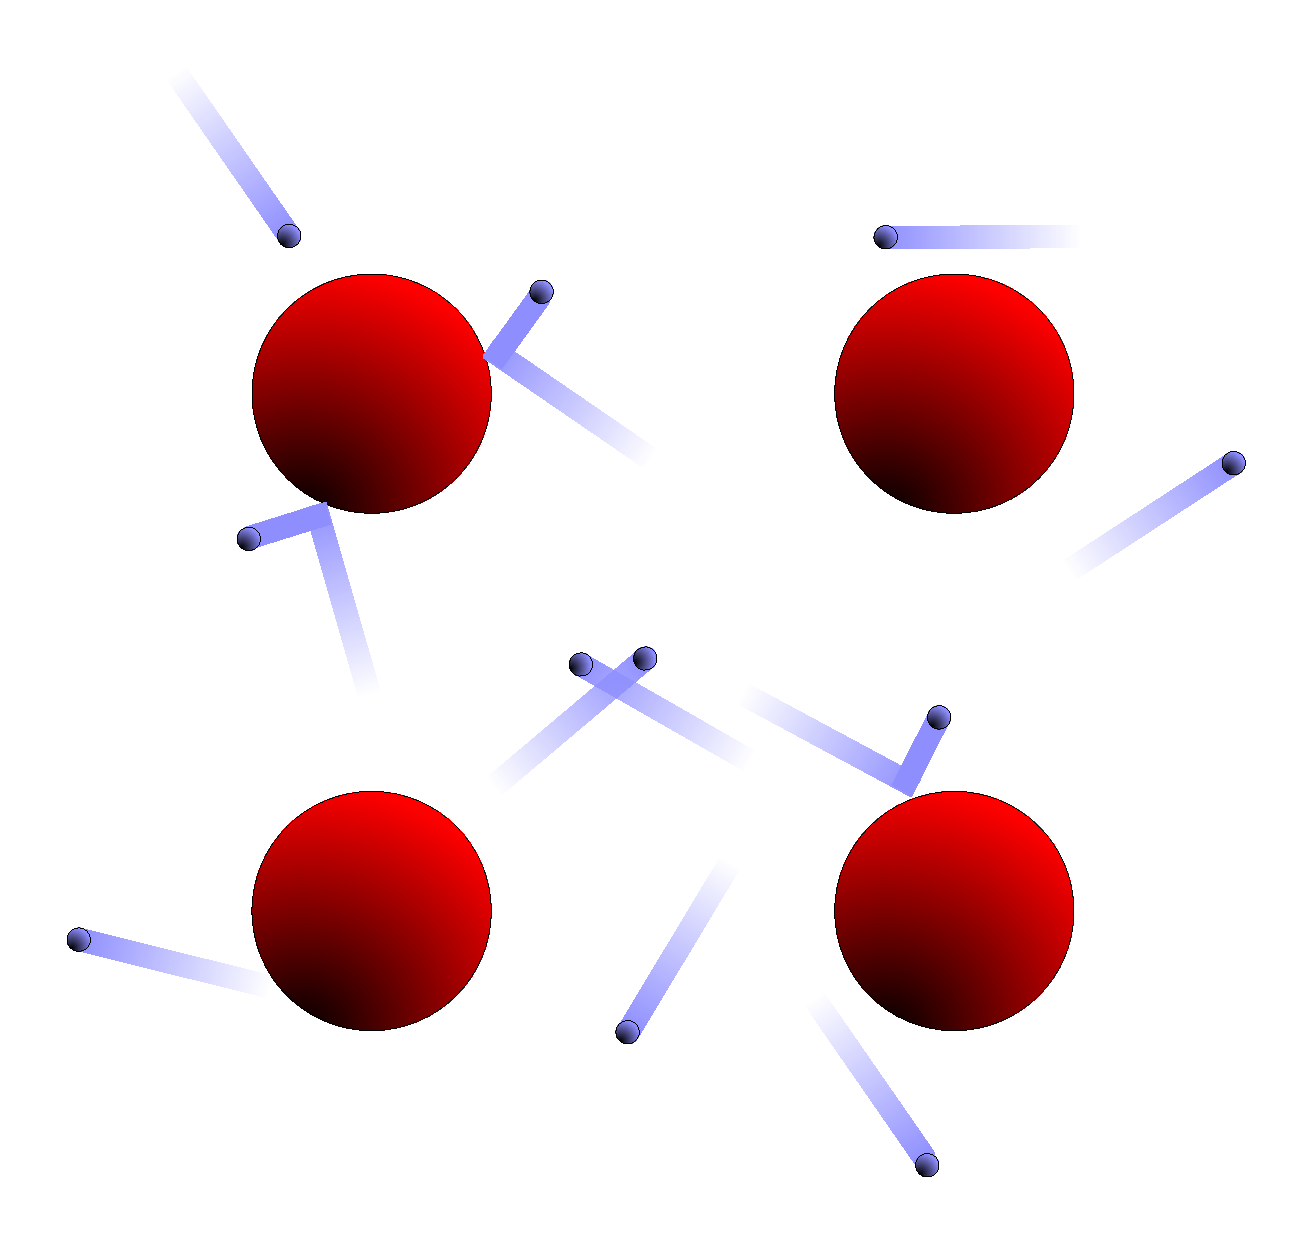
\includegraphics[width=0.5\textwidth]{../Figures/DrudeModel.pdf}
   \caption{ 
      The Drude model. A non-interacting electron gas (blue) is swirling around and colliding with 
      stationary positive ion cores (red). 
      Since all Coloumb forces are neglected together with electron-electron
      collsion, this ion-electron interaction is the only one being considered.
   }
   \label{fig:DrudeModel}
\end{figure}
%
The electrons reach thermal equilibrium with the lattice through the collisions, giving them
the kinetic energy:
\begin{align}
   \frac{1}{2}m_e v_t = \frac{3}{2}k_B T.
\end{align}
The average time between two collisions is called the relaxation time $\tau$, with the 
corresponding mean free path defined as $\lambda  = \tau v_t$. The probability for a 
electron to collide per unit time is assumed to be $1/\tau$. 
\\
\\
It is necessary to determine the conduction electron density $\rho_{c,e}$ in order to describe
properties such as electrical conductance. Assuming that every atom contributes 
every electron in its outermost shell $N_e$, e.g. that alkali metals contribute $N_e = 1$ and 
that earch alkaline earth metals contribute $N_e = 2$ etc. The number of atoms $N_a = \rho_m /m_a$, 
where $\rho_m$ is the density of the metal in [kg/m$^{-3}$] and $m_a$ is the atomic mass in [kg] 
(mass per atom).

\subsection{Conductivity; the Drude model}
Subjecting the drude metal of an electric field $\boldsymbol E$ will lead to a drift of the electrons
\begin{align}
   \frac{d \boldsymbol v}{dt} m_e = -e \boldsymbol E ,
\end{align}
where $e$ is the elementary charge. The solution is given by
\begin{align}
   \boldsymbol v (t) = \frac{-e \boldsymbol E t}{m_e}.
\end{align}
Assuming that the drift montion is destroyed in a collision, the average drift speed 
of the electrons become
\begin{align}
   \bar{\boldsymbol v }(t) = \frac{-e \boldsymbol E \tau}{m_e},
\end{align}
which is very slow compared to the thermal movement of the electrons $v_t$.
\\
\\
Considering an area $A$ perpendicular to the electric field, the amount of charge passing through 
the area is $-e n_e | \bar{\boldsymbol v} | A $ and the resulting current density would be
\begin{align}
   \boldsymbol j = n  \bar{\boldsymbol v} (-e) = \frac{n_e e^2 \tau}{m_e} \boldsymbol E \equiv \sigma \boldsymbol E = \boldsymbol E / \rho.
\end{align}
This is the familiar Ohm's law, with the conductivity 
\begin{align}
\sigma = \frac{n_e e^2 \tau}{m_e}
\end{align}
and the resistivity $\rho$. The $e^2$ dependence comes from the size of the pulling force
due to the electric field, i.e. how fast the particles move, and the other is how the same
charge, now moving, defines the current. This also means that we would get the same 
result for carriers with charge $e$ instead of $-e$, which would be the case for semiconductors
with positive holes.

\subsection{Optical reflectivity of drude metals}
The optical properties of materials are described by the complex refractive index $N(\omega)$ or 
the dielectric constant $\varepsilon(\omega)$. 
To explain the reflectivity of metals we can concider an electron in an electromagnetic 
field induced by an optical incident wave with wavenumber $q = 2\pi N/\lambda_0$, where 
$\lambda_0$ is the wavelength of the wave in free space.\\
If $\omega$ is low, we basically retain the DC behavior. However, if $\omega$ is so high that 
$1/\omega \ll \tau$, the electrons does not manage to react fast enough and the collisions with 
the ions altogether can be ignored (this is fulfilled for optical frequencies when $\tau=10^{-14}$s). 
The electrons can now be treated as completely free, and a single electron follows
\begin{align}
   m_e \frac{d^2x(t)}{dt^2} = -e E(t) = -e E e^{-i \omega t}.
   \label{freeElectronGas}
\end{align}
A good ansatz for the solution is setting $x(t) = xe^{-i \omega t}$, which mean that 
the electron is oscillating along with the electric field. This gives an amplitude of
\begin{align}
   x = \frac{eR}{m_e \omega^2}.
\end{align}
The corresponding polarization due to the dipole moment of $-ex$ for a solid with conduction electron
density $n_e$ is
\begin{align}
   P = -n_e ex = -\frac{n_e e^2E}{m_e \omega^2}.
\end{align}
From the constitutive relation
\begin{align}
   D = \varepsilon \varepsilon_0 E = \varepsilon_0 E + P,
\end{align}
we get that 
\begin{align}
   \varepsilon = 1 + \frac{P}{\varepsilon_0 E} = 1 - \frac{n_e e^2}{\varepsilon m_e \omega^2}
   \equiv 1 - frac{\omega_p^2}{\omega^2},
\end{align}
with the plasma frequency $\omega_p$ defined as
\begin{align}
   \omega_p = \frac{n_e e^2}{m_e\varepsilon_0}.
\end{align}
We can distinguish between two different cases and resulting outcome can
be seen from the the electromagnetic plane wave
\begin{align}
   \boldsymbol E (z,t) = \boldsymbol E_0 e^{i(2\pi N z/ \lambda_0 - \omega t)}.
\end{align}
In case 1) $\omega < \omega_p$ 
and $\varepsilon$ is a real and negative, $\varepsilon = \Re\{\varepsilon\} < 0$.
Therefore, $N = \sqrt{\varepsilon}$ is purely imaginary, and the wave penetrating the solid
is exponentially damped. Because Eq.\eqref{freeElectronGas} contain no inelastic properties, nothing
is absorbed. The light that is not transmitted into the medium must therefore, due to energy conservation, be
reflected back. 
For $\omega > \omega_p$, the dielectric constant is real and positive ,$\varepsilon = \Re\{\varepsilon\} > 0$,
and so is, followingly, the index of refraction. The result is a plane wave that propagates 
into the metal. This explains why metals are so reflective, or shiny. They are reflective for 
low-frequency light, but transparent for high-frequency light. The transition happens
at the plasma frequeny, which can be calculated solely from the conduction electron density of 
the metal. For most metals, the plasma frequency is in the far UV region, making them reflective 
in the visible range. Frequently, the plasma energy $\hbar \omega_p$ is used instead of the plasma frequency
$\omega_p$.

\subsection{Shortcomings of the Drude model}
The quenstionable assumptions of the Drude model is the removal of the electron-electron interaction
together with all the Coloumb forces. In addition, the assumption of treating the electrons as 
particles is not justified due to the fact that their de Broglie wavelength, in the case of thermal
electrons, is in the order of nanometers. The assumption would however only satisfy electrons moving
in structures much larger than the de Broglie wavelength.
\\
\\
The resulting conductivity of the model is not high enough at low temperatures, and is due to the
assumption of a fixed mean free path, given by the atomic spacing. Apparantly, at low temperature,
the electrons manage to sneak past the other electrons and ions. 
\\
\\
Also, the conductivity of alloys, in which impurities drastically reduce the conductivity, finds no
justification in the Drude model. 


\subsection{\textbf{Dielectrics}}
\subsection{Microscopic polarization}
There are several mechanismc causing microscopic electric dipole moments that lead to macroscopic 
polarization. E.g. displacement of electronic clouds and core, opposite displacement of the ions 
in a solid or
orientation of permanent dipoles such as water molecules, called orientational polarization.

\subsection{The local field}
To calculate the microscopic polarizability $\alpha$ of the atoms making up the solid, start with
the constitutive relation and assume that $\boldsymbol P$ can be written as the total dipole moment 
per unit volume
\begin{align}
   \boldsymbol P = (\varepsilon - 1 ) \varepsilon_0 \boldsymbol E = \frac{N}{V} \boldsymbol p = \frac{N}{V}\alpha \boldsymbol E.
   \label{nonLocalP}
\end{align}
Because a microscopic dipole within the solid does not simply feel the average electric field 
$\boldsymbol E$ but a microscopic local and stronger electric field $\boldsymbol E_{loc}$, the polarizability
can bot be correctly calculated from the above expression.
Without derivation, the approximate local field can be given by
\begin{align}
   \boldsymbol E_{loc} = \frac{1}{3}(\varepsilon + 2) \boldsymbol E.
\end{align}
So, with
\begin{align}
   \boldsymbol P = \frac{N}{V}\alpha \boldsymbol E_{loc}
\end{align}
and approximating the polarization $\boldsymbol P$ with Eq.\eqref{nonLocalP}, 
we get the so-called Clausius-Mossotti relation
\begin{align}
   \alpha = \frac{\varepsilon - 1}{\varepsilon + 2} \frac{3 \varepsilon_0 V}{N},
\end{align}
relating the atomic polarizabiliy to the dielectric constant.

\subsection{Frequency dependence of the dielectric constant}
The frequency dependent permittivity  $\varepsilon (\omega)$ is usually called the dielectric function.
For insulators, $\varepsilon(\omega)$ is complex and energy can be resonantly transferred to the solid
for certain frequencies. $\varepsilon(\omega)$ implies a frequency dependence of the refractive
index $N(\omega)$. Most of the frequency dependence can be explained by a simple idea 
combined with knowledge about the polarization mechanisms and how the different polarization mechanisms
manages to keep up with the oscillating electric field. E.g. orientation polarization and ionic polarization
does not manage to oscillate fast enough at higher frequencies, while the atomic polarization will, see
Figure \ref{fig:polarizationContribution}.
%
\begin{figure}[h!]
  \centering
   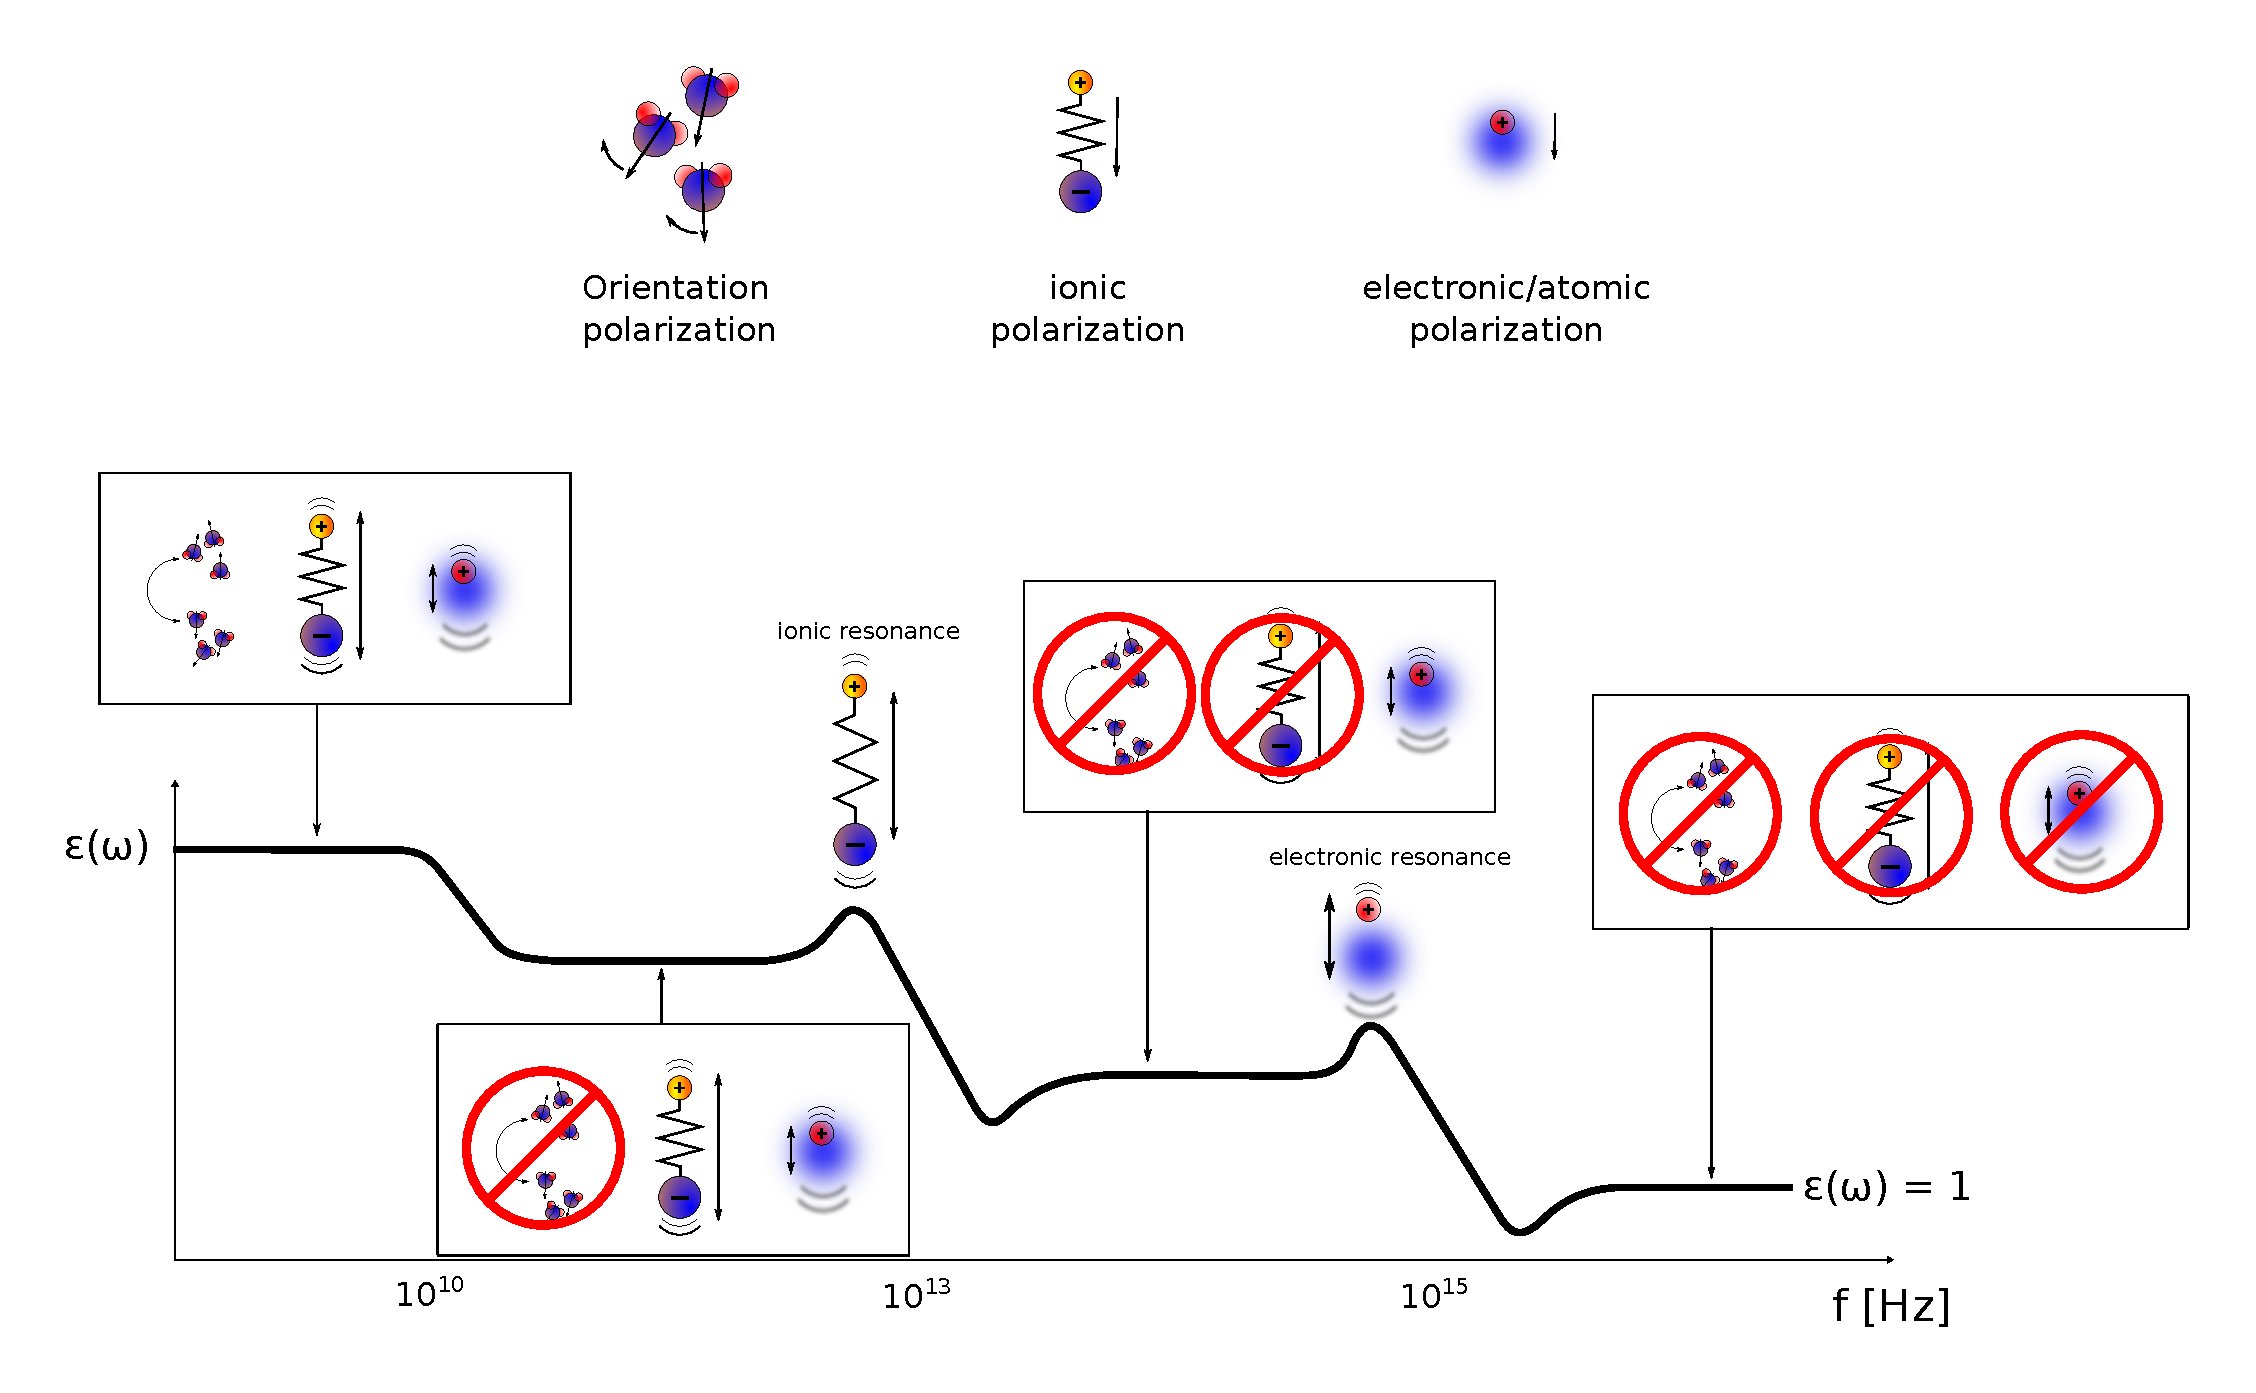
\includegraphics[width=1.0\textwidth]{../Figures/polarizationContributionToPermittivity.pdf}
   \caption{ 
      The contribution of orientation, ionic and electronic polarization. As the frequency
      of the applied electric field increases, the different polarization mechanisms fail to remain in 
      step with the field when above a characteristic frequency. At sufficiently high 
      frequencies the material no longer manages to polarize and the dielectric constant drops 
      to 1, corresponding to the permittivity of free space. Figure is adapted from 
      \cite{cambdridgePermittivityPage}.
   }
   \label{fig:polarizationContribution}
\end{figure}
%
\\
\\
For a quntitative description of the frequencydependence of $\varepsilon$ we can consider a simplified
version of ionic vibration.
Light can couple to optical phonons, e.g in ionic crystals where the phonons correspond to
an out-of-phase virbation of the positive and negative ions in the unit cell. 
These vibrations can be approximated by independent harmonic oscillators driven by an electric field
$E ^{-i\omega t}$, with one such oscillator per unit cell of the crystal. Each oscillator have a 
resonant frequency of $\omega_o = (2\gamma/M)^{1/2}$, where $\gamma$ is the force constant and
$M$ is the reduced mass of the two ions. The motion is damped by a term proportional to the velocity
$\eta d\!x\!/\!d\!t$ and represents the excitation of other vibrations in the material,
due to the large displacement. 
The resulting equation of motion is that of a driven harmonic oscillator with damping
\begin{align}
   \frac{d^2x}{dt^2} + \eta \frac{dx}{dt} + \omega_0^2 x = \frac{eE}{M}e^{-i\omega t}.
\end{align}
A good ansatz for the solution is 
\begin{align}
   x(t) = Ae^{-i \omega t},
\end{align}
resulting in the amplitude
\begin{align}
   A &= \frac{eE}{M} \frac{1}{\omega_0^2 - \omega^2 - i \eta \omega}  \\
     &=  \frac{eE}{M} \Bigg[ \frac{\omega_0^2 - \omega^2}{(\omega_0^2 - \omega^2)^2 +\eta^2 \omega^2} 
+ \frac{i\eta \omega}{(\omega_0^2 - \omega^2)^2 + \eta^2 \omega^2} \Bigg]
\end{align}
Using this as the ionic vibration, we can calculate the total polarization for a crystal with
$N$ unit cells and volume V. Considering only one type of ions with a density $N/V$ and effective
atomic polarizability $\alpha$, assuming both ionic and atomic polarization, $P_i(\omega)$, $P_a(\omega)$,
the result reads
\begin{align}
   P(\omega) = P_i(\omega) + P_a(\omega) = \frac{N}{V}eA(\omega)e^{-i \omega t} + \frac{N}{V}\alpha E e^{-i \omega t}.
\end{align}
When dealing with two types of ions like in a NaCl crystal, the different polarizabilities can be
taken care of by a suitable definition of $\alpha$. The resulting dielectric function can be calculated
from
\begin{align}
   \varepsilon_0 \varepsilon (\omega) E(\omega) = P(\omega) + \varepsilon_0 E(\omega),
\end{align}
giving
\begin{align}
   \varepsilon (\omega) &= \frac{P(\omega)}{\varepsilon_0 E e^{-i \omega t}} + 1  \\
                        &= \frac{NeA(\omega)}{V\varepsilon_0} + \frac{N \alpha}{V \varepsilon_0} + 1 \\
                        &= \frac{NeA(\omega)}{V\varepsilon_0} + \varepsilon\!_{_{opt}}.
\end{align}
Here, $\varepsilon_{opt}$ is the high frequency or optical limit, where the fields move to quickly for the 
ions to respond and $P_i(\omega) = 0$, i.e.
\begin{align}
   \varepsilon\!_{_{opt}} = \lim_{\omega\to\infty}\varepsilon (\omega)  
   = \frac{N \alpha}{V \varepsilon_0} + 1.
\end{align}
Plugging in the expression for $A(\omega)$ the real and complex values of the dielectric function 
$\varepsilon (\omega) = \varepsilon\!_{_{\Re\! e}} \!\! (\omega) + i \varepsilon\!_{_{\Im\! m}} \!\! (\omega)$ may be
written as
\begin{align}
   %\Re\! e [ \varepsilon (\omega) ]  &= \frac{Ne^2}{V\varepsilon_0 M} 
   &\varepsilon\!_{_{\Re\! e}} \!\! (\omega)  = \frac{Ne^2}{V\varepsilon_0 M} 
   \frac{\omega_0^2 - \omega^2}{(\omega_0^2-\omega^2)^2 + \eta^2 \omega^2} + \varepsilon\!_{_{opt}}
   \text{,}
   %
   %\Im \! m[ \varepsilon (\omega) ] &= \frac{Ne^2}{V\varepsilon_0 M} 
   &\varepsilon\!_{_{\Im \! m }} \!\! (\omega)  &= \frac{Ne^2}{V\varepsilon_0 M} 
   \frac{\eta \omega}{(\omega_0^2-\omega^2)^2 + \eta^2 \omega^2} 
\end{align}
The behaviour of the result is shown in Figure \ref{fig:dielectricResonance}
%
\begin{figure}[h!]
  \centering
   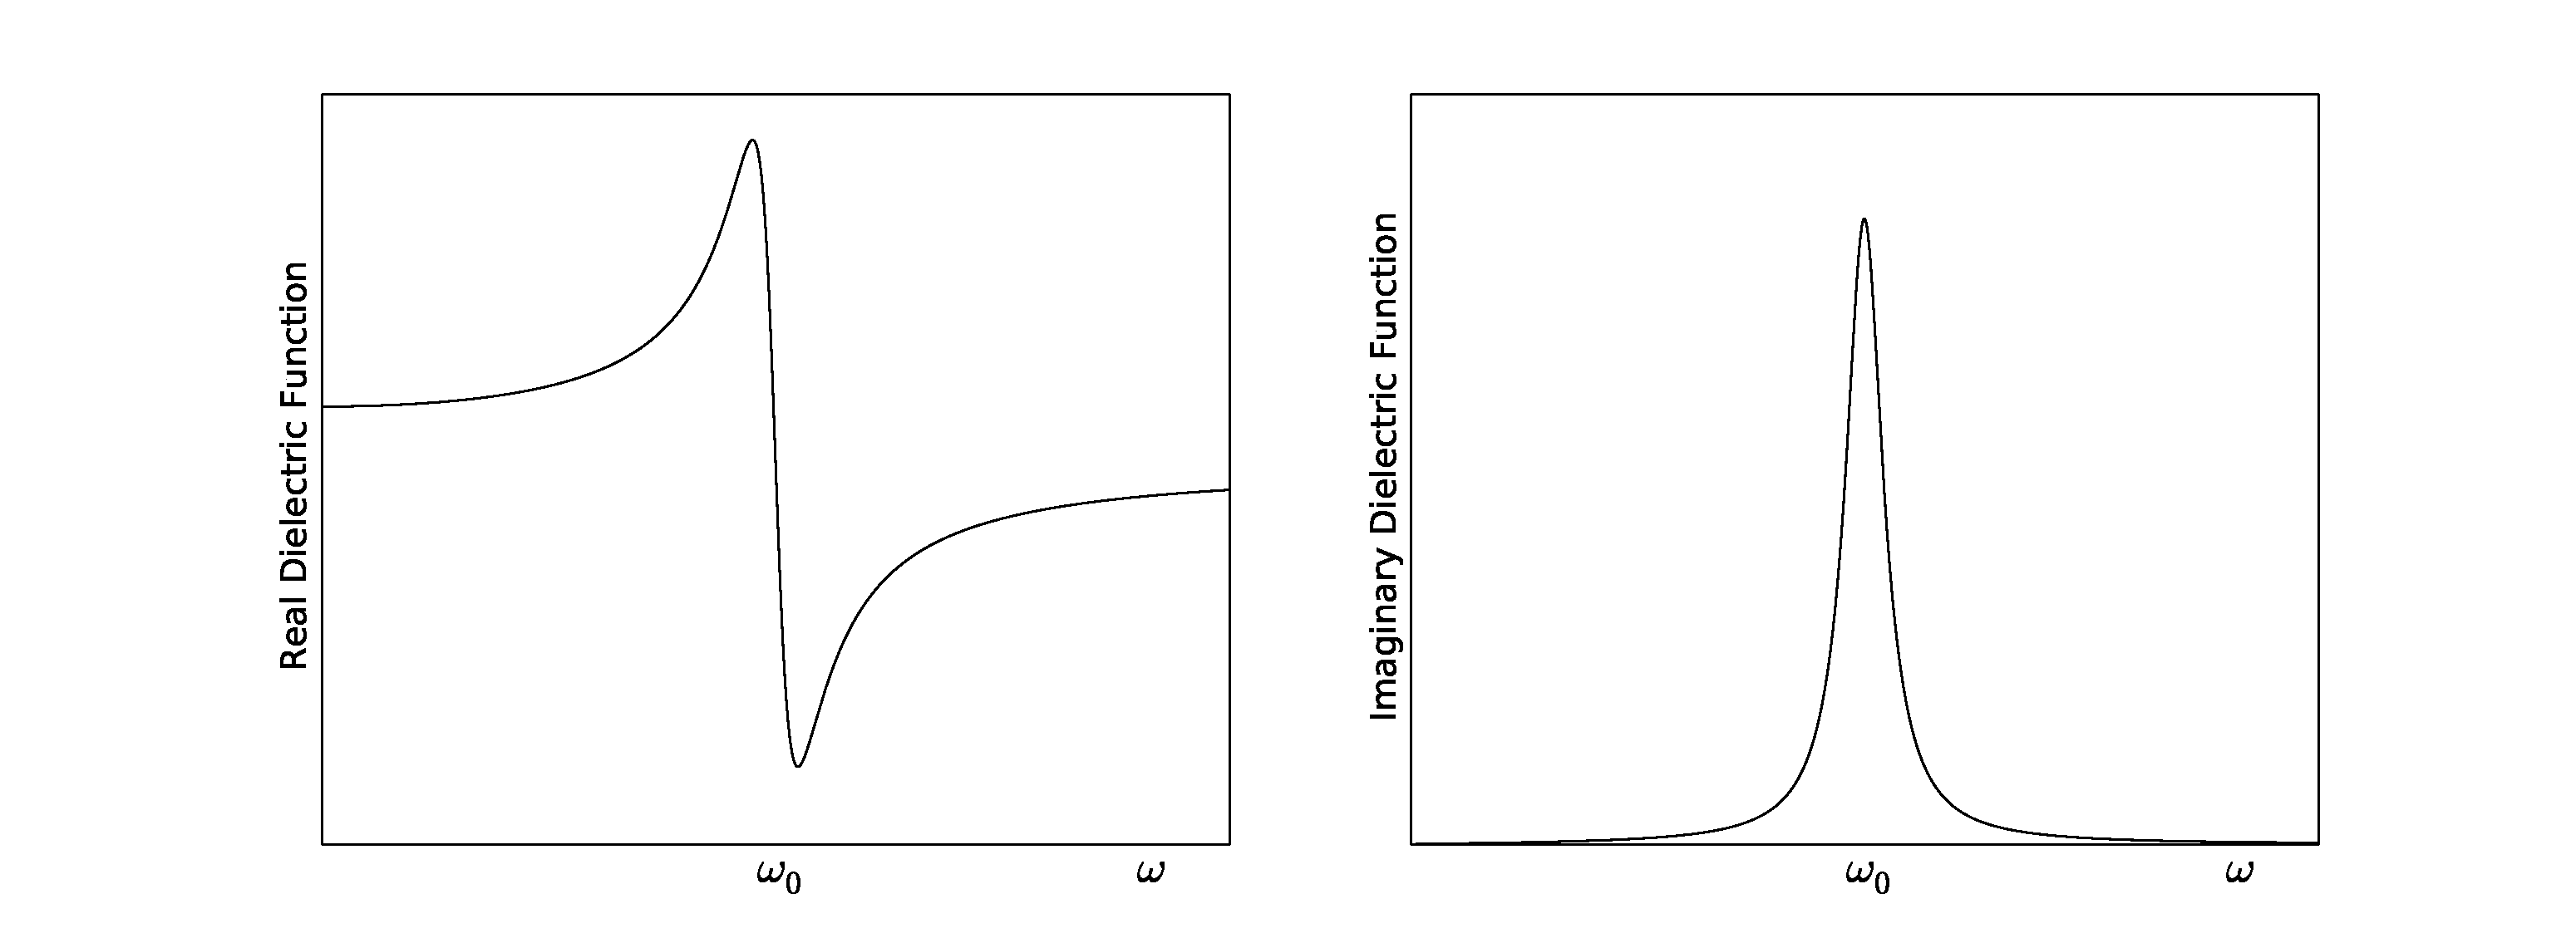
\includegraphics[width=1.0\textwidth]{../Figures/dielectricResonance.pdf}
   \caption{
      The dielectric function of a ionic crystal approximated by
      a driven harmonic oscillator with damping. The left and right figures show the behavior
      of the real and imaginary dielectric function close to
      the resonance frequency $\omega_0$.
   }
   \label{fig:dielectricResonance}
\end{figure}
%
The real part $\varepsilon\!_{_{\Re\! e}} \!\! (\omega)$ is almost constant away from the resonance
frequency, but its value is higher at lower frequencies due to the loss of the contribution from the
ionic polarization. The imaginary part $\varepsilon\!_{_{\Im\! m}} \!\! (\omega)$ is however zero 
everywhere except at the vicinity of the resonant frequency, where it shows a peak with a width
given by the damping coefficient $\eta$. 
\\
\\
To understand the meaning of $\varepsilon\!_{_{\Im\! m}} \!\! (\omega)$ and that the width
if its resonance peak is connected to the damping coefficient $\eta$, one can consider the
energy dissipation in the system. The instantaneous electrical power dissipated per unit 
volume is given by
\begin{align}
   P(t) = j(t)E(t) = j(t)Ee^{- i \omega t}
\end{align}
where j(t) is the curent density. In an insulator, there are no free currents, only polarization currents
\begin{align}
   j(t) = - \frac{\partial D}{\partial t} 
   = - \frac{\partial}{\partial t} \varepsilon \varepsilon_0 Ee^{- i \omega t}
   = i \omega \varepsilon \varepsilon_0 Ee^{- i \omega t}
\end{align}
The average dissipated power is found by averaging over one cycle $T = 2 \pi/\omega$
\begin{align}
   P = \frac{1}{T} \int_0^T E(t)j(t).
\end{align}
If $\varepsilon$ is purely imaginary, $j(t)$ is out of phase with $E(t)$ and their product will always
give a nonzero negative value,$-\varepsilon_0 \varepsilon\!_{_{\Im\! m}} \!\! (\omega) E^2$. On the other
hand, if $\varepsilon$ is purely real, the phase shift will be $\pi/2$ and the integral will give $P = 0$.
$\varepsilon\!_{_{\Im\! m}} \!\! (\omega)$ is therefore a measure of the energy dissipation of the
electric field due to the solid, and is obviously highest at the resonance.
\\
\\
The discussion explains some of the optical behaviour of the material. This is however not the
entire picture. E.g. the frequency dependence in the visible and UV region is not explained here.
These effects are due to the valence electrons, which would need a quantum mechanical description
of the electronic structure of the solid. From the band structure of solids, a qualitative
undestanding is obtainable. Figure \ref{fig:transitionResonance} shows regions of high photon absorbtion
due to the excitation of electrons, and how it is given by the imaginary dielectric function 
$\varepsilon\!_{_{\Im\! m}} \!\! (\omega) ? \varepsilon_i(\omega)$. Note that the photons do not have
enough energy to change the electrons wave vector
%
\begin{figure}[h!]
  \centering
   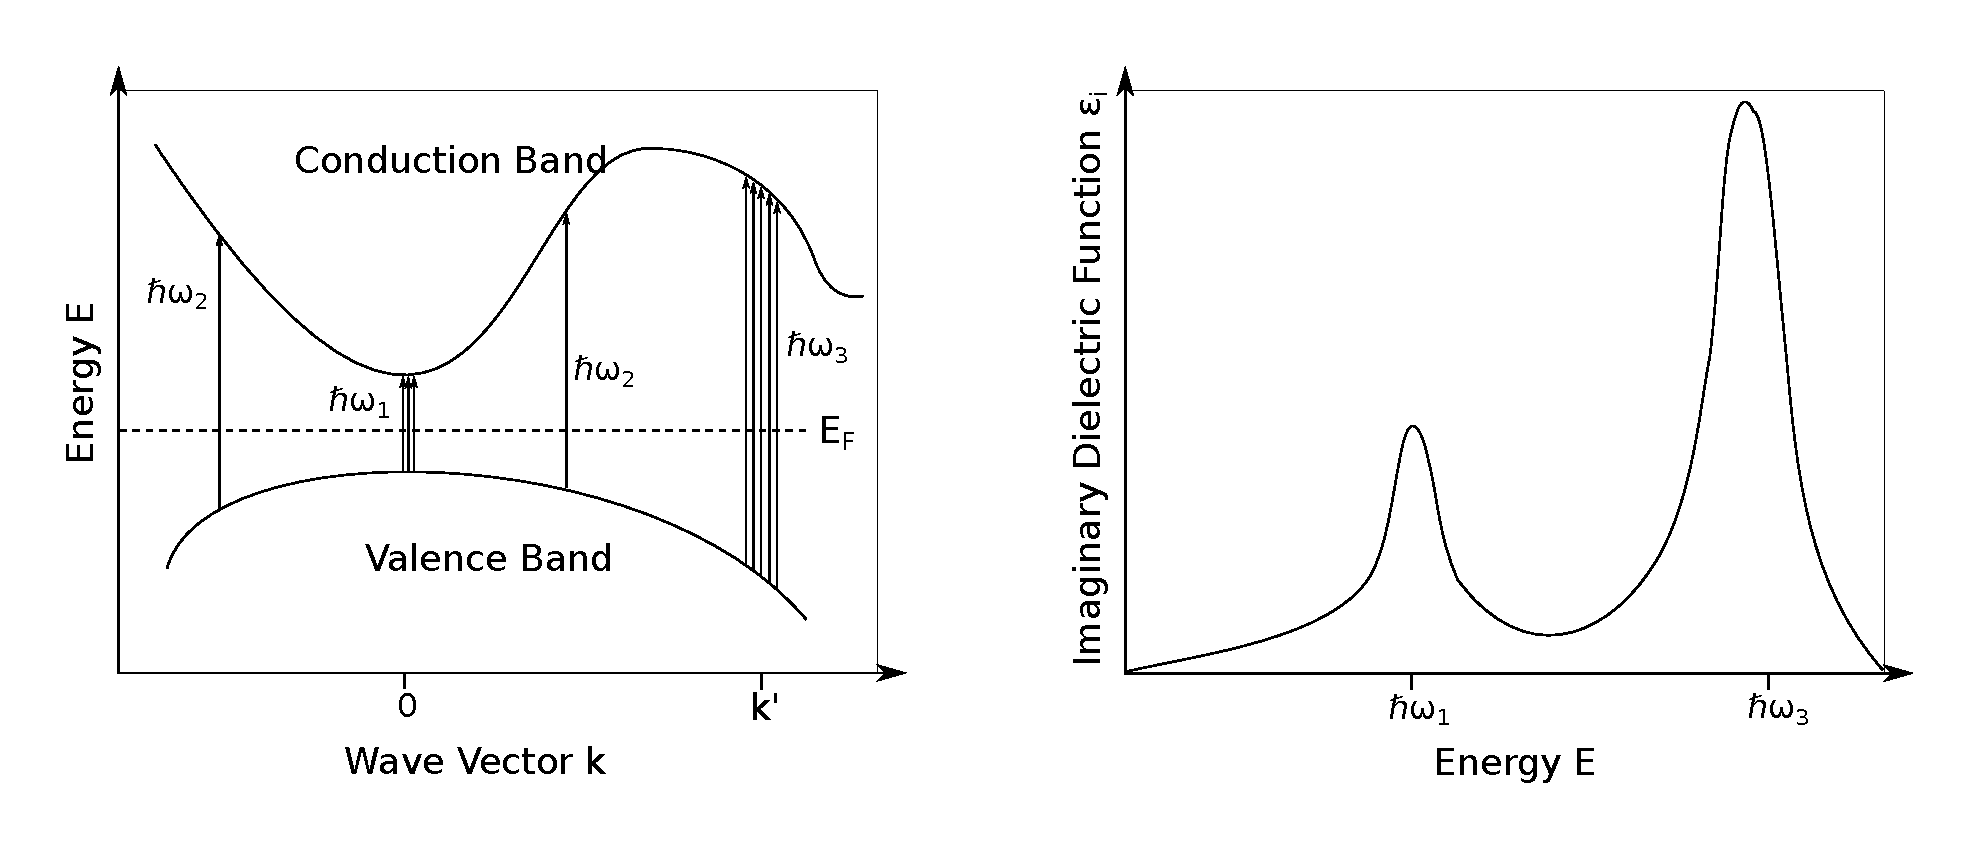
\includegraphics[width=1.0\textwidth]{../Figures/bandstructureVSdielectric.pdf}
   \caption{
      The left figure shows the photon-induced transitions between occupied and unoccupied states in the band 
      structure of a solid. $E_F$ is the fermi energy. 
      In the regions where the valence band and conduction bads are parallel,
      a certain photon energy can excite several states. Here, the parallel regions are located at
      $\boldsymbol k = 0$ and $\boldsymbol k = \boldsymbol k'$ and result in higher transitions density.
      These transitions correspond to absorbtion of the electromagnetic wave given by the imaginary part of
      the dielectric function $\varepsilon_i$. The resulting resonances in $\varepsilon_i$ due to 
      the absorbtion of the $\hbar \omega_1$ and $\hbar \omega_2$ transitions are depicted in the right
      figure.
   }
   \label{fig:transitionResonance}
\end{figure}
%






\begin{thebibliography}{9}

      \bibitem{Hofmann}
         Hofmann P.
         Solid State Physics, An Introduction.
         Wiley-VCH 2008; p.71-74,76-81

\end{thebibliography}




\subsection{Complex permittivity and index of refraction \cite[p.~169-170]{Jensen1985}}
%Jensen B: The Quantum Extension of the Drude-Zener Theory in Polar Semiconductors; p.169-188
The complex dielectric constant or relative permittivity 
$\widehat\varepsilon_r = \varepsilon_r + i \tilde\varepsilon_r$ of a material, is a measure of 
the material's response subject to an electromagnetic field. Here $\varepsilon_r$ and $\tilde\varepsilon_r$ 
denotes the real and imaginary components, respectively.
The relative permittivity is related to
the square of the refractive index, 
\begin{align}
   N^2 = \widehat\varepsilon_r
   \label{compEps}
\end{align}
which determines the optical properties of a given material.
It is like the dielectric constant complex
\begin{align}
   N = n + i k.
\end{align}
The real and imaginary refractive indicies are denotes by $n$ and $k$, respectively
The choice of sign convention, i.e. using $n+ik$ rather than $n-ik$, is determiend by 
the choice of the sign in the in the plane wave solution,
$\exp i(\boldsymbol q \cdot \boldsymbol r - \omega t )$, of
Maxwell's equations.
%The refractive index is also related to the conductivity $\sigma$
%\begin{align}
   %2nk = \frac{4\pi \sigma}{\omega}.
%\end{align}
%
From Eq.\eqref{compEps}
\begin{align}
   \widehat{\varepsilon}_r &= N^2 \\
   \varepsilon_r + i\tilde{\varepsilon}_r &= (n + ik)^2 \\
   \varepsilon_r + i\tilde{\varepsilon}_r &= n^2 - k^2 + i2nk,
\end{align}
and with some simple comparison, the components of the permittivity can be expressed as
\begin{align}
   \varepsilon_r &= n^2 - k^2     &\tilde{\varepsilon}_r  &= 2nk.
\end{align}
Taking the absolute value or modulus,
\begin{align}
   &\big|\widehat\varepsilon_r\big|   = \sqrt{ \varepsilon_r^2 + \tilde{\varepsilon}_r^2} \\
   &\big|\widehat\varepsilon_r\big|   = \sqrt{ (n^2 - k^2)^2 + (2nk)^2} \\
   &\big|\widehat\varepsilon_r\big|^2 = n^4 + 2n^2k^2 + k^4 \\
   &\big|\widehat\varepsilon_r\big|^2 = (n^2 + k^2)^2 \\
   &\big|\widehat\varepsilon_r\big|   = n^2 + k^2,
\end{align}
and putting it all together, gives the real and imaginary parts of $N$ expressed through the 
relative permettivity
\begin{align}
   n      &= \Bigg( \frac{\big|\widehat\varepsilon_r\big| + \varepsilon_r}{2}           \Bigg)^{\frac{1}{2}} 
           %= \Bigg( \frac{\big|\widehat\varepsilon  \big| + \varepsilon}{2\varepsilon_0}\Bigg)^{\frac{1}{2}}
  &k &=      \Bigg( \frac{\big|\widehat\varepsilon_r\big| - \varepsilon_r}{2}           \Bigg)^{\frac{1}{2}} 
           %= \Bigg( \frac{\big|\widehat\varepsilon  \big| - \varepsilon}{2\varepsilon_0}\Bigg)^{\frac{1}{2}}
\end{align}

Considering a plane wave with a complex wave vector $\widehat q = q + i \tilde q$ moving in the material
\cite[p.~402]{Griffiths}
\begin{align}
  e^{i(\widehat q z - \omega t )} 
  = e^{-\tilde q z} e^{i q z - \omega t )} ,
\end{align}
one sees that the wave is attenuated. 
The quantity $\alpha \equiv 2 \tilde q$ is called the absorption coeffiecient
and is proportional to the optical conductivity $\sigma$, to $\tilde\varepsilon$, and to $k$:
\begin{align}
   n\alpha = &\frac{4 \pi \sigma}{c} = \frac{\omega}{c} \tilde\varepsilon\\
                     &\Downarrow \\
   \frac{\alpha}{2} = &\frac{\omega}{c}k = \frac{1}{\delta}
\end{align}
$k$ is usually called the extinction coefficient and is essentially the ratio of the
free-space wave frequency $\omega$ to the skin depth $\delta$.\\


%Experimentally, $n$ and $k$ are found from measurements of the reflectivity R of a bulk, opaque sample
%and the transmittance T of a slab, which are given in terms of $n$ and $k$ as
$n$ and $k$ can be found experimentally by measuring the reflectivity R of a bulk, opaque sample,
in addition to the transmittance T of a slab, which are given in terms of $n$ and $k$ as
\begin{align}
   R &= \frac{(n-1)^2 + k^2}{(n+1)^2 + k^2} \\
   T &= \frac{ (1-R)^2 e^{-2\omega k d / c} }{ 1-R^2 e^{-4\omega k d / c} },
\end{align}
where $d$ is the sample thickness. The slab multiple-reflection effects are averaged,
so that interface fringes are not resolved.
%
\begin{thebibliography}{9}

      %Main article for dielectric function vs refractive index:
      \bibitem{Jensen1985}
       Jensen B.
       The quantum extension of the Drude-Zener theory in polar Semiconductors.
       Handbook of optical constants of Solids, Five-Volume 1997 (1985??)(9)<-it's chapter 9;169-170

      \bibitem{cambdridgePermittivityPage}.
         Dissemination of IT for the promotion of Materials Science (2000)
         Variation of the dielectric constant in alternating fields.
         University of Cambridge 2004:
         http://www.doitpoms.ac.uk/tlplib/dielectrics/variation.php
         (24. August 2015).
         %My interp. of webpage source: 
         %Authors, title, stuff behind(like university?) year ,link (date of site access)
\end{thebibliography}
 %moved to notes
\section{Theory}
To understand the theoretical background behind GranFilm and scattering on diffuse surfaces, it is 
convenient to start with the simple case of scattering on a flat interface of two different half-infinite
media, see Figure !!FIGUREREF HERE!!.

The electric permittivity $\varepsilon$ and magnetic permeability $\mu$ of the media are given with subscript $1$ for the above media, and $2$ for the media below. 
Using Maxwell's equations
%
\begin{subequations}
\label{ME}
\begin{align}
   \nabla \cdot \boldsymbol{D} &= \rho \!_f           &\nabla\times\boldsymbol{E} &= - \frac{\partial \boldsymbol{B}}{\partial t} \label{ME1}\\
   \nabla \cdot \boldsymbol{B} &= 0                &\nabla \times \boldsymbol{H}&= \boldsymbol{J}\!_f + \frac{\partial \boldsymbol{D}}{\partial t}, \label{ME2}
\end{align}
\end{subequations}
%
where the electric fields, $\boldsymbol{E}$ and $\boldsymbol{D}$, and magnetic fields $\boldsymbol{B}$ and $\boldsymbol{H}$ are related through
\begin{align}
   &\boldsymbol{D} = \varepsilon \boldsymbol{E},         &\boldsymbol{H} = \frac{1}{\mu} \boldsymbol{B}
\end{align}
(assuming linear media), the fields above $\boldsymbol{E}^+(\boldsymbol{r})$ and below $\boldsymbol{E}^-(\boldsymbol{r})$ the interface can be calculated for a incident place wave 
(same goes for $\boldsymbol{B}$, $\boldsymbol{D}$ and $\boldsymbol{H}$).
So far, the boundary between the two half-infinite media has been considered to be a sharp, flat discontinuity in $\varepsilon(z)$ and $\mu (z)$. 
As soon as the surface roughness, thickness and/or impurities are taken into acount, the complexity of the problem increases.


\textbf{From ''GranFilm-Software-Article''}: \\
Information on the dieletric behavior of surfaes can often be obtained by measuring the Fresnel coefficients,
such as reflection, transmission and absorption. \\
?p.2?: for a layer with thickness negligible compared to wavelength, we introduce surface susceptibilities 
which interconnect the  fresnel coeff. and characterise the optical response of the surface. ?? DID I UNDERSTAND THIS CORRECTLY? ?? \\
Since all the Fresnel coeff. can be expressed in terms of these surface susceptibilities, the main task consist of calculating these coefficients for the appropriate geometry. \\
\textbf{Goal of GranFilm:} to calculate ?surface-susceptibility-/fresnel-coefficients? and the associated measurableFresnel quantities for various surface layer geometries. 
\begin{itemize}
\item GranFilm is free open-source software
\end{itemize}
\subsection{Mie resonances/ plasmon absorption modes}
\textbf{From ''GranFilm-Software-Article''}: \\
when small metallic particles, the resonances can be absorbed by visible light and strongly affect the fresnel 
coefficients depending on the particle morphology.
%
\subsection{Quasistatic Approximation}
%
\subsection{Electromagnetic excess fields }
%
\textbf{From ''GranFilm-Software-Article''}: \\
(Bedeaux and Vlieger) \\
Difference between the bulk extrapolated fields and the real fields. The BC at the dividing surface
(which drive all fresnel coeff.) are given in terms of the integrated excess fields perpendicular to
the surface. \\
Bedeaux and Vlieger $\rightarrow$ formalism of excess quantities (does not require exact knowledge of the near suface EM-field behaviour). \\
Excess fields are defined as the differene between the real fields and the bulk fields extrapolated to the surface. E.g. for the electric field $E(r)$ the excess quantity is defined as
\begin{align}
   E_{ex} (r) = E(r) - E^-(r) \theta(-z) - E^+(r)\theta(z),
\end{align}
where $\theta(z)$ is the Heaviside function and the superscript $\pm$ are used to indicate the region above (+) and below (-) the dividing interface at $z = 0$. 
The excess field is only significant close to the surface, since $E(r, \omega) \rightarrow \rightarrow E^{\pm}(r,\omega)$  for $z \rightarrow \pm \infty$. \\
\textit{QUESTION: \@ Is the $E^{\pm}$ field solved for a infinite homogeneous medium of type (+) and (-) respectively  OR the field in simple two media interface scattering?} \\
\textbf{From Leif Amund Lies Msc Thesis}: \\
Since the excess fields will only be significant close to the surface, they may be thought of as perturbations to the simple case of flat interface. 
\textit{OWN INTERPRETATION: \@ This meas that the bulk fields are the fields created from scattering in the interface between two half-infinite media.} \\
Instead of tediously using the quasi-static-"no source"-BC, the excess fields defined as for the electric field above are inserted into the full Maxwell equations to derive new non-sharp boundary conditions.
The result reads
%
\textbf{From Leif Amund Lies Msc Thesis AND GranFilm-Article}: \\
%
\begin{subequations}
   \label{exFieldBC} % Excess Field Boundary Conditions
\begin{align}
   \big[ \boldsymbol{E}^+_{\parallel} (\boldsymbol{r}) - \boldsymbol{E}^-_{\parallel} (\boldsymbol{r}) \big] \bigg\rvert _{z = 0} 
       &= i \omega \hat{z} \times \! \boldsymbol{M}^s_{\parallel}(\boldsymbol{r}_{\parallel}) \:-\: \nabla\!_{\parallel} P^s_{z}(\boldsymbol{r}_{\parallel}) 
       \label{exFieldBC1} \\ 
   \big[ D^+_{z} (\boldsymbol{r}) - D^-_{z} (\boldsymbol{r}) \big] \bigg\rvert _{z = 0} 
      &= - \nabla\!_{\parallel} \boldsymbol{P}^s_{\parallel}(\boldsymbol{r}_{\parallel}) 
      \label{exFieldBC2} \\ 
   \big[ \boldsymbol{H}^+_{\parallel} (\boldsymbol{r}) - \boldsymbol{H}^-_{\parallel} (\boldsymbol{r}) \big] \bigg\rvert _{z = 0} 
      &= i \omega \hat{z} \times \! \boldsymbol{P}^s_{\parallel}(\boldsymbol{r}_{\parallel}) \:-\: \nabla\!_{\parallel} M^s_{z}(\boldsymbol{r}_{\parallel})  
      \label{exFieldBC3} \\ 
   \big[ B^+_{z} (\boldsymbol{r}) - B^-_{z} (\boldsymbol{r}) \big] \bigg\rvert _{z = 0} 
      &= - \nabla\!_{\parallel} \boldsymbol{M}^s_{\parallel}(\boldsymbol{r}_{\parallel}), 
      \label{exFieldBC4}  
\end{align}
\end{subequations}
%
which is derived in Vlieger and Bedaux's \textit{Optical Properties of Surfaces} (p.21). Here the quantities with superscript $s$ are the so-called excess polarization and magnetization densities
\begin{subequations}
\label{surfQuant} %Surface Quantities
\begin{align}
   \boldsymbol{P}^s(\boldsymbol{r}\!_{\parallel}) &= \big( \boldsymbol{D}^s_{\parallel}(\boldsymbol{r}\!_{\parallel}), \:\: - \varepsilon_0 E^s_{z}(\boldsymbol{r}\!_{\parallel}) \big) \label{surfQuant1}\\
   \boldsymbol{M}^s(\boldsymbol{r}\!_{\parallel}) &= \big( \boldsymbol{B}^s_{\parallel}(\boldsymbol{r}\!_{\parallel}), \:\: - \mu_0 H^s_{z}(\boldsymbol{r}\!_{\parallel}) \big) , \label{surfQuant2}
\end{align}
\end{subequations}
and the quantities on the right hand side are the excess fields integrated along the z-axis,
\begin{subequations}
\label{intExQuant} % integrated excess quantities
\begin{align}
   \boldsymbol{D}^s_{\parallel}(\boldsymbol{r}) &= \!\!\!\!\!\!\!\!\! \int\limits ^{\:\:\:\:\:\:\:\:\:\:+\infty}_{\!\!\!\!\!\!\!\!\!\!\!\!\!\!\!-\infty} \!\!\!\!\!\!\!\!\! d\!z\: \boldsymbol{D}\!_{ex,\parallel}(\boldsymbol{r}),
   &E^s_{z}(\boldsymbol{r}) = \!\!\!\!\!\!\!\!\! \int\limits ^{\:\:\:\:\:\:\:\:\:\:+\infty}_{\!\!\!\!\!\!\!\!\!\!\!\!\!\!\!-\infty} \!\!\!\!\!\!\!\!\! d\!z\: E\!_{ex,z}(\boldsymbol{r}) \label{intExQuant1}\\
   \boldsymbol{B}^s_{\parallel}(\boldsymbol{r}) &= \!\!\!\!\!\!\!\!\! \int\limits ^{\:\:\:\:\:\:\:\:\:\:+\infty}_{\!\!\!\!\!\!\!\!\!\!\!\!\!\!\!-\infty} \!\!\!\!\!\!\!\!\! d\!z\: \boldsymbol{B}\!_{ex,\parallel}(\boldsymbol{r}),
   &H^s_{z}(\boldsymbol{r}) = \!\!\!\!\!\!\!\!\! \int\limits ^{\:\:\:\:\:\:\:\:\:\:+\infty}_{\!\!\!\!\!\!\!\!\!\!\!\!\!\!\!-\infty} \!\!\!\!\!\!\!\!\! d\!z\: H\!_{ex,z}(\boldsymbol{r}). \label{intExQuant2}
\end{align}
\end{subequations}
\textit{OWN INTERPRETATION: These integrated excess quantities are equivalent of representing the the excess fields in a single Dirac term $\delta (z)$ located at the surface ($z = 0$), e.g. such that the electric field can be 
written as}
%
\begin{align}
   E(r) =  E^-(r) \theta(-z) + E^s(r)\delta (z) +  E^+(r)\theta(z).
\end{align}
%
\textit{OWN INTERPRETATION: Demanding that this fullfuls Maxwell's Equations, one obtains the Equations in \eqref{exFieldBC} }.
\textit{OWN INTERPRETATION: The simplest way to link the Surface polarization and magnetization density to the extrapolated bulk fields(?Sigma indexed fields?)involves a
symmetric constitutive tensor $\xi^s_e(\omega)$ (ref B,V-OPoS).}
\begin{align}
   \boldsymbol{P}^s(\boldsymbol{r}\!_{\parallel}) = \xi ^s_e \: \big[ \boldsymbol{E}_{\parallel, \Sigma}(\boldsymbol{r}\!_{\parallel}), \:\: - D\!_{z, \Sigma}(\boldsymbol{r}\!_{\parallel}) \big]
\end{align}
\textit{OWN INTERPRETATION: The above relation is restricted to non-magnetic materials, i.e. that $\boldsymbol{M}^s(\boldsymbol{r}\!_{\parallel}) = 0$.   The $\Sigma$ index denotes the arithmetic mean of the upper and lower
bulk fields, e.g. $ \boldsymbol{E}_{\parallel, \Sigma} = \big\{ \boldsymbol{E}^+_{\parallel} \!( \boldsymbol{r}\!_{\parallel} ) +  \boldsymbol{E}^-_{\parallel} \! (\boldsymbol{r}\!_{\parallel}) \big\} \big/2 $.
If the interface are z = 0 is isotropic and symmetric, the interfacial tensor $\xi ^s_e$ is diagonal}:
\begin{align}
\xi ^s_e = 
\begin{bmatrix}
   \gamma   &   0       &  0      \\
   0        &   \gamma  &  0      \\
   0        &   0       &  \beta 
\end{bmatrix}
.
\end{align}
Here the coefficients $\gamma$ and $\beta$ are called the (first-order) surface susceptibilities (or here, constitutive coefficients). The constitutive coefficients of second order, $\delta$ and $\tau$ describe
a non-local dependence (??SPATIAL VARIATIONS IN THE EXCESS QUANTITIES??) \\
\textbf{Fresnel Coefficients} \\
...need to write some more here...
\begin{subequations}
   \label{fresCoeffS}
\begin{align}
   r_s(\omega) &= \frac{n\!_{_-} \cos \theta_i - n\!_{_+} \cos \theta_t + i(\omega/c) \gamma}{n\!_{_-} \cos \theta_i + n\!_{_+} \cos \theta_t - i(\omega/c) \gamma} \label{fresCoeffS1} \\
   t_s(\omega) &= \frac{2 n\!_{_-} \cos \theta_i}{n\!_{_-} \cos \theta_i + n\!_{_+} \cos \theta_t - i(\omega/c) \gamma} \label{fresCoeffS2}
\end{align}
\end{subequations}
%
\begin{subequations}
\label{fresCoeffP}
\begin{align}
   r_p(\omega) &= \frac{\kappa\!_{_-}(\omega) -i(\omega / c) \gamma \cos \theta_i \cos \theta_t + i(\omega/c)n\!_{_-} n\!_{_+} \varepsilon\!_{_-}\beta\sin^2 \theta_i }
   {\kappa\!_{_+}(\omega) -i(\omega / c) \gamma \cos \theta_i \cos \theta_t - i(\omega/c) n\!_{_-} n\!_{_+} \varepsilon\!_{_-} \beta \sin^2 \theta_i }, \label{fresCoeffS1}\\
   t_p(\omega) &= \frac{2n\!_{_-} \cos \theta_i \big[ 1 + (\omega/2c)^2 \varepsilon\!_{_-} \gamma \beta \sin ^2 \theta_i \big]}
   {\kappa\!_{_+}(\omega) -i(\omega / c) \gamma \cos \theta_i \cos \theta_t - i(\omega/c) n\!_{_-} n\!_{_+} \varepsilon\!_{_-} \beta \sin^2 \theta_i }, \label{fresCoeffS2}\\
   \kappa\!_{\pm} &= \big[ n\!_{_+} \cos \theta _i \pm n\!_{_-} \cos \theta_t  \big]\Bigg[ 1 - \frac{\omega^2}{4c^2} \varepsilon\!_{_-} \gamma \beta \sin ^2 \theta_i \Bigg]. \label{fresCoeffS3}
\end{align}
\end{subequations}
%
%\begin{subequations}
%\begin{align}
   %r_p(\omega) &= \frac{\kappa _-(\omega) -i(\omega / c) \gamma \cos \theta_i \cos \theta_t + i(\omega/c)n_-n_+\varepsilon_-\beta\sin^2 \theta_i }
               %{\kappa _+(\omega) -i(\omega / c) \gamma \cos \theta_i \cos \theta_t - i(\omega/c)n_-n_+\varepsilon_-\beta\sin^2 \theta_i } \\
   %t_p(\omega) &= \frac{2n_- \cos \theta_i \big[ 1 + (\omega/2c)^2 \varepsilon_- \gamma \beta \sin ^2 \theta_i \big]}
               %{\kappa _+(\omega) -i(\omega / c) \gamma \cos \theta_i \cos \theta_t - i(\omega/c)n_-n_+\varepsilon_-\beta\sin^2 \theta_i } \\
   %\kappa_{\pm} &= \big[ n_+ \cos \theta _i \pm n_- \cos \theta_t  \big]\Bigg[ 1 - \frac{\omega^2}{4c^2} \varepsilon_- \gamma \beta \sin ^2 \theta_i \Bigg]
%\end{align}
%\end{subequations}
From Eq. \eqref{fresCoeff1}-Eq.\eqref{fresCoeff3} we can observe that $p$-polarized excite the surface in both parallel and perpendicular direction, relative to the surface. 






\subsection{.}


\textbf{D'Alembert Operator $\square$}
\begin{align*}
  \square  &= \partial ^{\mu} \partial _{\mu}
   \\
           &= \frac{1}{c^2} \frac{\partial ^2}{\partial t^2} 
               - \frac{\partial ^2}{\partial x^2} 
               - \frac{\partial ^2}{\partial y^2} 
               - \frac{\partial ^2}{\partial z^2} 
   \\
           &= \frac{1}{c^2} \frac{\partial ^2}{\partial t^2} - \nabla ^2
\end{align*}

\textbf{Lorentz Gauge:} \\
For Lorentz invariance, convenient to choose the Lorenz gauge:
\begin{align*}
   \square \vec{A} = \Bigg[ \frac{1}{c^2} \frac{\partial ^2}{\partial t^2} - \nabla ^2 \Bigg] \vec{A} = \mu_0 \vec{J}
\end{align*}
\begin{align*}
   \square \phi = \Bigg[ \frac{1}{c^2} \frac{\partial ^2}{\partial t^2} - \nabla ^2 \Bigg] \phi = \frac{\rho}{\epsilon _0}
\end{align*}




\section{\textbf{The theory behind GranFilm}}
%To understand the theoretical background behind GranFilm and scattering on diffuse surfaces, it is 
%convenient to start with the simple case of scattering on a flat interface of two different half-infinite
%media, see Figure !!FIGUREREF HERE!!.
This section discusses the theoretical background behind GranFilm, a software used to calculate
the optical properties of granular thin films. The software implemented by Simonsen and Lazzari
is based on the theory developed by Bedeaux and Vlieger \cite{BedeauxVliegerBook} which introduces
so called excess fields to handle the complexity of the surface. Before we dive into the details
of this approach it might be beneficial to first consider scattering from flat surfaces.

\subsection{Theoretical Introduction; Flat Surface Scattering} \label{sectionFlatScattering}
Starting from basic electromagnetic theory, the simplest case 
of electromagnetic scattering is the transmission and reflection of light, hitting a flat,
smooth interface between two different half-infinite media. 
The electric permittivity $\varepsilon$ and magnetic permeability $\mu$ of the media are given 
with subscript $+$ for the upper media, and $-$ for the lower media, see Figure \ref{fig:flatScattering}. 
\begin{figure}[h!]
  \centering
   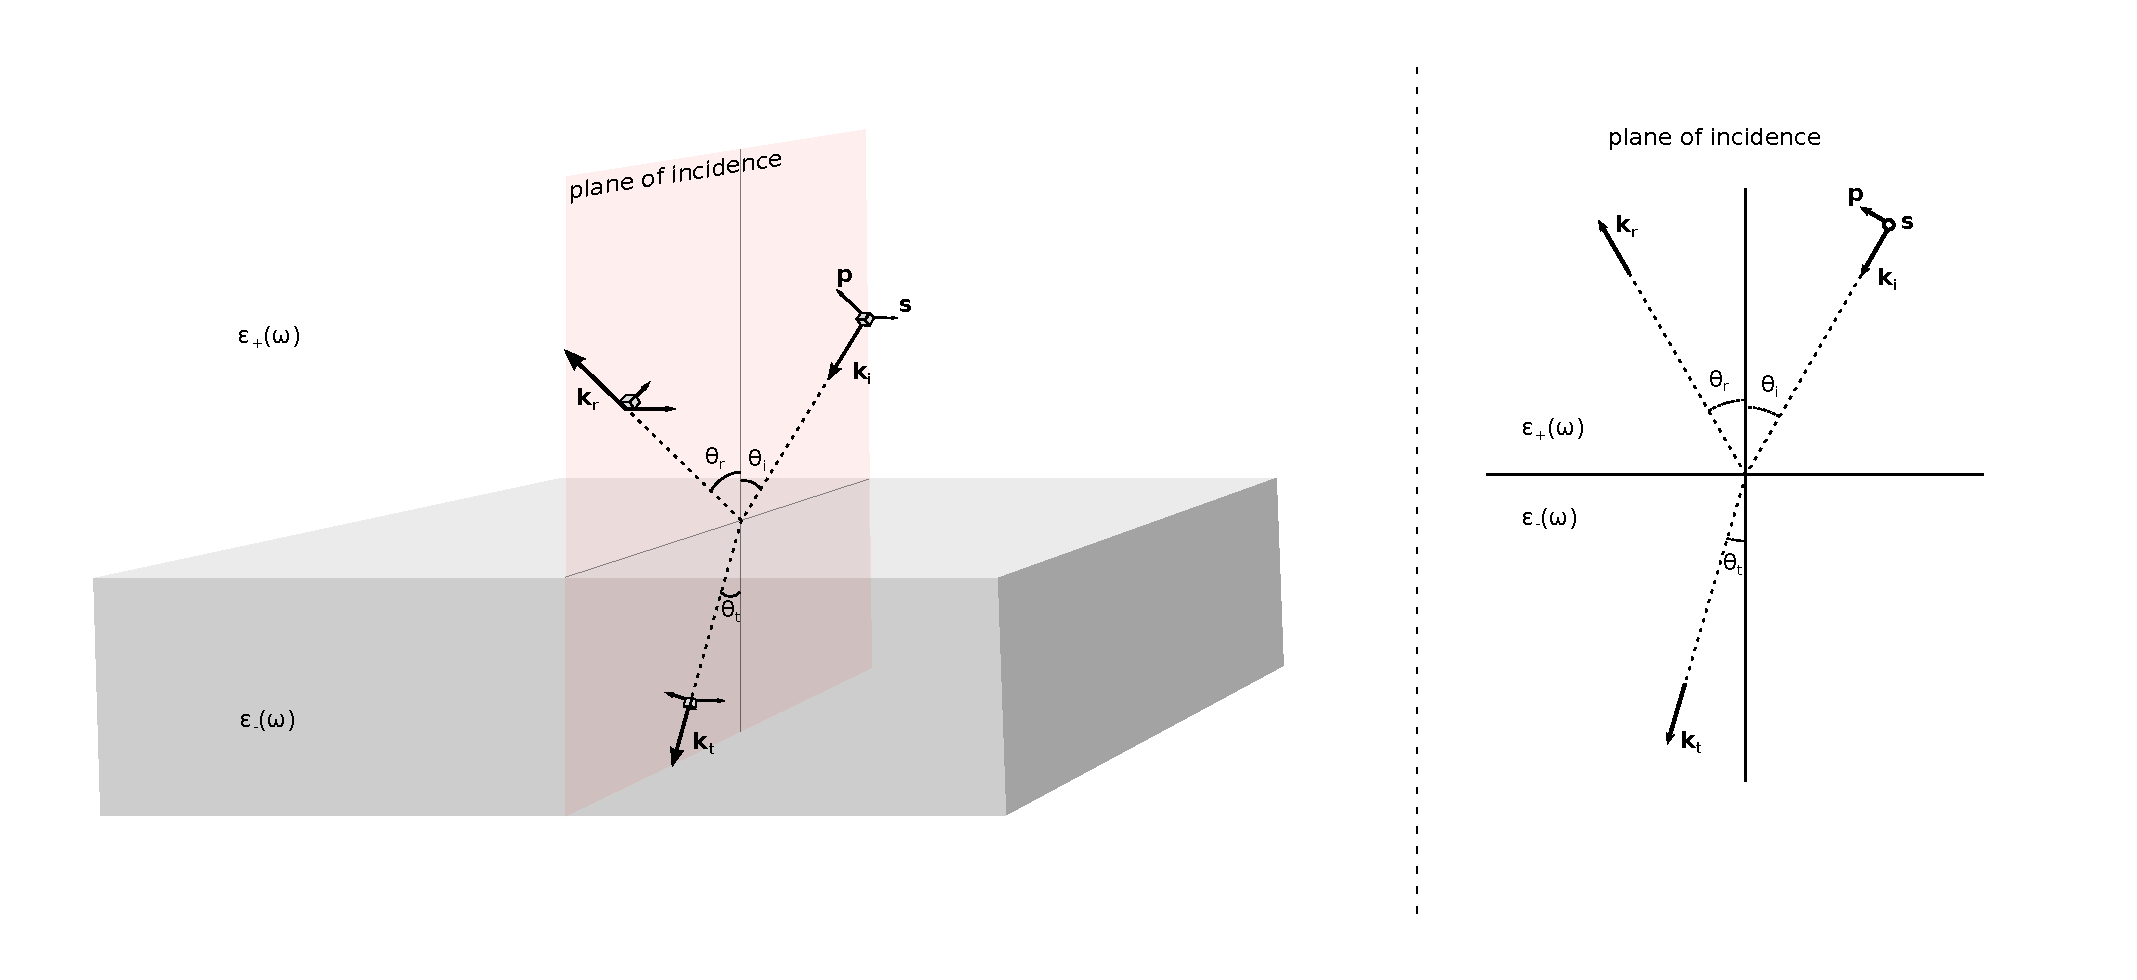
\includegraphics[width=1.0\textwidth]{Figures/flatSurfaceScattering.pdf}
   \caption{The reflection and transmission of an incident electromagnetic plane wave on a flat interface
      between two media. The dielectric functions for the upper and lower media are $\varepsilon_{+}(\omega)$
      and  $\varepsilon_{-}(\omega)$, respectively. The polarization direction $\boldsymbol{p}$ is the
      polarization parallel to or inside the place of incidence, while $\boldsymbol{s}$, which comes from the
      german word \textit{senkrecht} meaning perpendicular, is the perpendicular polarization.
      The figure is adopted from (\cite{Lazzari2002}, p.125).
   }
   \label{fig:flatScattering}
\end{figure}
Assuming that the incoming electromagnetic wave is a plane wave, the reflection and transmission
of the wave can be calculated from Maxwell's equations,
%
\begin{subequations}
\label{ME}
\begin{align}
   \nabla \cdot \boldsymbol{D} &= \rho \!_f           &\nabla\times\boldsymbol{E} &= - \frac{\partial \boldsymbol{B}}{\partial t} \label{ME1}\\
   \nabla \cdot \boldsymbol{B} &= 0                &\nabla \times \boldsymbol{H}&= \boldsymbol{J}\!_f + \frac{\partial \boldsymbol{D}}{\partial t}, \label{ME2}
\end{align}
\end{subequations}
%
which describe the general behavior of electromagnetic waves.
Here the electric field $\boldsymbol{E}$, the electric displacement $\boldsymbol{D}$,
the magnetic field $\boldsymbol{H}$ and the magnetic induction $\boldsymbol{B}$
are pairwise related through
\begin{align}
   \label{linearConstitutiveRelations}
   &\boldsymbol{D} = \varepsilon \boldsymbol{E},         &\boldsymbol{H} = \frac{1}{\mu} \boldsymbol{B},
\end{align}
assuming linear media \cite[p.~330]{Griffiths}. 
Further assuming that there
is no free charge or free current at the interface, Maxwell's equation provide the boundary conditions 
(\cite{Griffiths}, p.333)
%
\begin{subequations}
\label{BC}
\begin{align}
   D^+_{\perp} &= D^-_{\perp}      &\boldsymbol{E}^+_{\parallel} = \boldsymbol{E}^-_{\parallel} \label{BC1}\\
   B^+_{\perp} &= B^-_{\perp}      &\boldsymbol{H}^+_{\parallel} = \boldsymbol{H}^-_{\parallel}. \label{BC2}
\end{align}
\end{subequations}
%
($\perp$ and $\parallel$ denotes the perpendicular and parallel komponent with respect to the 
surface boundary. By enforcing these boundary conditions on the incident, reflected and transmitted 
waves, on the entire boundary, the reflection and transmission coefficients may be calculated. The 
coefficients are given by
\begin{align}
   R &\equiv \frac{I_r}{I_i}     &T &\equiv \frac{I_t}{I_i}, \label{refTransCoeffs1}\\
\end{align}
where $I_x, x \in [i,r,t]$ is the intensity or power per unit area stricking/leaving the interface
for the incident, reflected and transmitted light, respectively \cite[p.~386-391]{Griffiths}.
The calculation can be found in any standard optics textbook \cite{Smith} and gives
\begin{align}
   R &= r^2       &T &= \frac{n\!_{_-} \cos \theta_t}{n\!_{_+} \cos \theta _i}t^2. \label{refTransCoeffs2}\\
\end{align}
$n\!_{_+}$ and $n\!_{_-}$ are the indices of refraction for the media above (+) and belov (-) the interface,
while $\theta_i$ and $\theta_t$ gives the incident and transmitted lights direction with respect to the 
surface normal. 
The coefficients $r$ and $t$ are called the Frensel coefficients and their values depend on the
polarization of the incident light. For the flat interface the coefficients take the form
%
\begin{subequations}
\label{flatFresnelCoeff}
\begin{align}
   r_s &= \frac{n\!_{_+} \cos \theta_i - n\!_{_-} \cos \theta_t}
   {n\!_{_+} \cos \theta_i + n\!_{_-} \cos \theta_t}     
   &t_s &= \frac{2 n\!_{_+} \cos \theta_i}
   {n\!_{_+} \cos \theta_i + n\!_{_-} \cos \theta_t}, \label{flatFresnelCoeffs} \\
%
   r_p &= \frac{n\!_{_-} \cos \theta_i - n\!_{_+} \cos \theta_t}
   {n\!_{_+} \cos \theta_t + n\!_{_-} \cos \theta_i}     
   &t_p &= \frac{2 n\!_{_+} \cos \theta_i}
   {n\!_{_+} \cos \theta_t + n\!_{_-} \cos \theta_i}     \label{flatFresnelCoeffp}
\end{align}
\end{subequations}
%
so the reflection and transmission are different for the two polarization directions \cite[p.~121-123]{Smith}.
The two polarizations are illustrated in Figure \ref{fig:flatScattering}

\subsection{Scattering on rough surfaces: excess fields and surface susceptibilities}
When moving away from a flat surface towards a more complicated geometry of the boundary 
between the two media, the corresponding dielectric function also becomes complicated.
Situations like these might be encountered for rough surfaces or granular thin films, where the latter
means that a foreign material is distributed as small island on top of a substrate. 
With such a complicated boundary, the calculation of the Fresnel coefficients becomes more difficult.
\cite[p.~125]{Lazzari2002}.
\\
\\
However, Bedeaux and Vlieger \cite{BedeauxVliegerBook} %my old referance:(\cite{Lazzari2002}, (7-12)) 
developed an approach in which the exact knowledge
of the electromagnetic fields close to the surface is not required. Their formalism is based on the notion 
of excess quantities. 
The excess fields are defined as the differene between the real fields and the bulk fields extrapolated
to the surface, where the bulk field simply means the field given sufficiently far away from the
scattering surface. E.g. for the electric field $\boldsymbol E(r)$ the excess quantity is defined as
%
\begin{align}
   \label{excessField1}
   \boldsymbol{E}_{ex} (\boldsymbol{r}) \:=\: \boldsymbol{E}(\boldsymbol{r}) 
   \:-\: \boldsymbol{E}^-(\boldsymbol{r})\theta(-z) \:-\: \boldsymbol{E}^+(\boldsymbol{r})\theta(z),
\end{align}
%
where $\theta(z)$ is the Heaviside function and the superscript $\pm$ are used to indicate the region
above (+) and below (-) the dividing interface at $z = 0$. In addition, the optical frequency $\omega$
is implicitly included in the notation. Furthermore, the excess field is only significant close
to the surface, since $\boldsymbol{E}(\boldsymbol{r},\omega) \rightarrow 
\boldsymbol{E}^{\pm}(\boldsymbol{r},\omega)$ when $z \rightarrow \pm \infty$. \\
By integrating these excess fields along the z-axis, which is set normal to the surface,
%
\begin{subequations}
\label{intExQuant} % integrated excess quantities
\begin{align}
   \boldsymbol{D}^s_{\parallel}(\boldsymbol{r}) &= \!\!\!\!\!\!\!\!\! \int\limits ^{\:\:\:\:\:\:\:\:\:\:+\infty}_{\!\!\!\!\!\!\!\!\!\!\!\!\!\!\!-\infty} \!\!\!\!\!\!\!\!\! d\!z\: \boldsymbol{D}\!_{ex,\parallel}(\boldsymbol{r}),
   &E^s_{z}(\boldsymbol{r}) = \!\!\!\!\!\!\!\!\! \int\limits ^{\:\:\:\:\:\:\:\:\:\:+\infty}_{\!\!\!\!\!\!\!\!\!\!\!\!\!\!\!-\infty} \!\!\!\!\!\!\!\!\! d\!z\: E\!_{ex,z}(\boldsymbol{r}) \label{intExQuant1}\\
   \boldsymbol{B}^s_{\parallel}(\boldsymbol{r}) &= \!\!\!\!\!\!\!\!\! \int\limits ^{\:\:\:\:\:\:\:\:\:\:+\infty}_{\!\!\!\!\!\!\!\!\!\!\!\!\!\!\!-\infty} \!\!\!\!\!\!\!\!\! d\!z\: \boldsymbol{B}\!_{ex,\parallel}(\boldsymbol{r}),
   &H^s_{z}(\boldsymbol{r}) = \!\!\!\!\!\!\!\!\! \int\limits ^{\:\:\:\:\:\:\:\:\:\:+\infty}_{\!\!\!\!\!\!\!\!\!\!\!\!\!\!\!-\infty} \!\!\!\!\!\!\!\!\! d\!z\: H\!_{ex,z}(\boldsymbol{r}), \label{intExQuant2}
\end{align}
\end{subequations}
%
\begin{figure}[h!]
  \centering
   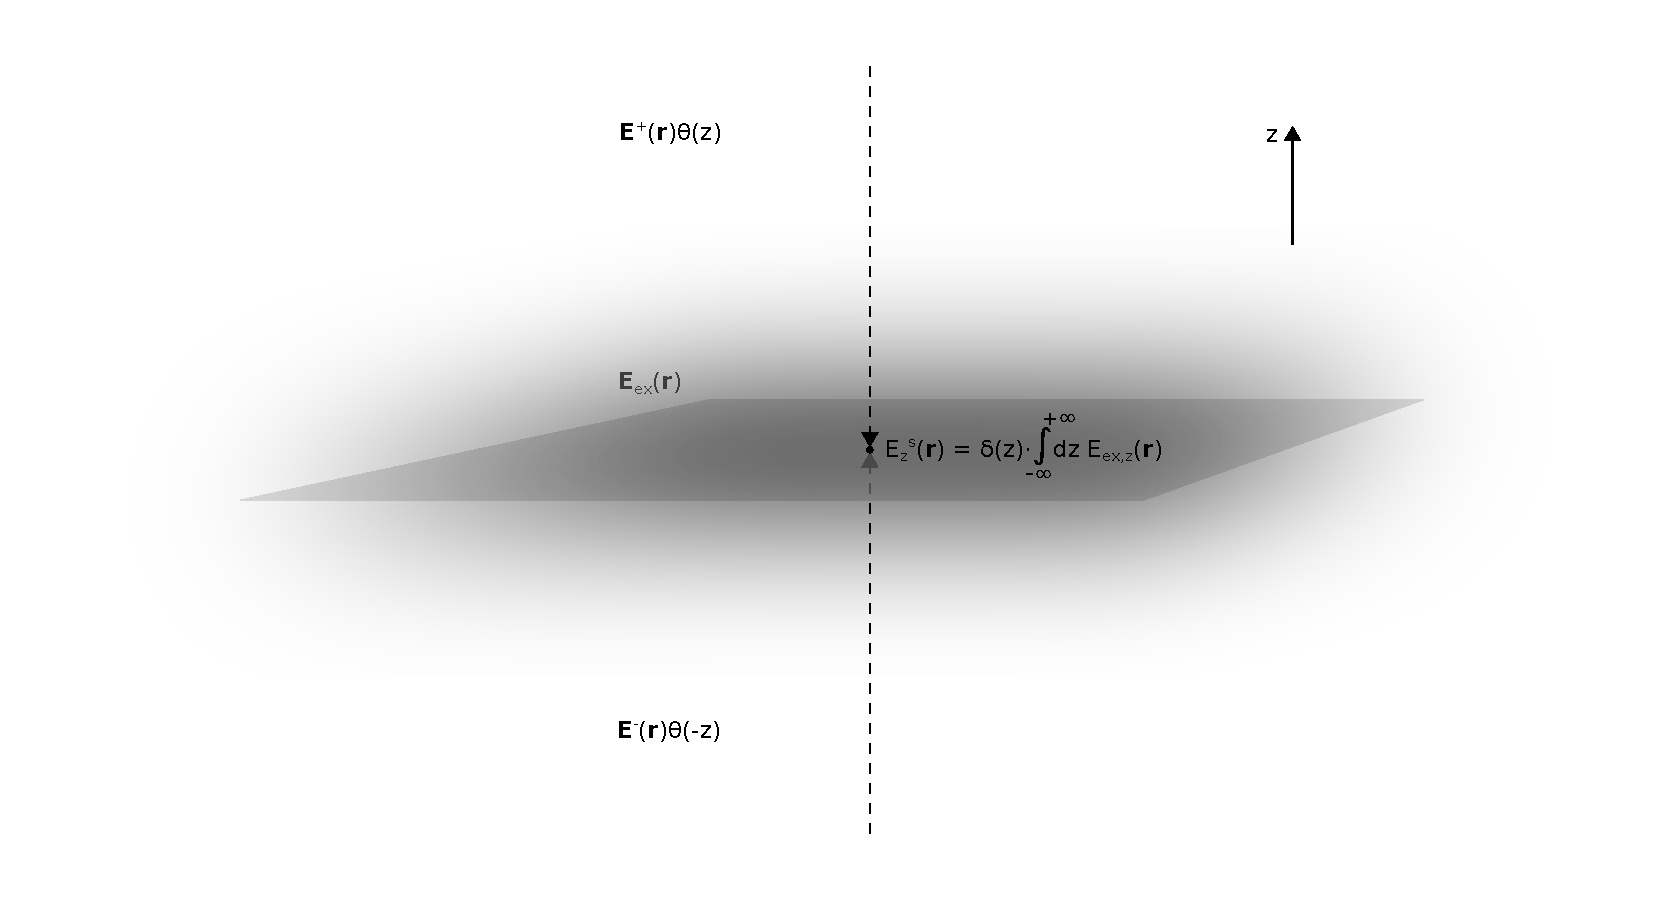
\includegraphics[width=1.0\textwidth]{Figures/excessFields.pdf}
   \caption{The excess fields are integrated over all values of z over the entire surface. Here this 
      is vizualized for the eletric excess field, vizualized by the fog surrounding the surface, as
      the excess field, is only significant close to the surface. Note however that the excess field
      is complicated and not correctly represented by the fog.  (\cite{Lazzari2002}, p.126).
   }
   \label{fig:excessFields}
\end{figure}
%
and gathering them in a singular Dircac term, $\delta(z)$, located at the surface (z=0)
(see Figure \ref{fig:excessFields},
the fields may be rewritten on the form (here shown for just the electric field)
%
\begin{align}
   \label{excessField2}
   \boldsymbol{E}(\boldsymbol{r}) \:=\: \boldsymbol{E}^-(\boldsymbol{r})\theta(-z) 
                                       \:+\: \boldsymbol{E}^s(\boldsymbol{r})\delta(z) 
                                       \:+\: \boldsymbol{E}^+(\boldsymbol{r})\theta(z).
\end{align}
%
Demanding that the fields given by Eq. \eqref{excessField2} fulfill the Maxwell equations 
one ends up with the following boundary conditions %(\cite{Lazzari2002}, (7-9))
%
\begin{subequations}
   \label{exFieldBC} % Excess Field Boundary Conditions
\begin{align}
   \big[ \boldsymbol{E}^+_{\parallel} (\boldsymbol{r}) - \boldsymbol{E}^-_{\parallel} (\boldsymbol{r}) \big] \bigg\rvert _{z = 0} 
       &= i \omega \hat{z} \times \! \boldsymbol{M}^s_{\parallel}(\boldsymbol{r}_{\parallel}) \:-\: \nabla\!_{\parallel} P^s_{z}(\boldsymbol{r}_{\parallel}) 
       \label{exFieldBC1} \\ 
   \big[ D^+_{z} (\boldsymbol{r}) - D^-_{z} (\boldsymbol{r}) \big] \bigg\rvert _{z = 0} 
      &= - \nabla\!_{\parallel} \boldsymbol{P}^s_{\parallel}(\boldsymbol{r}_{\parallel}) 
      \label{exFieldBC2} \\ 
   \big[ \boldsymbol{H}^+_{\parallel} (\boldsymbol{r}) - \boldsymbol{H}^-_{\parallel} (\boldsymbol{r}) \big] \bigg\rvert _{z = 0} 
      &= i \omega \hat{z} \times \! \boldsymbol{P}^s_{\parallel}(\boldsymbol{r}_{\parallel}) \:-\: \nabla\!_{\parallel} M^s_{z}(\boldsymbol{r}_{\parallel})  
      \label{exFieldBC3} \\ 
   \big[ B^+_{z} (\boldsymbol{r}) - B^-_{z} (\boldsymbol{r}) \big] \bigg\rvert _{z = 0} 
      &= - \nabla\!_{\parallel} \boldsymbol{M}^s_{\parallel}(\boldsymbol{r}_{\parallel}), 
      \label{exFieldBC4}  
\end{align}
\end{subequations}
%
which is derived by Vlieger and Bedaux \cite[p.21]{BedeauxVliegerBook}. 
Here $\nabla_{\parallel}$ is the nabla operator parallel to the surface, while $z$ denotes 
the vector component in the direction normal to the surface at $z = 0$.
In addition, the quantities with superscript $s$ are the so-called excess polarization 
and magnetization densities
\begin{subequations}
\label{surfQuant} %Surface Quantities
\begin{align}
   \boldsymbol{P}^s(\boldsymbol{r}\!_{\parallel}) &= \big( \boldsymbol{D}^s_{\parallel}(\boldsymbol{r}\!_{\parallel}), \:\: - \varepsilon_0 E^s_{z}(\boldsymbol{r}\!_{\parallel}) \big) \label{surfQuant1}\\
   \boldsymbol{M}^s(\boldsymbol{r}\!_{\parallel}) &= \big( \boldsymbol{B}^s_{\parallel}(\boldsymbol{r}\!_{\parallel}), \:\: - \mu_0 H^s_{z}(\boldsymbol{r}\!_{\parallel}) \big) , \label{surfQuant2}
\end{align}
\end{subequations}
Here, in Eq.\eqref{surfQuant}, the quantities on the right hand side
are the integrated excess fields.
%
%PROBLEMS WITH THE NEED FOR CONSTITUTIVE RELATIONS:
%\textit{?? IS THE FOLLOWING CORRECT??} 
%Now, as mentioned above, the excess quantities describe the 
%discontinuitiy in the bulk fields, through the interfacial polarisation and magnetisation desnity,
%$\boldsymbol{P}^s(\boldsymbol{r}_{parallel})$ $\boldsymbol{M}^s(\boldsymbol{r}_{parallel})$. This
%gives the field relations above and below the interface. To explain 
%
%OWN INTERPRETATION: The simplest way to link the surface polarization and magnetization density to the extrapolated bulk fields(?Sigma indexed fields?)involves a
Even though Maxwell's equations have been included, demanding that the fields follow the boundary 
conditions of Eqs.\eqref{exFieldBC}, they do not uniquely determine the physical situation. 
Maxwell's equations in matter, Eq.\eqref{ME} given in Section \ref{sectionFlatScattering}, includes
$\boldsymbol{E}$ and $\boldsymbol{D}$, together with $\boldsymbol{B}$ and $\boldsymbol{H}$, 
but does not state how they depend on eachother. In other words, Eq.\eqref{ME} does not contain
more information than Maxwell's equations given in free space. So, to fully explain how 
the fields interact with material and the interface, constitutive relations characteristic 
to the surface must be given (like the relations in Eq.\eqref{linearConstitutiveRelations} 
given for the flat interface example) \cite[p. 330]{Griffiths}.
The constitutive relations link the interfacial polarisation and 
magnetization density $\big(\boldsymbol{P}^s(\boldsymbol{r}_{\parallel})$ and 
$\boldsymbol{M}^s(\boldsymbol{r}_{\parallel}) \big)$ and the bulk fields extrapolated to the surface.
%To link the interfacial polarisation and 
%magnetization density, $\boldsymbol{P}^s(\boldsymbol{r}_{parallel})$ and 
%$\boldsymbol{M}^s(\boldsymbol{r}_{parallel})$, and the bulk fields extrapolated to the surface,
%additional relations, which are characteristic to the interface, must be given.
%
If the pertubed surface layer thickness $d$ is negligible compared to the optical wavelength $\lambda$,
the excess fields are only significant or non-negligible close to the surface, which followed
from the notation for the excess fields assumed earlier in Eq. \eqref{excessField1}.
Because of this, the constitutive relations are local and the extrapolated bulk fields may be written on the 
form 
$\boldsymbol{E}_{\parallel, \Sigma} = \big\{ \boldsymbol{E}^+_{\parallel} \!( \boldsymbol{r}\!_{\parallel} ) 
+  \boldsymbol{E}^-_{\parallel} \! (\boldsymbol{r}\!_{\parallel}) \big\} \big/2 $.
For simplisity we restrict our discussion to non-magnetic materials,
i.e. that $\boldsymbol{M}^s(\boldsymbol{r}_{\parallel}) = 0$. The simplest constitutive relation
can be written on the form
\begin{align}
   \boldsymbol{P}^s(\boldsymbol{r}\!_{\parallel}) = \xi ^s_e \: \big[ \boldsymbol{E}_{\parallel, \Sigma}(\boldsymbol{r}\!_{\parallel}), \:\: - D\!_{z, \Sigma}(\boldsymbol{r}\!_{\parallel}) \big].
   \label{constitutiveRel}
\end{align}
By further assuming that the interface is homogeneous and isotropic, the interfacial tensor reduces
to a diagonal matrix \cite[p.~30]{BedeauxVliegerBook}:
\begin{align}
  \xi ^s_e = 
\begin{bmatrix}
   \gamma   &   0       &  0      \\
   0        &   \gamma  &  0      \\
   0        &   0       &  \beta 
\end{bmatrix}
,
\end{align}
With the first order surface susceptibilities $\gamma$ and $\beta$. The reason why they are called 
first order susceptibilities is because the discussion above limits the dependence between
the integrated excess quantities and the extrapolated bulk fields to a local relation (second order
would require a spatial relation).
In fact, even though they are not included in this discussion, 
GranFilm also takes account for the non-local dependence, described by the constitutive coefficients of
second order $\delta$ and $\tau$. These quantities are of the order
$d/\lambda$ smaller than the first order coefficients. 
Linear combinations of $\delta$ and $\tau$ together with the first order susceptibilities 
$\gamma$ and $\beta$ can construct invariants, which are independent of the choice of the separation surface. 
%
Furthermore, the Fresnel quantities, which all are measurable, are also independent of where we 
choose to put the surface in our coordinate system and can be uniquely expressed as a 
function of these constructed invariants.
This discussion will continue to only consider the first order susceptibilities $\gamma$ and $\beta$,
which are the dominating factors when considering granular layers consisting of metallic islands 
\cite{Lazzari2002}. \textbf{REFERANCE TO BEDEAUX AND VLIEGER????}
%(\cite{Lazzari2002}, (7,15))



\subsection{The Fresnel coefficients}
Using the same method as for the flat Fresnel surface, the Fresnel coefficients in terms of the surface
susceptibilities can be derived. The derivation is tedious and will not be done here. It can however
be found in Bedeaux and Vlieger's book \cite[p.~45]{BedeauxVliegerBook}.
The derivation follows the classical approach, but includes the excess field boundary conditions 
Egs.\eqref{exFieldBC}, together with the constitutive relations between the interface 
and the extrapolated bulk fields Eqs. \eqref{constitutiveRel}.
A property of this approach, is that the complicated surface approximated by the pertubed layer,
does not change the fact of \textit{Snell's law}, which pops out of the boundary conditions
when calculating the classical flat surface problem Eq.\cite[p.~388]{Griffiths}. In other words, 
\begin{subequations}
\label{snellsLaw}
\begin{align}
   \theta_i &= \theta_r \label{snellsLaw1}\\
   n_{_+} \sin \theta_i &= n_{_-} \sin \theta_t. \label{snellsLaw2}
\end{align}
\end{subequations}
is still used to find the angle of incidence $\theta_i$, reflection $\theta_r$ and transmission $\theta_t$.
They are, so to speak, unmodified by the pertubed layer. However, the Fresnel coefficients, which
decide the reflection and transmission amplitudes, do depend on the pertubed layer through 
the surface susceptibilities. 
For s-polarization, the resulting Fresnel coefficients are given by \cite{Lazzari2002}
\begin{subequations}
   \label{fresCoeffS}
\begin{align}
   r_s(\omega) &= \frac{n\!_{_-} \cos \theta_i - n\!_{_+} \cos \theta_t + i(\omega/c) \gamma}{n\!_{_-} \cos \theta_i + n\!_{_+} \cos \theta_t - i(\omega/c) \gamma} \label{fresCoeffS1} \\
   t_s(\omega) &= \frac{2 n\!_{_-} \cos \theta_i}{n\!_{_-} \cos \theta_i + n\!_{_+} \cos \theta_t - i(\omega/c) \gamma}. \label{fresCoeffS2}
\end{align}
\end{subequations}
%
For p-polarization the expressions are a bit more complicated
%
\begin{subequations}
\label{fresCoeffP}
\begin{align}
   r_p(\omega) &= \frac{\kappa\!_{_-}(\omega) -i(\omega / c) \gamma \cos \theta_i \cos \theta_t + i(\omega/c)n\!_{_-} n\!_{_+} \varepsilon\!_{_-}\beta\sin^2 \theta_i }
   {\kappa\!_{_+}(\omega) -i(\omega / c) \gamma \cos \theta_i \cos \theta_t - i(\omega/c) n\!_{_-} n\!_{_+} \varepsilon\!_{_-} \beta \sin^2 \theta_i }, \label{fresCoeffP1}\\
   t_p(\omega) &= \frac{2n\!_{_-} \cos \theta_i \big[ 1 + (\omega/2c)^2 \varepsilon\!_{_-} \gamma \beta \sin ^2 \theta_i \big]}
   {\kappa\!_{_+}(\omega) -i(\omega / c) \gamma \cos \theta_i \cos \theta_t - i(\omega/c) n\!_{_-} n\!_{_+} \varepsilon\!_{_-} \beta \sin^2 \theta_i }, \label{fresCoeffP2}
\end{align}
\text{where there has been introduced two quantites $\kappa\!_{_{\pm}}$ defined as}
\begin{align}
   \kappa\!_{_{\pm}} &= \big[ n\!_{_+} \cos \theta _i \pm n\!_{_-} \cos \theta_t  \big]\Bigg[ 1 - \frac{\omega^2}{4c^2} \varepsilon\!_{_-} \gamma \beta \sin ^2 \theta_i \Bigg]. \label{fresCoeffP3}
\end{align}
\end{subequations}
%
%\begin{subequations}
%\begin{align}
   %r_p(\omega) &= \frac{\kappa _-(\omega) -i(\omega / c) \gamma \cos \theta_i \cos \theta_t + i(\omega/c)n_-n_+\varepsilon_-\beta\sin^2 \theta_i }
               %{\kappa _+(\omega) -i(\omega / c) \gamma \cos \theta_i \cos \theta_t - i(\omega/c)n_-n_+\varepsilon_-\beta\sin^2 \theta_i } \\
   %t_p(\omega) &= \frac{2n_- \cos \theta_i \big[ 1 + (\omega/2c)^2 \varepsilon_- \gamma \beta \sin ^2 \theta_i \big]}
               %{\kappa _+(\omega) -i(\omega / c) \gamma \cos \theta_i \cos \theta_t - i(\omega/c)n_-n_+\varepsilon_-\beta\sin^2 \theta_i } \\
   %\kappa_{\pm} &= \big[ n_+ \cos \theta _i \pm n_- \cos \theta_t  \big]\Bigg[ 1 - \frac{\omega^2}{4c^2} \varepsilon_- \gamma \beta \sin ^2 \theta_i \Bigg]
%\end{align}
%\end{subequations}
The simplicity of the expressions for s-polarization \eqref{fresCoeffS} 
compared to p-polarization \eqref{fresCoeffP},
is due to the fact that s-polarized light only manages to excite modes parallel to the surface.
This is reflected in the equations by the fact that $r_s(\omega)$ and $t_s(\omega)$ only depend on the
parallel surface susceptibility $\gamma$.
P-polarized light on the other hand, can excite modes both parallel and perpendicular to the 
interface, and gives rise to the increased complexity of $r_p(\omega)$ and $t_p(\omega)$, with the
dependency of both $\gamma$ and $\beta$. \\
If the surface susceptibilities in the expressions above are set to zero ($\gamma = \beta = 0$),
this means that the perturbation from the flat interface, caused by the granular layer, 
disappears and
the Fresnel coefficients, \eqref{fresCoeffS} and \eqref{fresCoeffP}, reduce to the flat Fresnel 
coefficients, \eqref{flatFresnelCoeffs} and \eqref{flatFresnelCoeffp}, respectively.
\\
\\
In addition to the source frequency $\omega$, the refractive indices $n_{_{\pm}}$ and the incident
angle $\theta_i$ are input parameters. The three latter provide through Snell's law \eqref{snellsLaw} 
the calculation of the angle of transmittance $\theta_t$.
However, the surface susceptibilies $\gamma$ and $\beta$ are not known and, 
in order to calculate the Fresnel coefficients for the pertubed surface layer, 
these quantities must be found.

\subsection{Surface susceptibilities of island layer}
To this point, there has been no assumptions regarding the geometrical nature of the surface layer.
The kind of layer to be considered is a discontinuous thin film of nm-sized island, constituting
a granular layer. If the islands are much smaller than the optical wavelength, the 
scattering from the granular film will be negligible and the resulting angular distribution 
of light will be similar to that of a flat interface 
(\cite[p.11]{LieL2010}. \textbf{<-???kan jeg bruke dette som referanse?sliter med å finne svaret i BV boka}.
In this case, the density of islands, or the number of island per unit surface area $\rho$, together with 
their ability to react to the applied field, ,
decide the surface polarization density $\boldsymbol{P}^s(\boldsymbol{r}_{\parallel})$ 
\cite[p.~99]{BedeauxVliegerBook}
\begin{align}
   \gamma &= \rho \alpha_{\parallel}         &\beta &= \rho \alpha_{\perp}/\varepsilon_+^2
   \label{susceptibilityPolarizability}
\end{align}
The surface's ability to react to the applied field is called the polarizability $\alpha$ of the surface,
where $\alpha_{\parallel}$ is the polarizability parallel to the surface, while $\alpha_{\perp}$
is perpendicular to the surface. %(\cite{Lazzari}, (7,11,12,24))
\\
\\
In other words, the optical properties in this situation is essentially driven by the polarizability
of the island. The \textsc{GranFilm} software, supports the caulculation of both truncated spheres 
and truncated oblate or prolate spheroids. These two particle shapes can represent a great 
number of experimental situations, with the latter including shapes ranging from discs to needles
\cite[p.~128]{Lazzari2002}.
\\
\\
To calculate the surface polarizabilities, the first step is to solve Laplace's equation for the
electrostatic potential
\begin{align}
   \nabla^2 \Psi(\boldsymbol{r}) = 0
   \label{laplaceEq}
\end{align}
in the quasi-static limit. An easy way to understand the quasistatic limit of Maxwell's equations is,
as stated in \cite[p.~238]{Larsson2007}, to let $c \rightarrow \infty$, which would neglect all 
effects due to time retardation. This means that any charge or current distribution at any instant in time, 
would decide the resulting fields at the same instant, in all of space. In other words: the effect of 
the sources will be instantaneous. 
The validity of the result depends on the distance to the source
and how fast the fields are fluctuating, making the approximation valid if the distances are
sufficiently short or if the fluctuations of the fields are sufficiently slow
\cite[p.308-309]{Griffiths}.
%\textbf{quasi-static approximation:} In situations where the electric or magnetic fields 
%are changing but electrostatic or magnetoscatic equations are used, the derived results are
%quasi-static and only approximately correct. The validity of the result depends on the 
%distance from the region to the source
%(\textbf{?retardation effects?}) and how fast the fields are fluctuating. If the distances are
%sufficiently short and the fluctuations of the fields are sufficiently slow, the situation is static 
%enough and for a quasi-static approach.
%(\cite{Griffiths}, p.308-309) 
%An easy way to understand the quasistatic limit of Maxwell's equations is, as stated
%in (\cite{Larsson2007},p.238), to let $c \rightarrow \infty$, which would neglect all effects due to time retardation.
%This means that any charge or current distribution at any instant in time, 
%would decide the resulting fields at the same instant, in all of space. In other words: the effect of 
%the sources will be instantaneous.
%
In the case of the granular film, the approximation is valid for sub-wavelength-sized island,
in correspondence to the assumption of the layer thickness compared to the wavelength of the incident
light.\\
Assuming spherical island geometry, the potential can be expanded in a multipolar basis of
seperable solutions to the electrostatic laplace equation, Eq.\eqref{laplaceEq} \cite[p.~78]{BedeauxVliegerBook}
\begin{align}
   \label{multipoleSolution}
   &\Psi(\boldsymbol{r}) = \sum\limits_{lm} A_{lm} r^{-l-1} Y_l^m(\theta,\phi)
   + \sum\limits_{lm} B_{lm} r^{l} Y_l^m(\theta,\phi)
\end{align}
Here ($r$, $\theta$, $\phi$) are the spherical coordinates centered at the expansion point, 
$A_{lm}$ and $B_{lm}$ are the multipole expansion coefficients and $Y_l^m(\theta,\phi)$ are the
spherical harmonics.
%
\begin{figure}[h!]
  \centering
   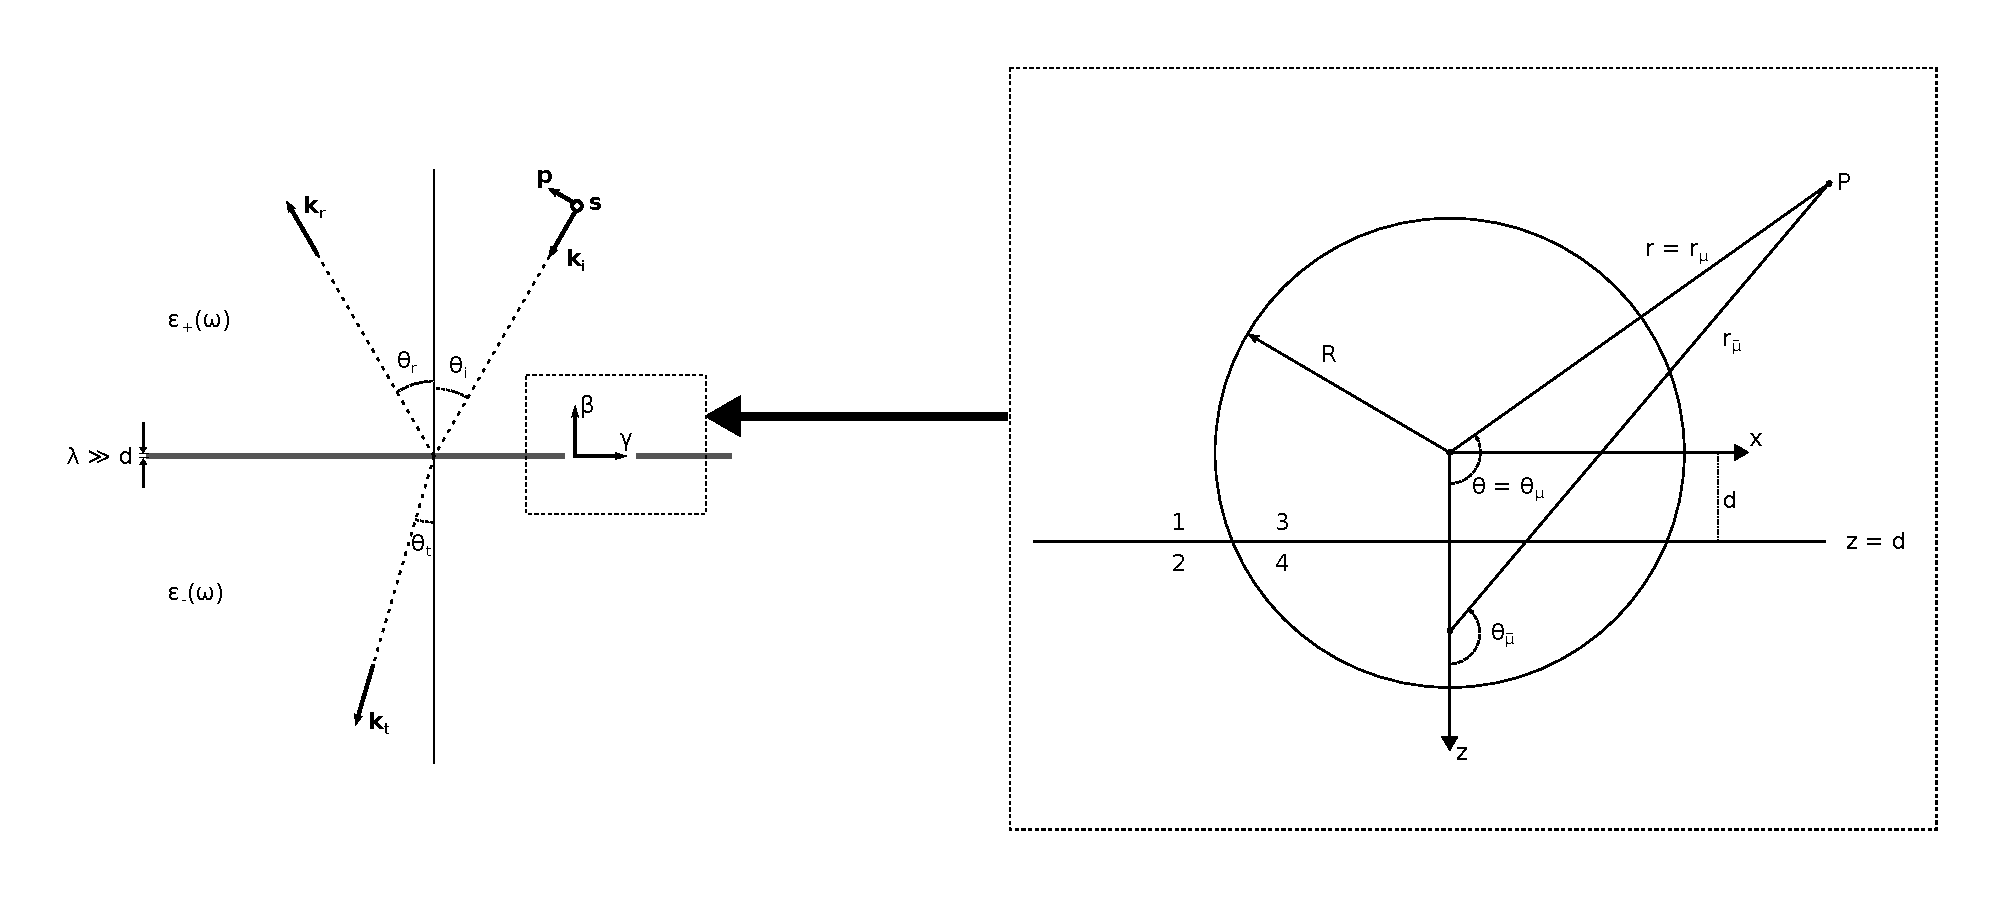
\includegraphics[width=1.0\textwidth]{Figures/filmGeometry.pdf}
   \caption{To the left: the transmission and reflection of a pertubed surface layer with thickness $d$, 
      which is assumed to be much smaller than the optical wavelength $\lambda$ of the incoming wave.
      The reflection and transmission amplitudes depend on the surface 
      susceptibilities. The first order surface susceptibilities, $\gamma$ and $\beta$, describe
      the ability of the surface to polarise in the parallel or perpendicular direction. These
      coefficients can be calculated from evaluating the geometry of the trunctated spheres
      (shown to the right), making up
      the granular thin film (\cite{Lazzari2002}, p.126). Adopted from (\cite{Lazzari2002}, p.125)
   }
   \label{fig:filmGeometry}
\end{figure}
%
The coordinate system for the expansion is given in Figure \ref{fig:filmGeometry}, with $\mu$ denoting 
the center of expansion, which may be centered at the truncated sphere or varied along the vertical
symmetry axis. To deal with the boundary truncating the sphere, the classical image technique is used 
%(\cite{Lazzari2002},(13)). 
\cite{Lazzari2002}.
This is done by having a image expansion center located at the opposite side of the surface,
compared to $\mu$, inside the substrate. The image expansion point is denoted by $\bar{\mu}$. 
%%
%\textbf{Should I also mention $t_r$ and the difference between $t_r > 0$ and $t_r < 0$?}
%%
As shown in Figure \ref{fig:filmGeometry}, mathematical approach assumes 4 different media,
even though region 4 is part of the substrate. When specifying the material in the software
region 2 and 4, which constitute the substrate, are usually set to be the same.
Using Eq.\eqref{multipoleSolution} to expand the potential around the expansion center and 
the image, the potential in the different regions take the form:
%
\begin{subequations}
\label{multExp}
\begin{align}
   &\Psi_1(\boldsymbol{r}) = \Psi_i(\boldsymbol{r}) + \sum\limits_{lm}^{l \neq 0} A_{lm} r_{\mu}^{-l-1} Y_l^m(\theta_{\mu},\phi_{\mu})
   + \sum\limits_{lm}^{l \neq 0} A^r_{lm} r_{\bar{\mu}}^{-l-1} Y_l^m(\theta_{\bar{\mu}},\phi_{\bar{\mu}})
   \label{multExp1}\\
%
   &\Psi_2(\boldsymbol{r}) = \Psi_t(\boldsymbol{r}) + \sum\limits_{lm}^{l \neq 0} A_{lm}^t r_{\mu}^{-l-1} Y_l^m(\theta_{\mu},\phi_{\mu})
   \label{multExp2}\\
%
   &\Psi_3(\boldsymbol{r}) = \psi_0(\boldsymbol{r}) + \sum\limits_{lm}^{l \neq 0} B_{lm} r_{\mu}^l Y_l^m(\theta_{\mu},\phi_{\mu})
   + \sum\limits_{lm}^{l \neq 0} B^r_{lm} r_{\bar{\mu}}^l Y_l^m(\theta_{\bar{\mu}},\phi_{\bar{\mu}})
   \label{multExp3}\\
%
   &\Psi_4(\boldsymbol{r}) = \psi_0(\boldsymbol{r}) + \sum\limits_{lm}^{l \neq 0} B_{lm}^t r_{\mu}^l Y_l^m(\theta_{\mu},\phi_{\mu})
   \label{multExp4}
\end{align}
\end{subequations}
%
Here, the $r^l\big|_{l=0}$ terms of the expansion are constant and have been extracted, 
giving the value $\psi_0(\boldsymbol{r})$ inside the sphere, corresponding to region 3 and 4 
in Figure \ref{fig:filmGeometry}.
The negative terms $r^{-1-l}\big|_{l=0} = r^{-1}$ represents free charge, wich has been assumed to be
zero, and are removed \cite[p.~79]{BedeauxVliegerBook}. 
Outside the sphere, i.e. region 1 and 2, the potential is set to zero 
simply because the potential reference point can be chosen freely. 
In addition to the $l=0$-terms, the incident field gives rise to the potential $\Psi_i(\boldsymbol{r})$. 
Some of the incident light is transmitted directly into the substrate and the resulting scalar field
is given by $\Psi_t(\boldsymbol{r})$.
%
\textbf{Burde kanskje ta med at $\Psi_i(\boldsymbol{r})$, $\Psi_t(\boldsymbol{r}) \sim -\boldsymbol{r}\cdot\
\boldsymbol{E}_0$. Ref fra: \cite[p.~95]{BedeauxVliegerBook}}
%
Comparing Eqs. \eqref{multExp} to Eq. \eqref{multipoleSolution}, it is worth to note that all the
$r^l$-terms in region 1 and 2, $r^{-l-1}$-terms in region 3 and 4 are removed due to the divergence
of the potential as $r \rightarrow \infty$ and $r \rightarrow 0$, respectively.
\\
\\
The boundary conditions for the electric potential is given by \cite[p.~89-90]{Griffiths}
\begin{align}
   \varepsilon\!_i\!(\omega) \:\: \partial_n \Psi_i(\boldsymbol{r}) &= \varepsilon\!_j\!(\omega) \:\:\partial_n \Psi\!_j(\boldsymbol{r})
   &\Psi_i(\boldsymbol{r}) &=\Psi\!_j(\boldsymbol{r})
\end{align}
where $\partial_n = \hat{n} \cdot \nabla$ is the derivative with respect to the 
normal direction $\hat{n}$ to the boundary surface, and the indicies $i,j \in \{1,2,3,4\}$, $i \neq j$
denotes the different media included at the different boundaries.
%
From the boundary conditions, handled by the method of images \cite[p.~121]{Griffiths},
the relation between the multipole coefficients are found
%
\begin{subequations}
\label{multExpCoeff1}
\begin{align}
   A^r_{lm} & = (-1)^{l+m} \frac{\varepsilon_1 - \varepsilon_2}{\varepsilon_1 + \varepsilon_2} A_{lm}
   \label{multExpCoeffAr}\\
%
   A^t_{lm} & = \frac{2\varepsilon_1}{\varepsilon_1 + \varepsilon_2} A_{lm}
   \label{multExpCoeffAt}
\end{align}
\label{multExpCoeff2}
\begin{align}
   B^r_{lm} & = (-1)^{l+m} \frac{\varepsilon_3 - \varepsilon_4}{\varepsilon_3 + \varepsilon_4} B_{lm}
   \label{multExpCoeffBr}\\
%
   B^t_{lm} & = \frac{2\varepsilon_3}{\varepsilon_3 + \varepsilon_4} B_{lm}.
   \label{multExpCoeffAt}
\end{align}
\end{subequations}
%
However, there are still 4 unknowns for each multipole order, i.e. for every configuration of $l$ and $m$.
By using the orthogonality of the spherical harmonics $Y_l^m(\theta,\phi)$ to treat the boundary
of the sphere, called the weak formulation of the boundary conditions, give two infinite linear 
systems for the multipolar coefficients $A_{lm}$ and $B_{lm}$ for $l = 1$, $m = 0, \pm 1$.
To solve this system in practive, some cut-off value $l = M$ for the expansion is set. 
Based on investigations by Simonsen and Lazzari \cite{Simonsen2000}
a truncation at $M = 16$ appeared to be sufficient in most cases. This result is based on 
post-checking the boundary condition for the potential and the normal displacement at the surface;
and convergence tests of the first term of the multipolar expansion. Keep in mind, that for 
cases like spherical caps (truncated at the upper hemisphere) or entire spheres on top of a substrate
the convergence could be slower, requiring a truncation $M>16$.
Finally, knowing the first multipolar coefficients the polarizability of the islands can be found
\begin{align}
   \alpha_{\perp} &\simeq A_{10}          &\alpha_{\parallel} &\simeq A_{11}.
\end{align}
The first $l=0$ terms of region 1 $A_{lm}$ are representing the dipole contribution, which dominates
in the far-field limit \cite[p.~99]{BedeauxVliegerBook} 

\subsection{Inter-island coupling; collective contribution}
So far, the discussion has only included the response of a single island and would perhaps 
give resonable result in the low coverage limit. However, this would lead to 
an increase in error for larger covarages and create the need for a correction
due to the increasing island-island interaction for higher coverages
\cite[p.~20]{Lie2010}.
%
%?????????????????????????????????????????? 
\textbf{ <- Can I use this???????????????}.% the lie referance (it's to the master thesis)
%??????????????????????????????????????????
%
By assuming that the island are sufficiently close to one another such that their mutual separation is 
negligible compared to the optical wavelength, a correction to the low-coverage result can be obtained. 
In this limit, the islands would be excited by the same incident field and have similar responses
to the field. See Figure \ref{fig:quasiStatic}.
%
\begin{figure}
    \centering
    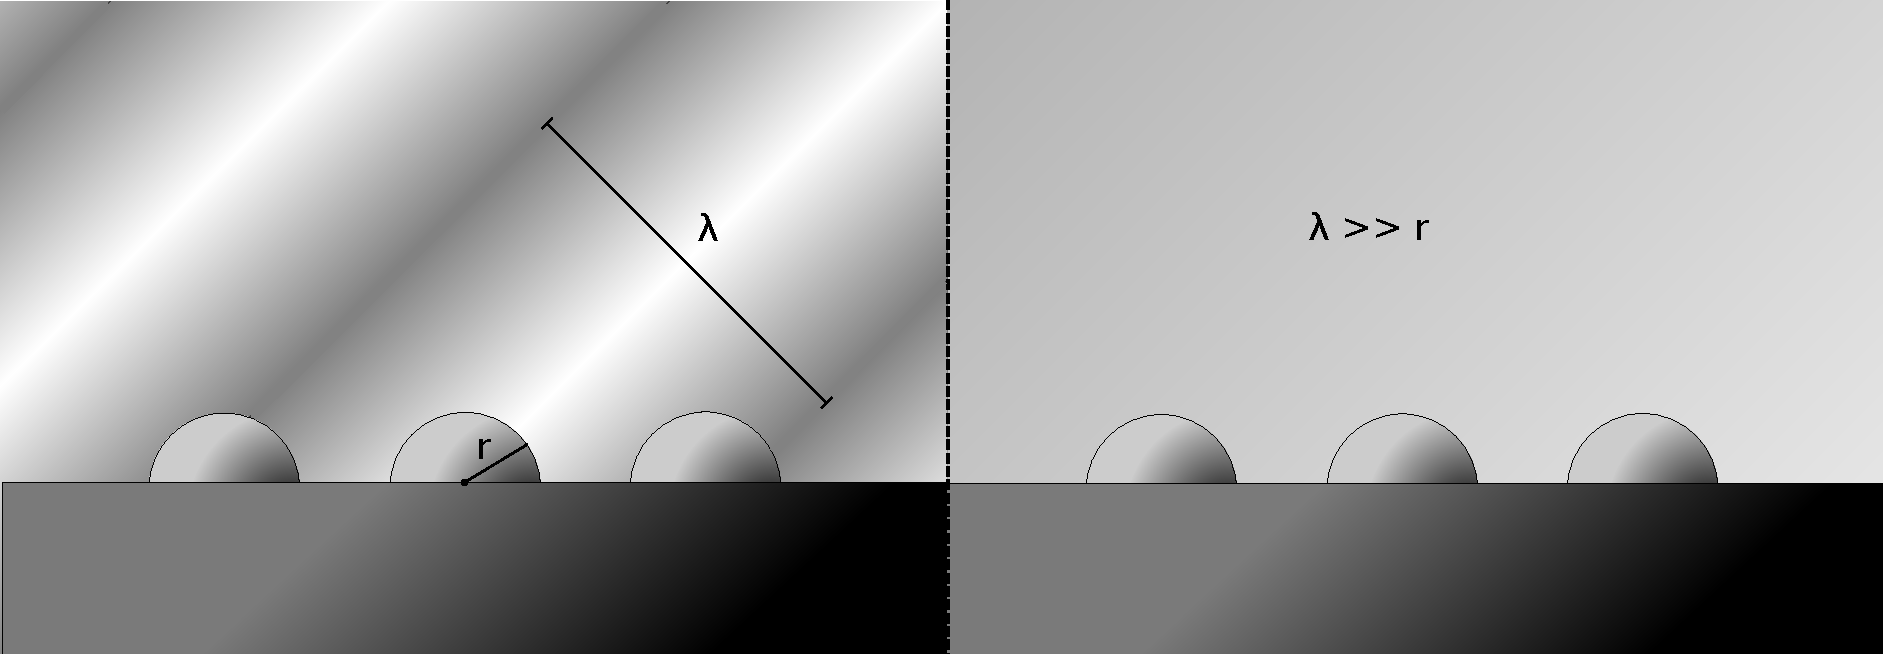
\includegraphics[width=1.0\textwidth]{Figures/quasiStaticApprox3.pdf}
    \caption{
       When the size and separation of the particles are small compared to the optical wavelength
       of the incident electromagnetic wave the particles are approximately excited by the same field.
       Here the greyscale of the background represent the amplitude of the field.
    }
    \label{fig:quasiStatic}
\end{figure}
%
Assuming a dipole response, the islands would be affected by the dipole
fields excited in the neighboring particles. If the spheres are truncated by the substrate through their
lower hemisphere, the modified polarizabilities compared to the isolated polarizatilities, $\alpha_{\perp},
\alpha_{\parallel}$, become \cite[p.~181]{BedeauxVliegerBook}
\begin{align}
   \alpha^{\text{mod}}_{\perp} &= \frac{\alpha_{\perp}}{ 1 - 2 \alpha_{\perp} I_{\perp}^{20} }
   &\alpha^{\text{mod}}_{\parallel} &= \frac{\alpha_{\parallel}}{ 1 + 2 \alpha_{\parallel} I_{\parallel}^{20}}.
\end{align}
%
The defined functions in the correction are called the interaction functions \cite{Lazzari2002}
%
\begin{subequations}
\label{couplingPolarizability}
\begin{align}
I_{\perp}^{20} = \frac{1}{\sqrt{20\pi} L^3 \varepsilon_{_-} } 
   \Bigg[
   S_{20} - \Bigg( \frac{\varepsilon_{_-}-\varepsilon_{_+}}{\varepsilon_{_-}+\varepsilon_{_+}} \Bigg) 
   \tilde{S}_{20}^r
   \Bigg]
   \label{couplingPolarizability1}\\
%
   I_{\parallel}^{20} = \frac{1}{\sqrt{20\pi} L^3 \varepsilon_{_-} } 
   \Bigg[
   S_{20} + \Bigg( \frac{\varepsilon_{_-}-\varepsilon_{_+}}{\varepsilon_{_-}+\varepsilon_{_+}} \Bigg) 
   \tilde{S}_{20}^r
   \Bigg],
   \label{couplingPolarizability2}
\end{align}
\end{subequations}
%
where
%
\begin{subequations}
\label{latticeSums}
\begin{align}
   S_{20} = \sum\limits_{i \neq 0} \Bigg( \frac{L}{r}\Bigg)^3 Y_2^0 (\theta,\phi) \Biggr|_{r=R_i}
   \label{latticeSums1} \\
%
   S_{20}^r = \sum\limits_{i \neq 0} \Bigg( \frac{L}{r}\Bigg)^3 Y_2^0 (\theta,\phi) \Biggr|_{r=R_i^r}
   \label{latticeSums2}
\end{align}
\end{subequations}
%
are the direct and image lattice sums, describing the interaction with the other direct and 
image dipoles, respectively. $L$ stands for the lattice constant. The $i=0$ term in the summation
gives the contribution from the interaction with the corresponding image of an island. This 
is taken into account when calculating the isolated response and is therefore not needed in
Eq.\eqref{latticeSums}. 
The validity of the dipolar approximation was tested by Lazzari and Simonsen
for hemispherical silver islands layed out in a hexagonal pattern on a MgO substrate
\cite[p.~129-130]{Lazzari2002} The polarizabilities were computed for $M = 16$ 
and showed that the relative error of the dipole approximation compared quadrupole approximation is
$sim 1\%$ up to 40\% coverage, which is higher than the interesting limits encountered in 
experiments.




















%












%\textbf{From ''GranFilm-Software-Article''}: \\
%Information on the dieletric behavior of surfaes can often be obtained by measuring the Fresnel coefficients,
%such as reflection, transmission and absorption. \\
%?p.2?: for a layer with thickness negligible compared to wavelength, we introduce surface susceptibilities 
%which interconnect the  fresnel coeff. and characterise the optical response of the surface. ?? DID I UNDERSTAND THIS CORRECTLY? ?? \\
%Since all the Fresnel coeff. can be expressed in terms of these surface susceptibilities, the main task consist of calculating these coefficients for the appropriate geometry. \\
%\textbf{Goal of GranFilm:} to calculate ?surface-susceptibility-/fresnel-coefficients? and the associated measurableFresnel quantities for various surface layer geometries. 
%\begin{itemize}
%\item GranFilm is free open-source software
%\end{itemize}
%\subsection{Mie resonances/ plasmon absorption modes}
%\textbf{From ''GranFilm-Software-Article''}: \\
%when small metallic particles, the resonances can be absorbed by visible light and strongly affect the fresnel 
%coefficients depending on the particle morphology.
%%
%\subsection{Quasistatic Approximation}
%%
%\subsection{Electromagnetic excess fields }
%%
%\textbf{From ''GranFilm-Software-Article''}: \\
%(Bedeaux and Vlieger) \\
%Difference between the bulk extrapolated fields and the real fields. The BC at the dividing surface
%(which drive all fresnel coeff.) are given in terms of the integrated excess fields perpendicular to
%the surface. \\
%Bedeaux and Vlieger $\rightarrow$ formalism of excess quantities (does not require exact knowledge of the near suface EM-field behaviour). \\
%Excess fields are defined as the differene between the real fields and the bulk fields extrapolated to the surface. E.g. for the electric field $E(r)$ the excess quantity is defined as
%\begin{align}
   %E_{ex} (r) = E(r) - E^-(r) \theta(-z) - E^+(r)\theta(z),
%\end{align}
%where $\theta(z)$ is the Heaviside function and the superscript $\pm$ are used to indicate the region above (+) and below (-) the dividing interface at $z = 0$. 
%The excess field is only significant close to the surface, since $E(r, \omega) \rightarrow \rightarrow E^{\pm}(r,\omega)$  for $z \rightarrow \pm \infty$. \\
%\textit{QUESTION: \@ Is the $E^{\pm}$ field solved for a infinite homogeneous medium of type (+) and (-) respectively  OR the field in simple two media interface scattering?} \\
%\textbf{From Leif Amund Lies Msc Thesis}: \\
%Since the excess fields will only be significant close to the surface, they may be thought of as perturbations to the simple case of flat interface. 
%\textit{OWN INTERPRETATION: \@ This meas that the bulk fields are the fields created from scattering in the interface between two half-infinite media.} \\
%Instead of tediously using the quasi-static-"no source"-BC, the excess fields defined as for the electric field above are inserted into the full Maxwell equations to derive new non-sharp boundary conditions.
%The result reads
%%
%\textbf{From Leif Amund Lies Msc Thesis AND GranFilm-Article}: \\










\begin{thebibliography}{9}

      \bibitem{Lazzari2002}
      Lazzari R, Simonsen I. 
      GranFilm: a software for calculating thin-layer 
      dielectric properties and Fresnel coefficients.
      Thin Solid Films 
      2002;419:124-136
      \textit{ER DETTE RIKTIG?}

      \bibitem{Griffiths}
      Griffiths DJ.
      Introduction to electrodynamics, third edition.
      Pearson, international edition 2008.
      
      \bibitem{BedeauxVliegerBook}
      Bedeaux D, Vlieger J. 
      Optical properties of surfaces. 
      Imperial College Press, second edition 2004.

      \bibitem{Larsson2007}
      Larsson J.
      Electromagnetics from a quasistatic perspective.
      American Association of Physics Teachers, 2007.
      \textbf{??Er denne riktig???}

      \bibitem{Simonsen2000}
      Simonsen I, Lazzari R. Jupille J, Roux S.
      Numerical modeling of the optical response of supported metallic particles.
      Physical Review B, 61(11):7722-7733, 2000.


      \bibitem{LieMaster2010}
      Lie LA, Simonsen I.
      Optical properties of a thin film of coated, truncated spheres.
      NTNU 2010.
      Imperial College Press, second edition 2004.
      \textbf{?FJERN DENNE!}
\end{thebibliography}

\newpage
\section{Method}


\newpage
\section{Results}
The following simulations are done with an incident plane wave of direction 
$(\theta_i,\phi_i) = (45^{\circ},0^{\circ})$, on VO$_2$ particles supported by a SiO$_2$ substrate
with truncation ratio $t_r = 0$. The surrounding medium is air with $\varepsilon(\omega,T) = 1$.
The particles are arranged in a square lattice with lattice constant $L = 45$nm and the
particle-particle interaction is given by a dipole contribution. The multipole truncation
is set to $M = 16$.
\section{Simulation 1; $R = 10$nm, p-polarized incident light}
%
\begin{figure}
    \centering
    \begin{subfigure}[b]{0.49\textwidth}
        \centering
        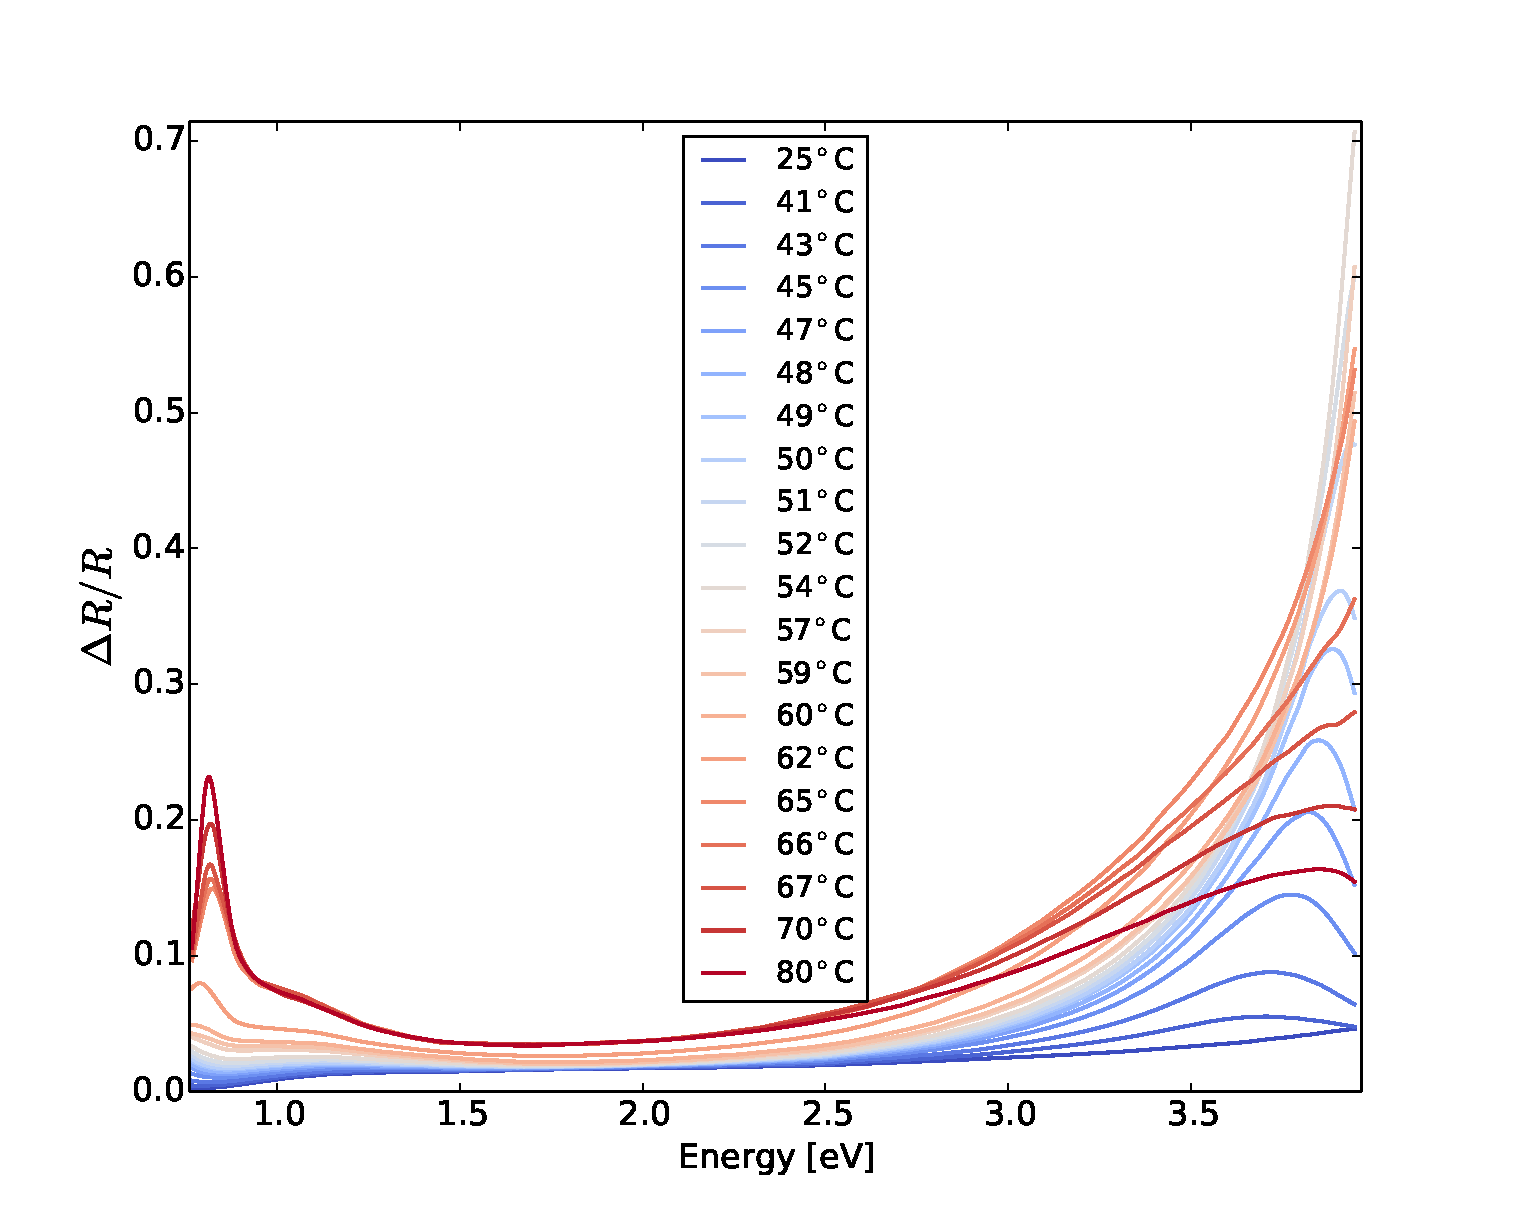
\includegraphics[width=\textwidth]{Results/Sim1/dR.pdf}
        \caption{}
        \label{fig:}
    \end{subfigure}
    %\hfill
    \begin{subfigure}[b]{0.49\textwidth}
        \centering
        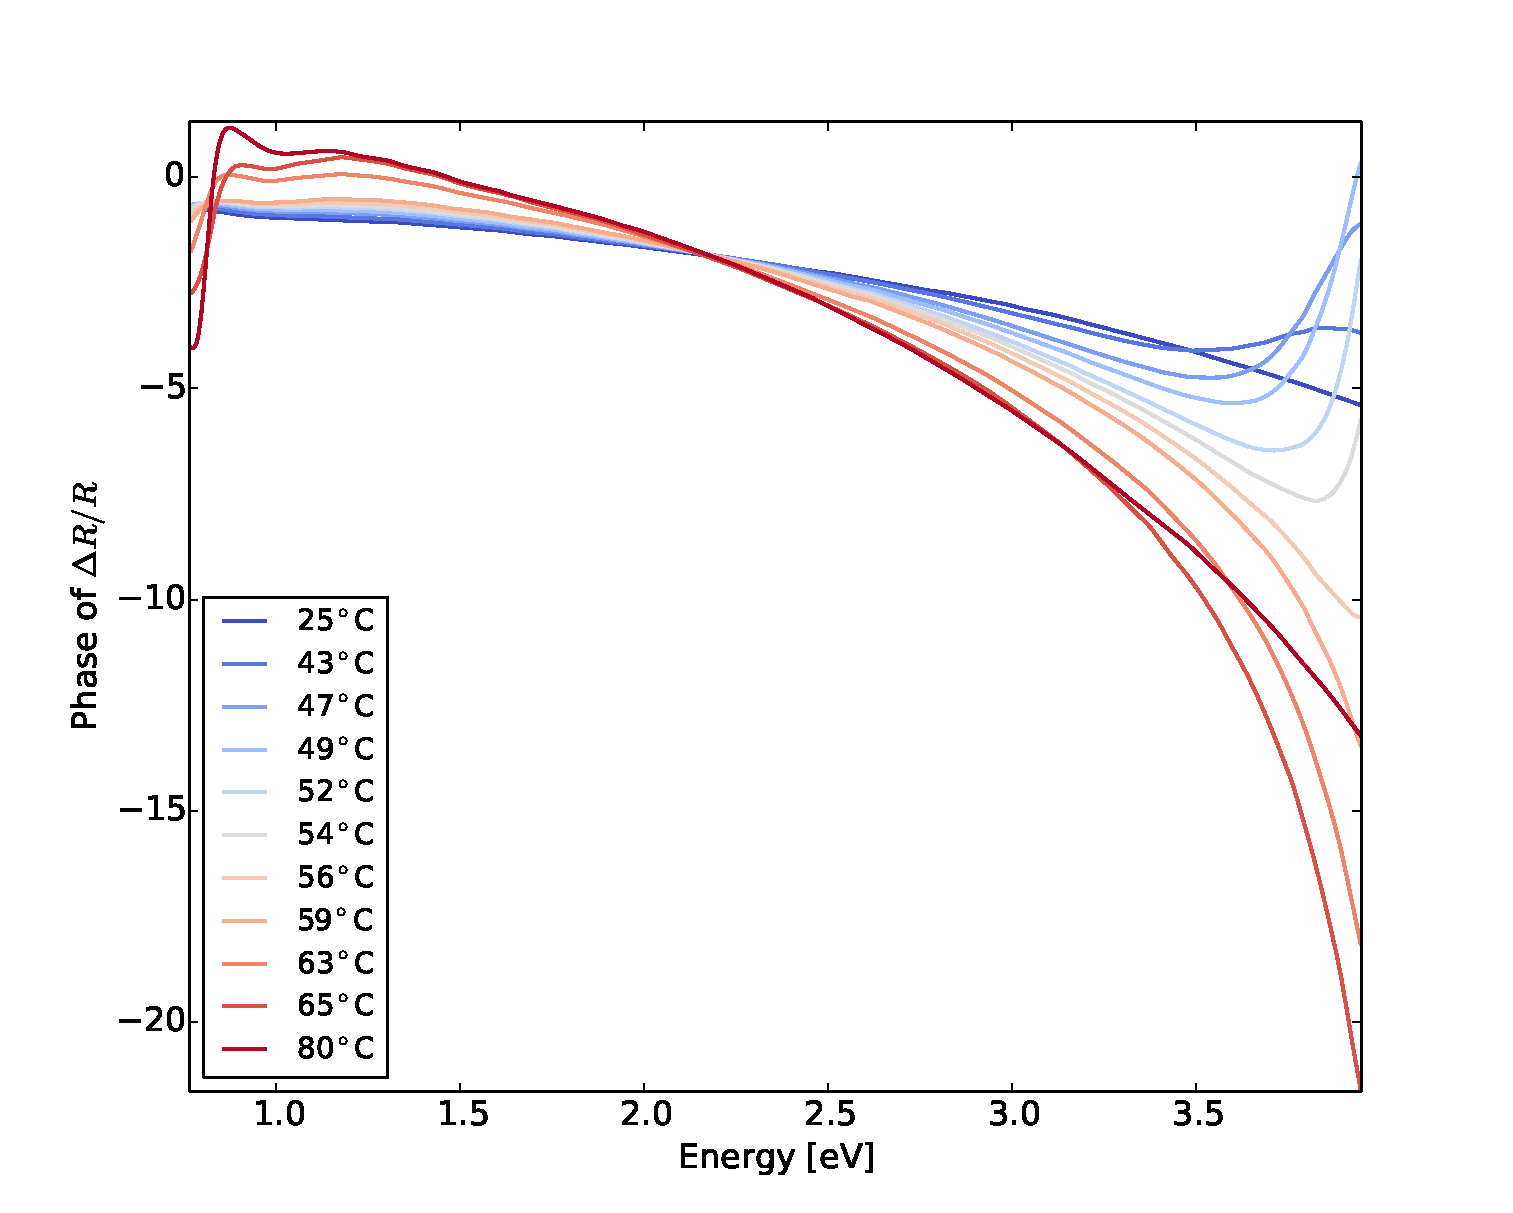
\includegraphics[width=\textwidth]{Results/Sim1/dRphase.pdf}
        \caption{}
        \label{fig:}
    \end{subfigure}
    \caption{Relative reflectance $\Delta R/R$}
    \label{fig:1}
\end{figure}
%
%
\begin{figure}
    \centering
    \begin{subfigure}[b]{0.49\textwidth}
        \centering
        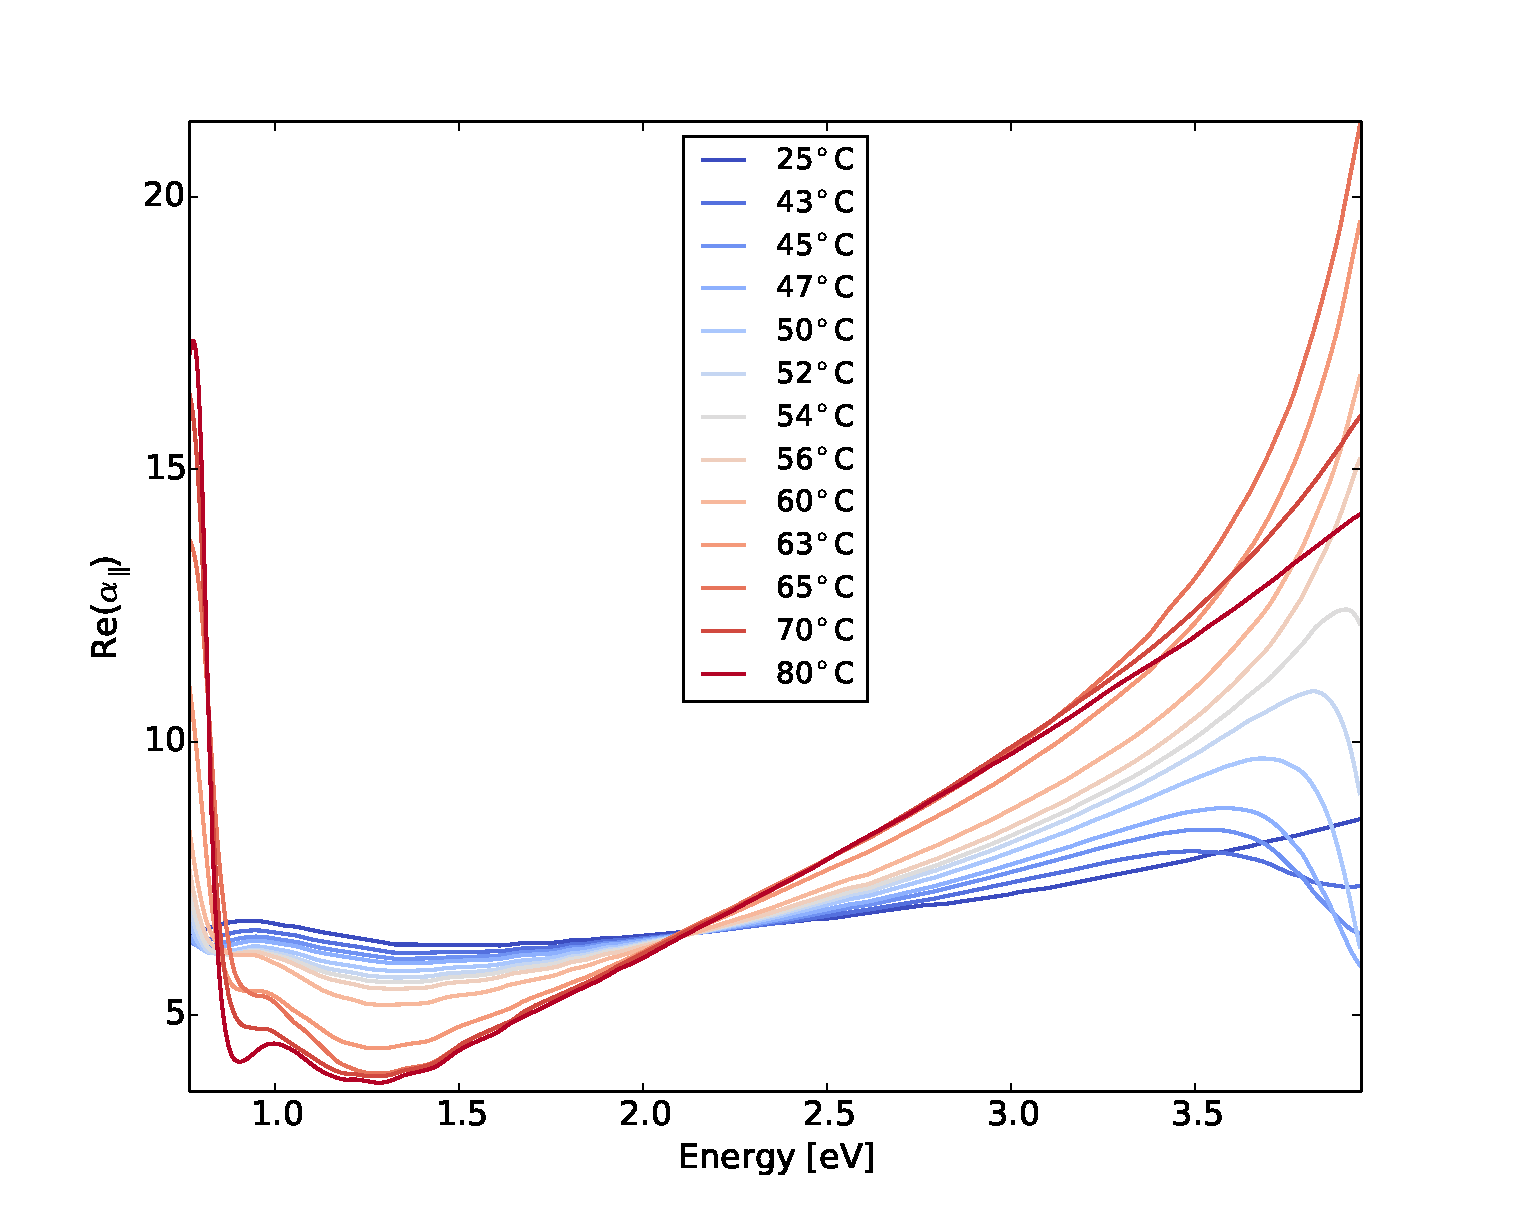
\includegraphics[width=\textwidth]{Results/Sim1/re_alpha_parallel.pdf}
        \caption{}
        \label{fig:2}
    \end{subfigure}
    %\hfill
    \begin{subfigure}[b]{0.49\textwidth}
        \centering
        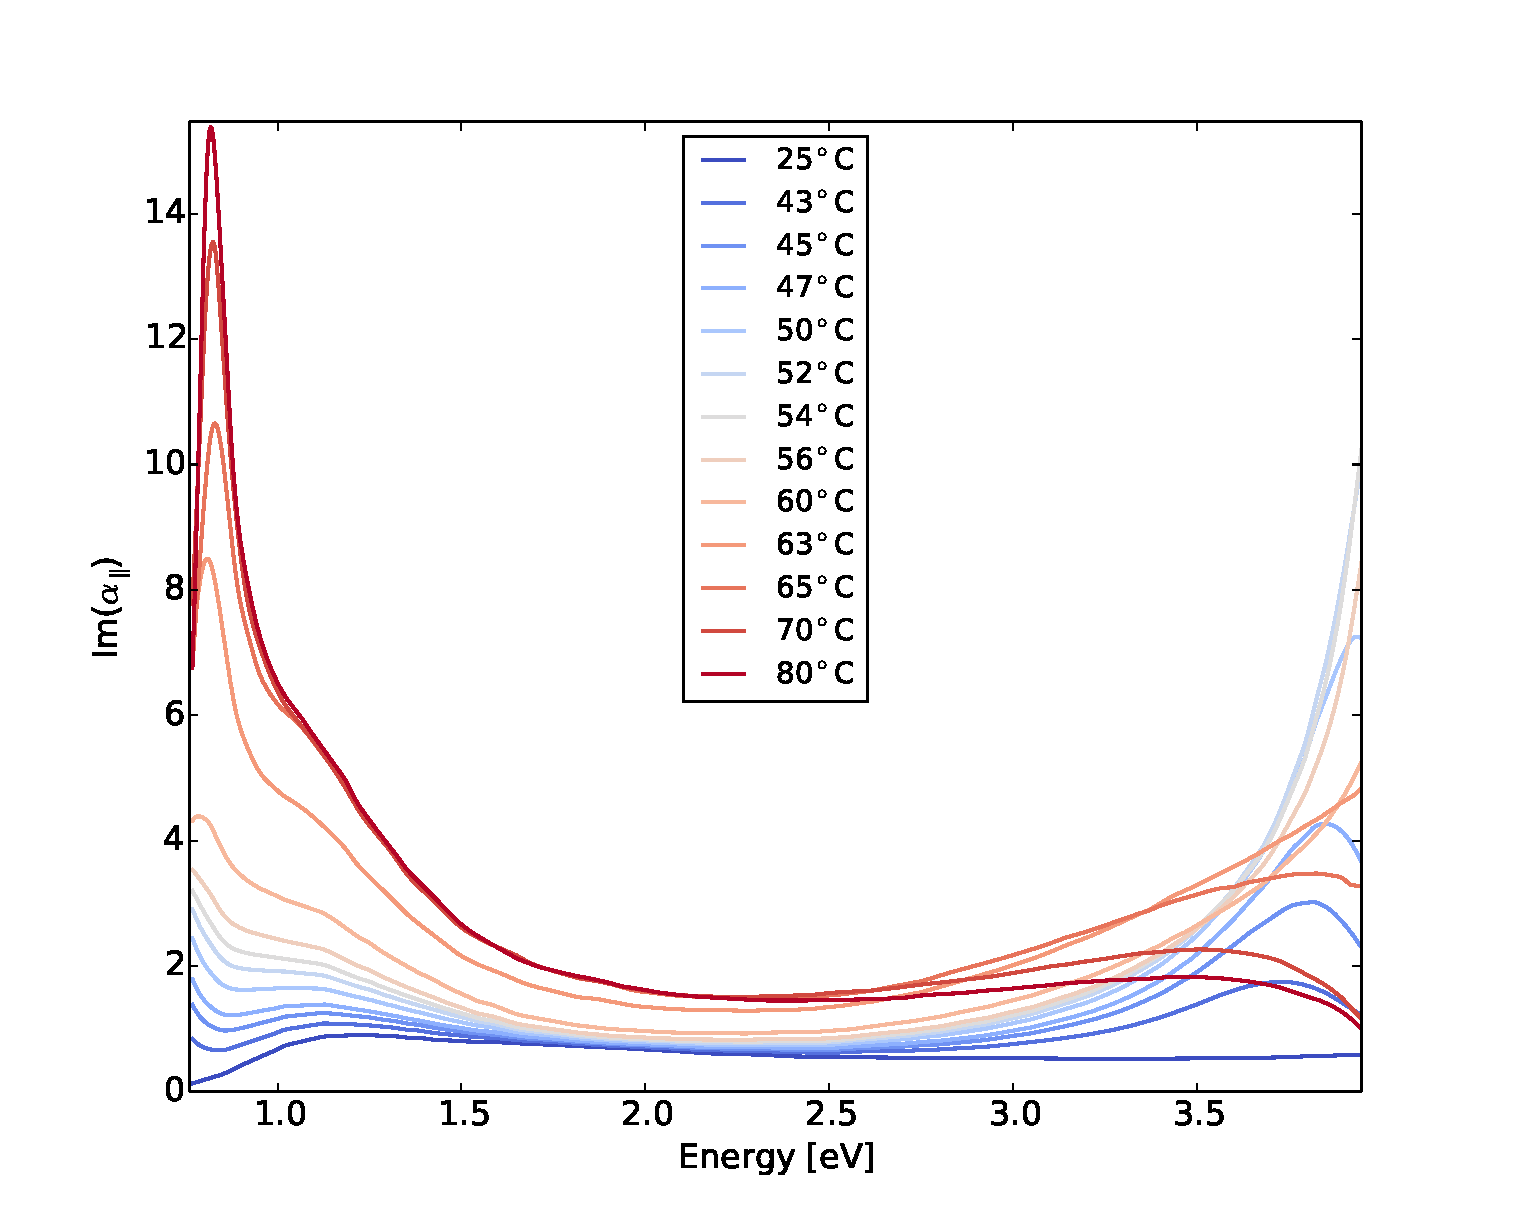
\includegraphics[width=\textwidth]{Results/Sim1/im_alpha_parallel.pdf}
        \caption{}
        \label{fig:2}
    \end{subfigure}
    %\hfill
    \begin{subfigure}[b]{0.49\textwidth}
        \centering
        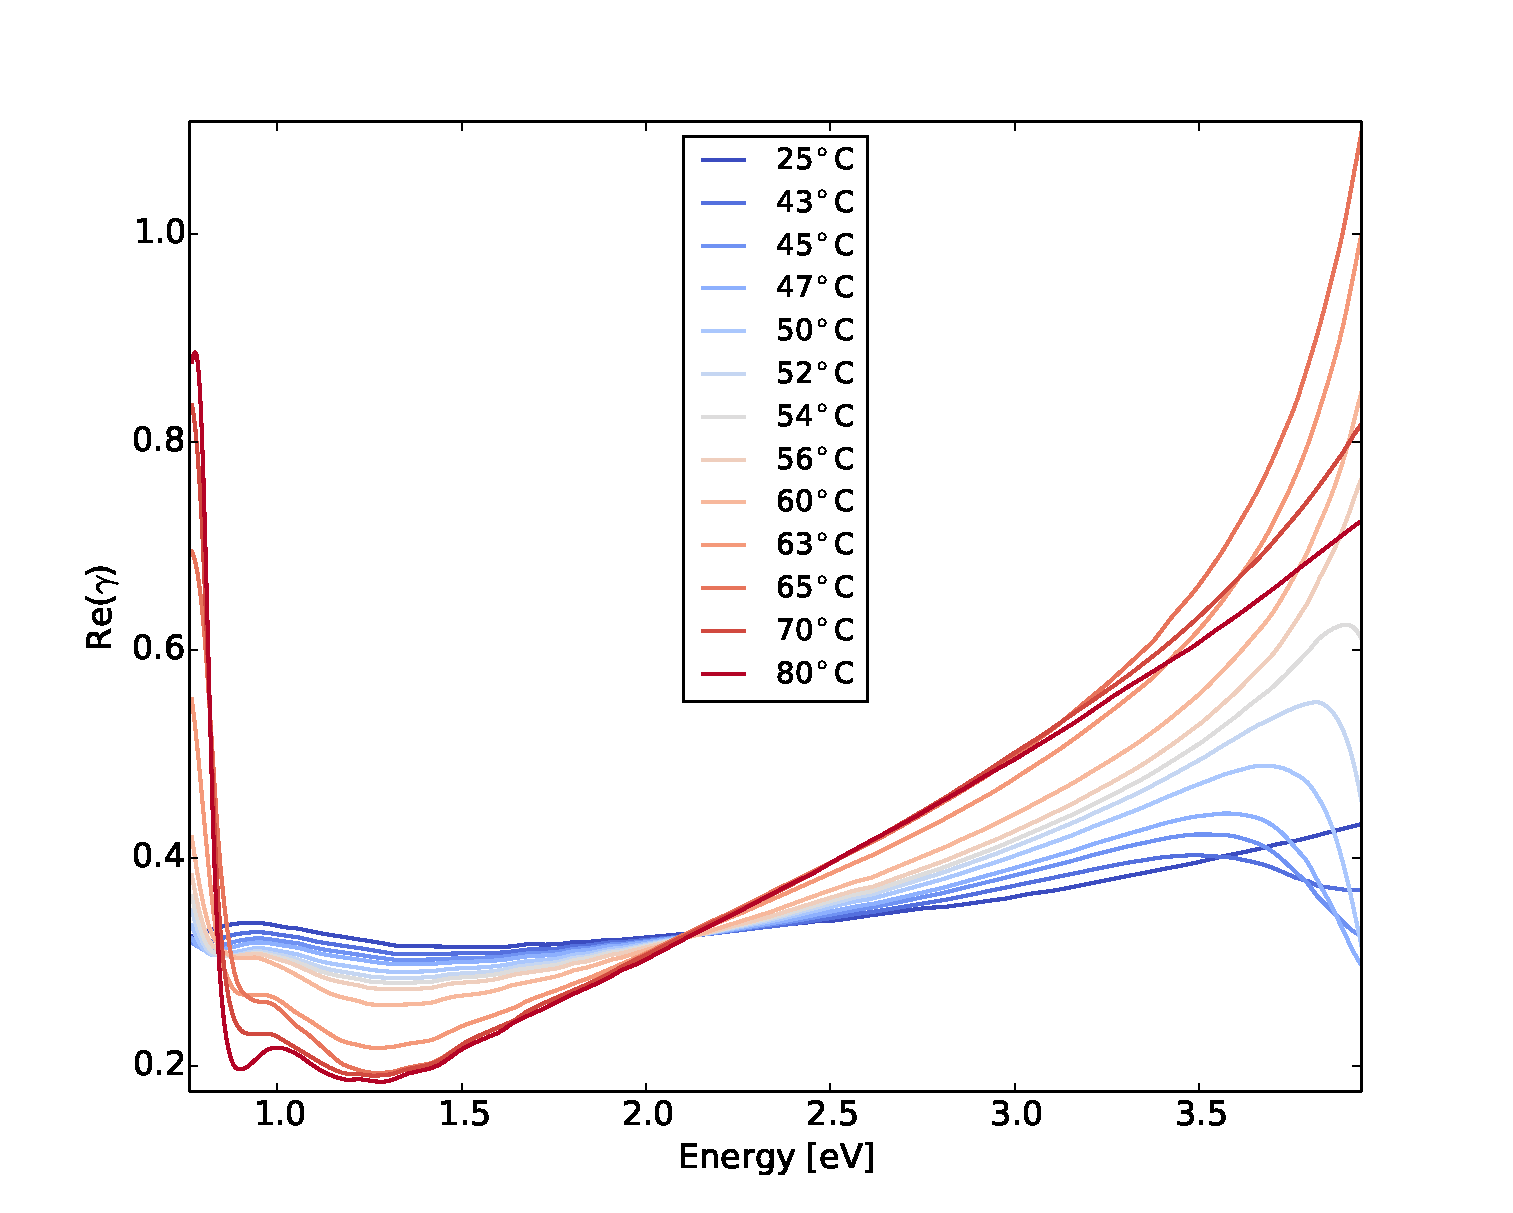
\includegraphics[width=\textwidth]{Results/Sim1/re_gamma.pdf}
        \caption{}
        \label{fig:2}
    \end{subfigure}
    %\hfill
    \begin{subfigure}[b]{0.49\textwidth}
        \centering
        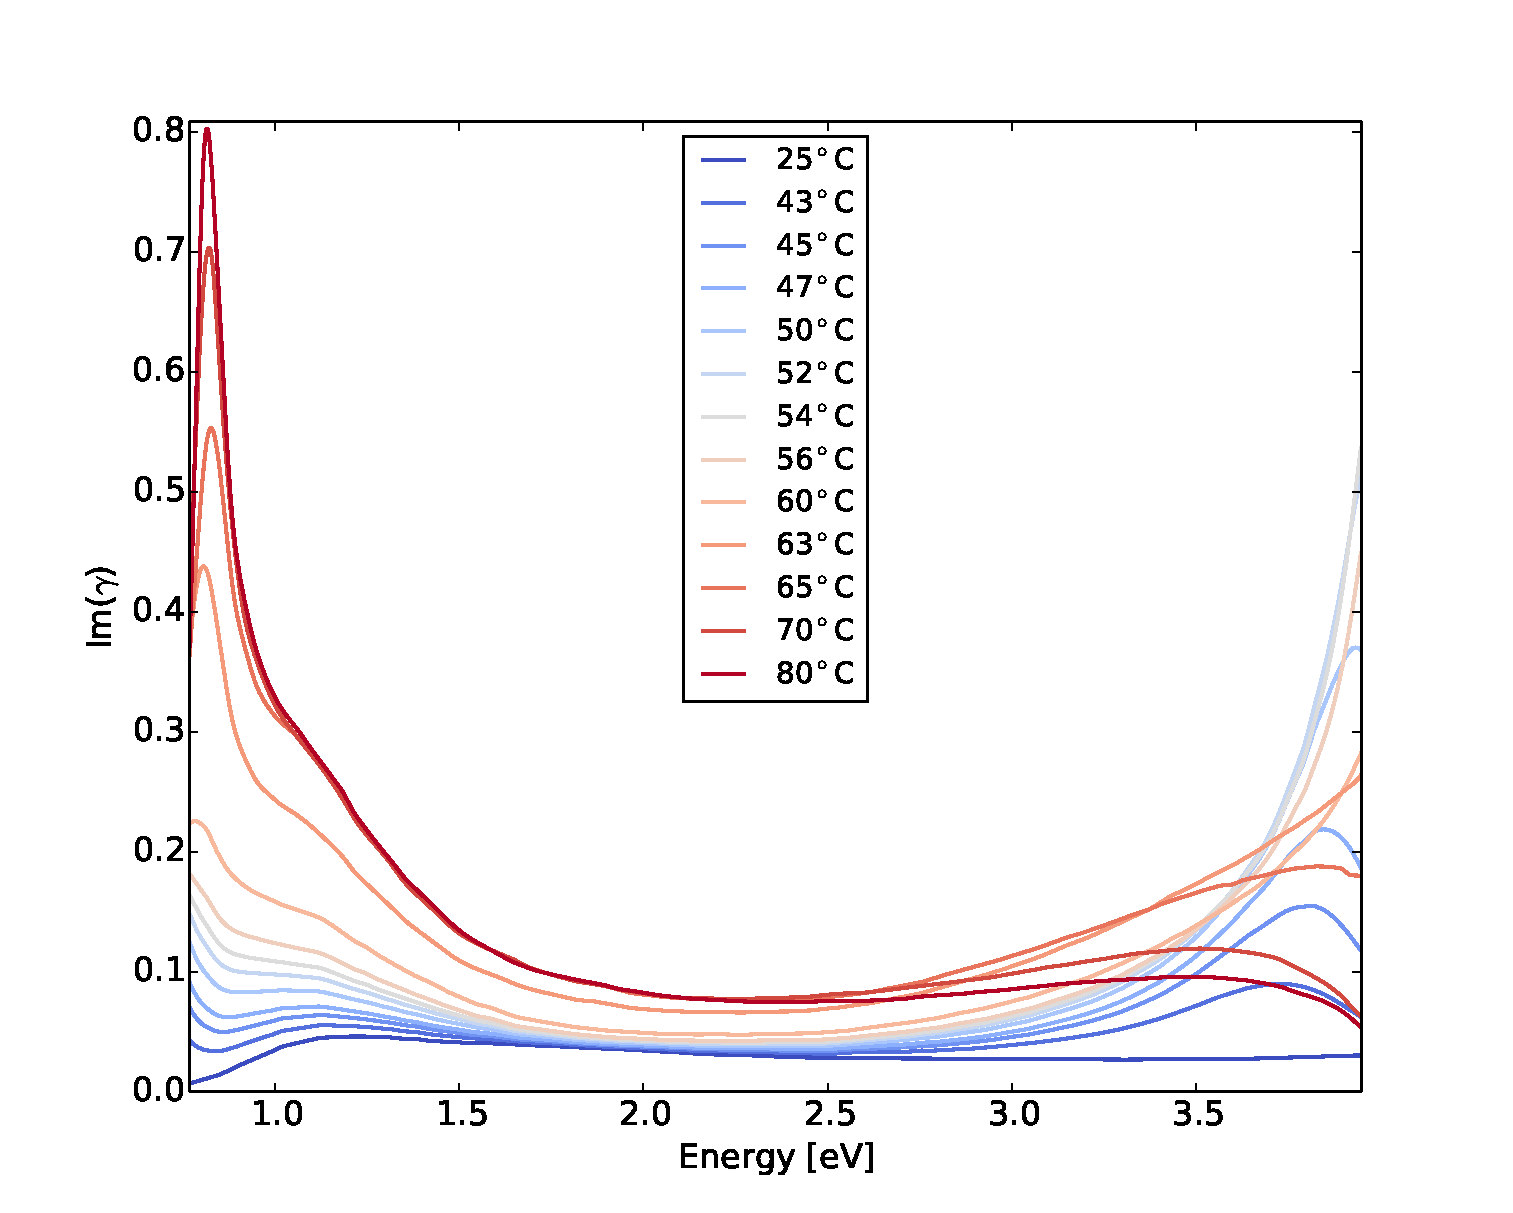
\includegraphics[width=\textwidth]{Results/Sim1/im_gamma.pdf}
        \caption{}
        \label{fig:2}
    \end{subfigure}
    \caption{Relative reflectance $\Delta R/R$}
    \label{fig:}
\end{figure}
%
%
\begin{figure}
    \centering
    \begin{subfigure}[b]{0.49\textwidth}
        \centering
        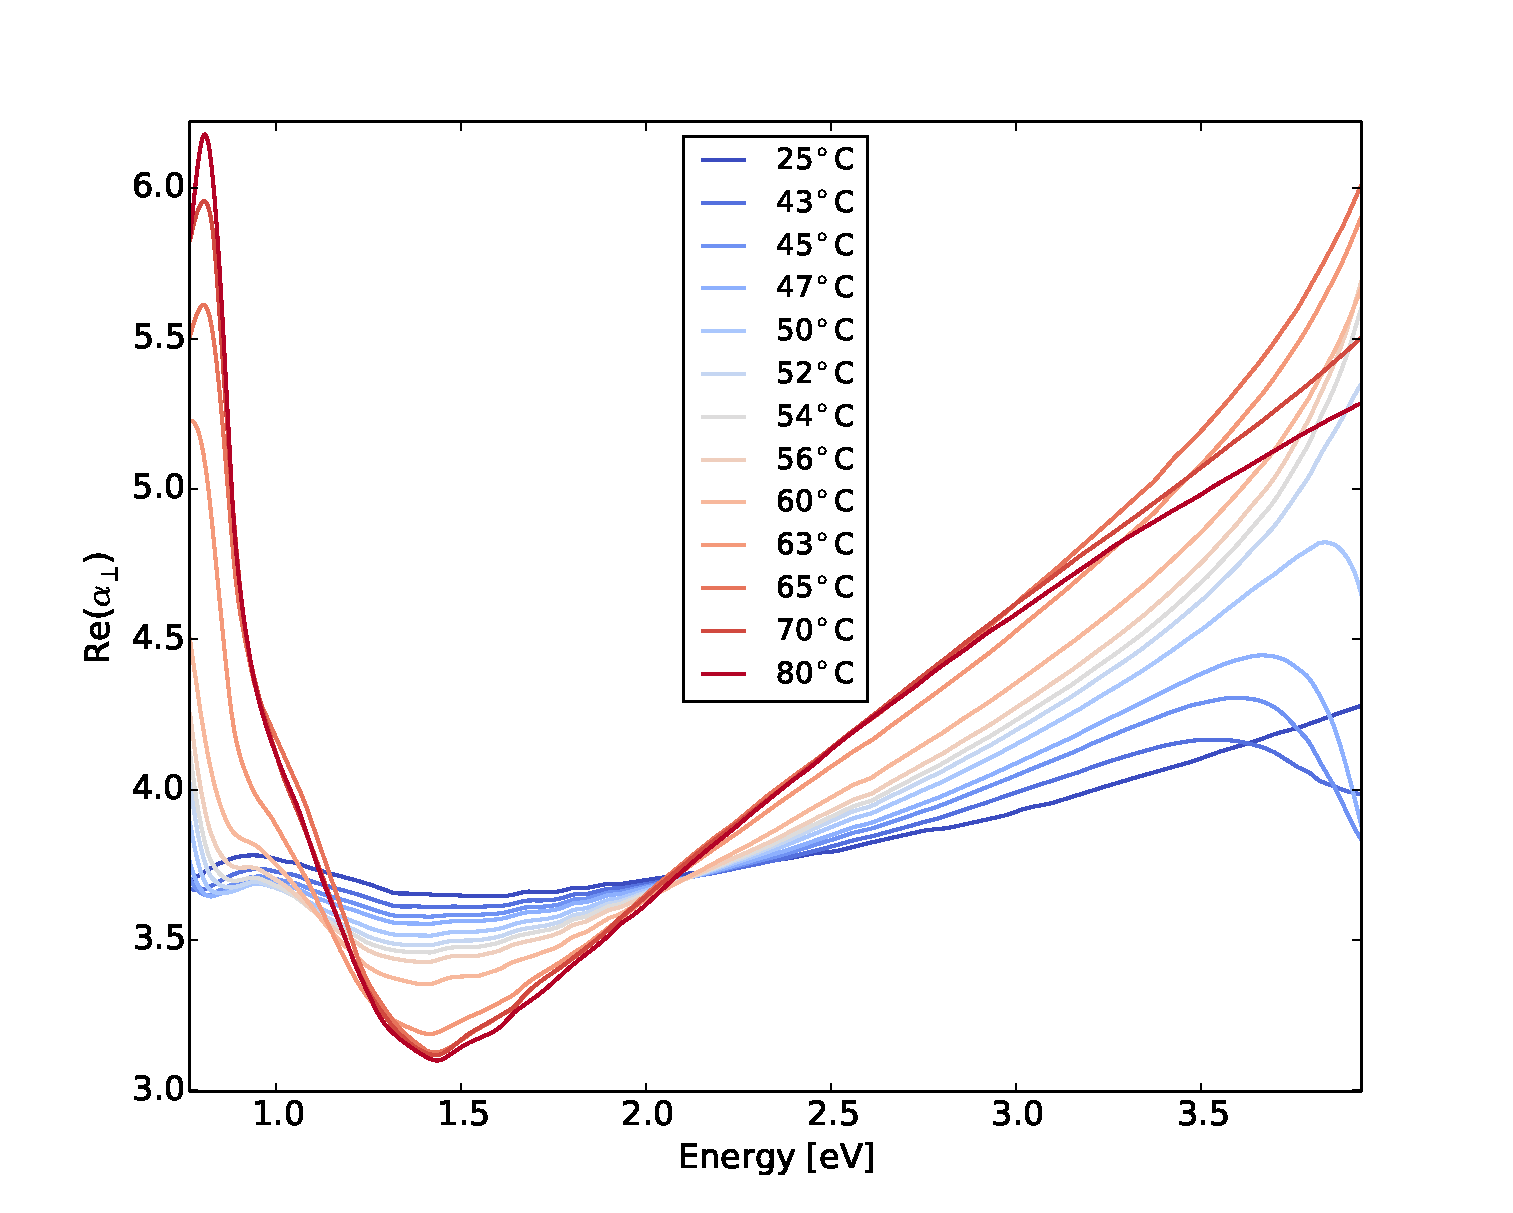
\includegraphics[width=\textwidth]{Results/Sim1/re_alpha_perp.pdf}
        \caption{}
        \label{fig:}
    \end{subfigure}
    %\hfill
    \begin{subfigure}[b]{0.49\textwidth}
        \centering
        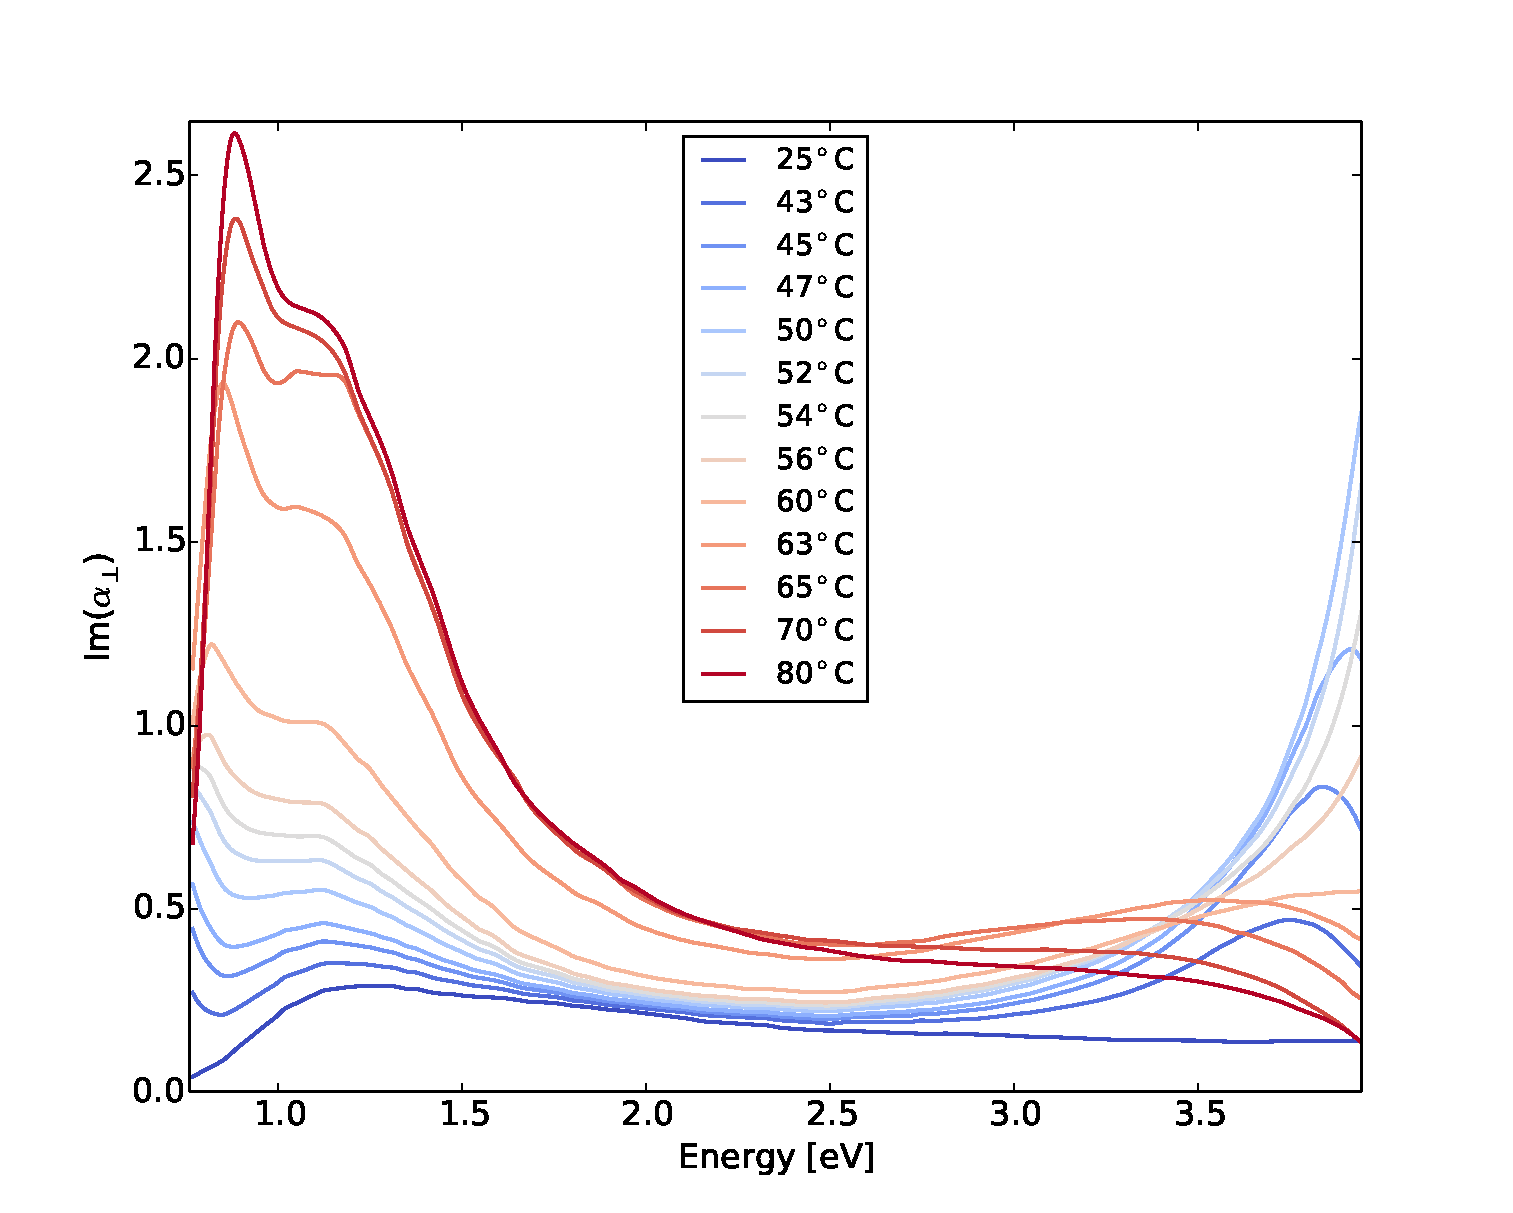
\includegraphics[width=\textwidth]{Results/Sim1/im_alpha_perp.pdf}
        \caption{}
        \label{fig:}
    \end{subfigure}
    %\hfill
    \begin{subfigure}[b]{0.49\textwidth}
        \centering
        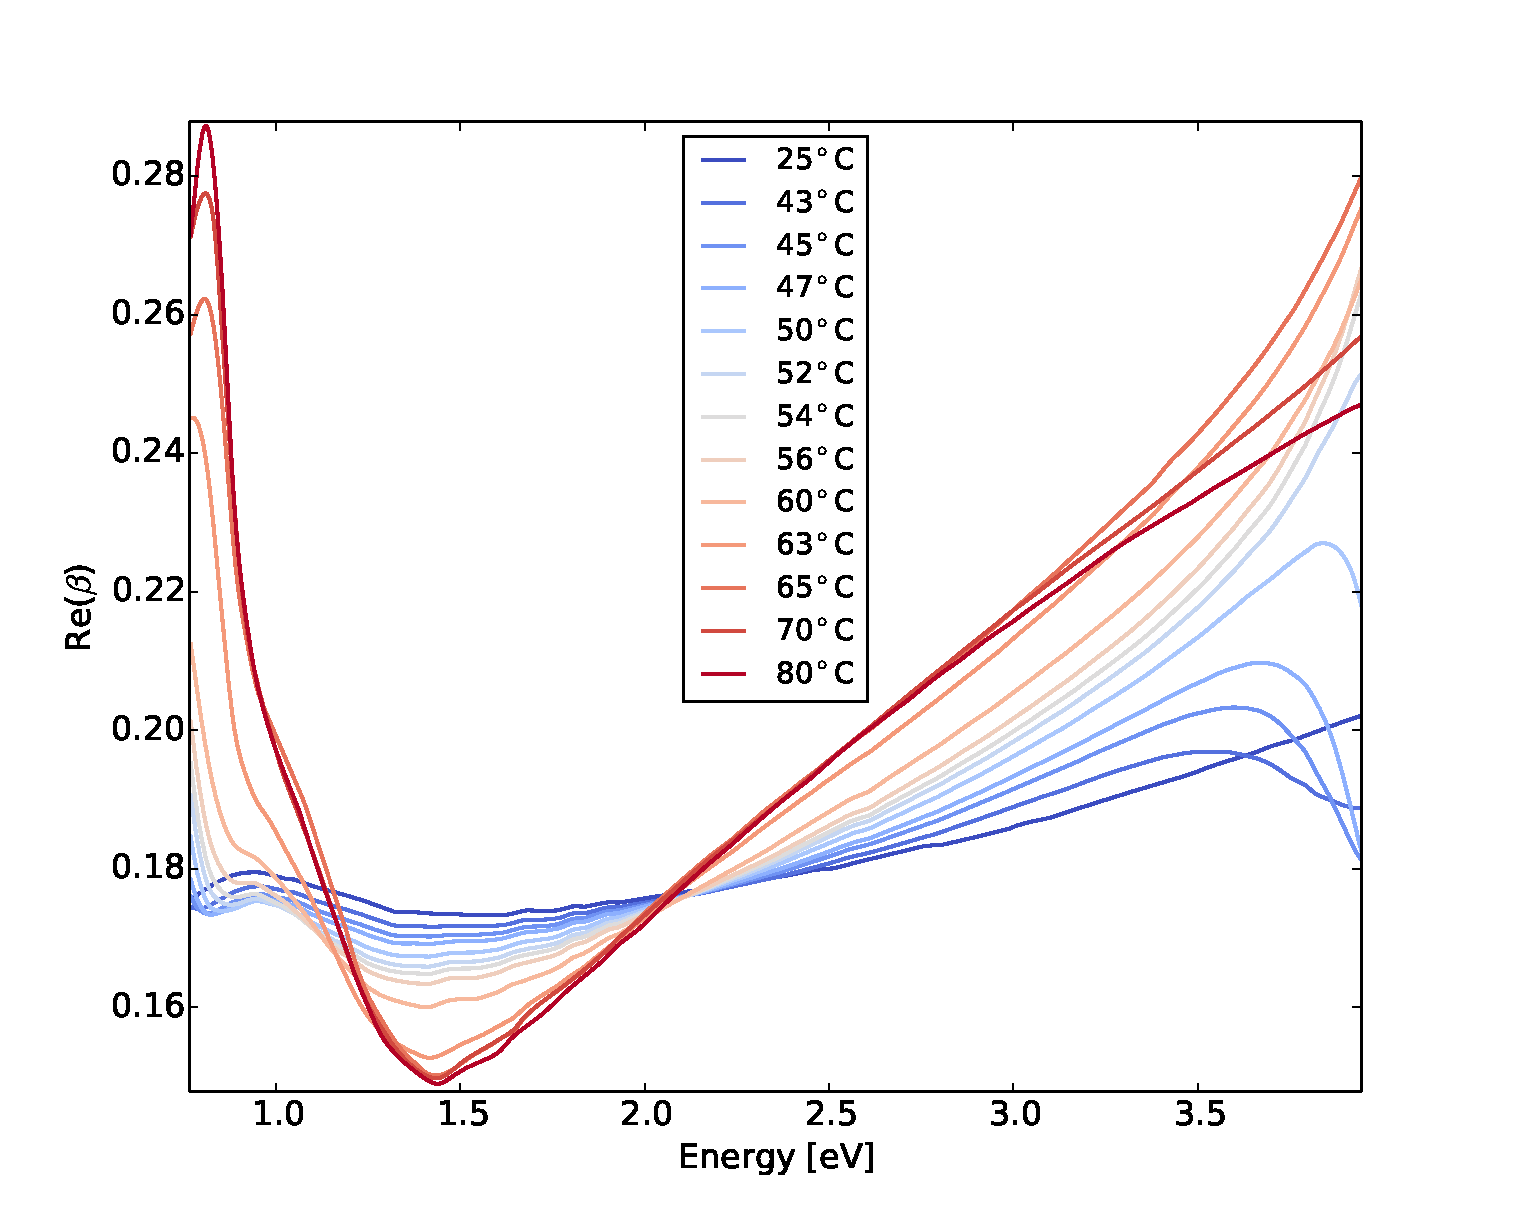
\includegraphics[width=\textwidth]{Results/Sim1/re_beta.pdf}
        \caption{}
        \label{fig:2}
    \end{subfigure}
    %\hfill
    \begin{subfigure}[b]{0.49\textwidth}
        \centering
        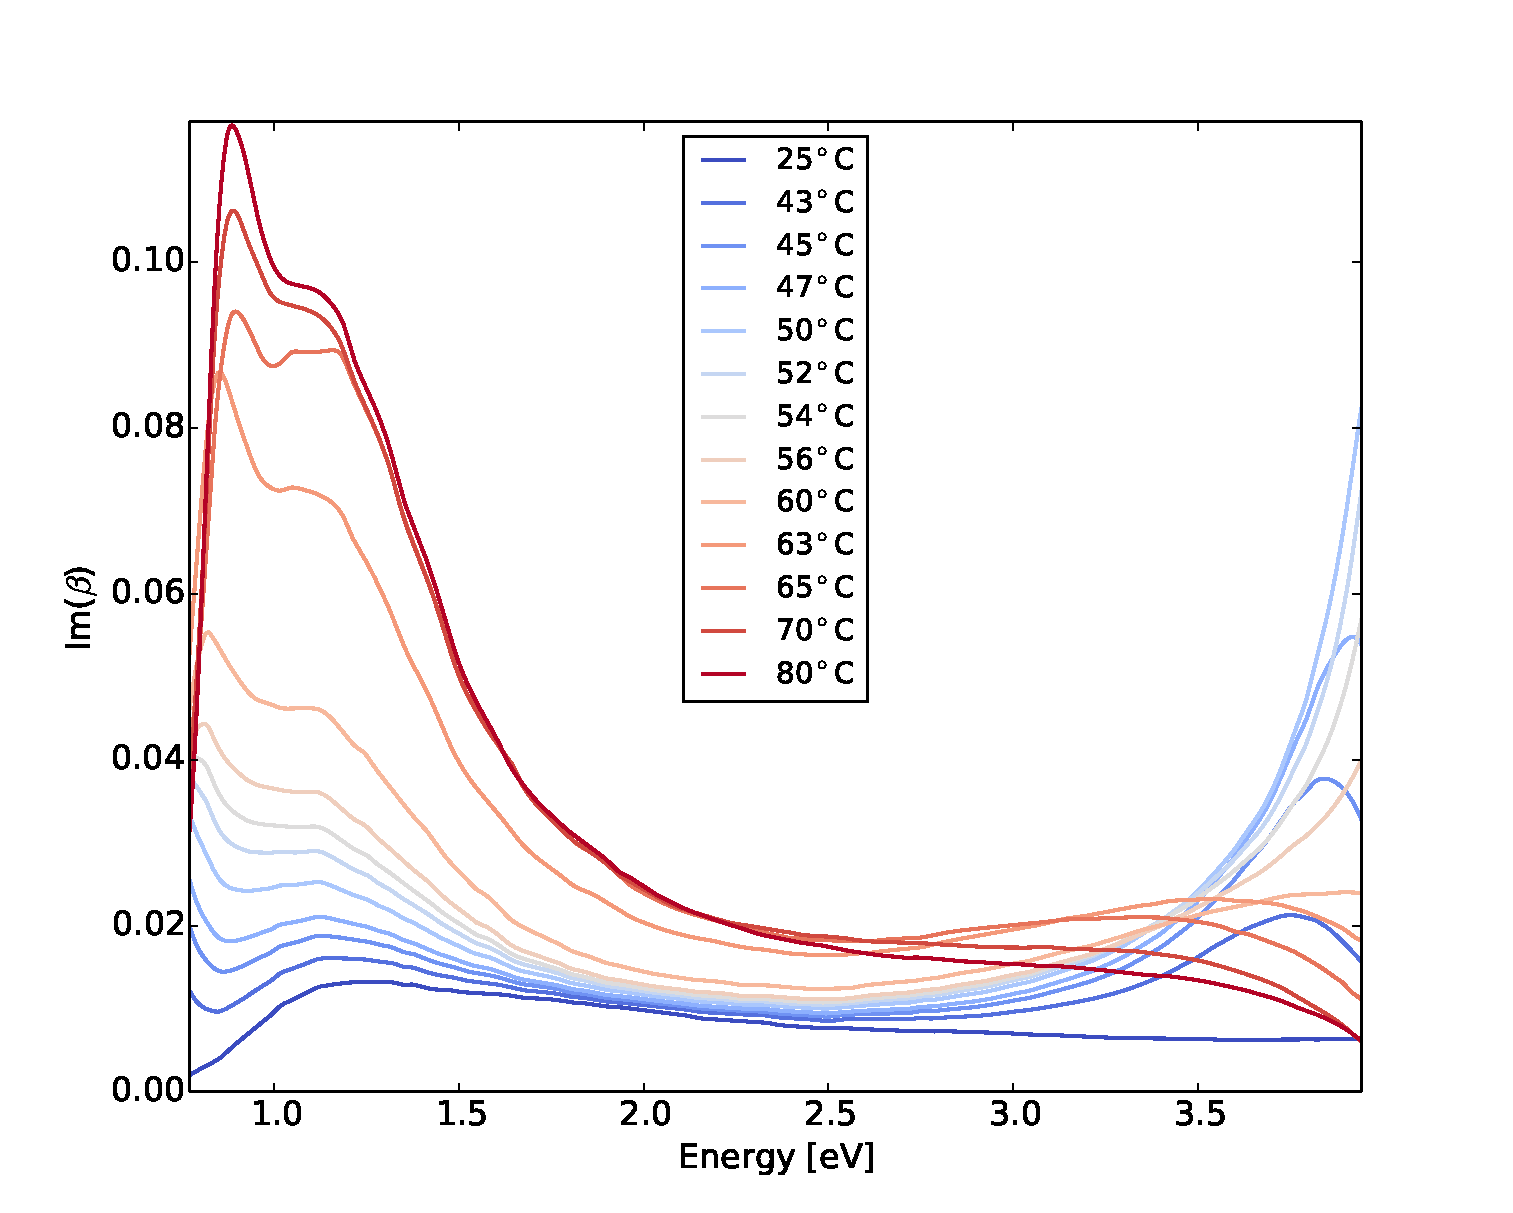
\includegraphics[width=\textwidth]{Results/Sim1/im_beta.pdf}
        \caption{}
        \label{fig:2}
    \end{subfigure}
    \caption{Relative reflectance $\Delta R/R$}
    \label{fig:}
\end{figure}
%


\section{Simulation 2; $R = 10$nm, s-polarized incident light}
\section{Simulation 3; $R = 15$nm, p-polarized incident light}
\section{Simulation 4; $R = 15$nm, s-polarized incident light}
\begin{figure}
    \centering
    \begin{subfigure}[b]{0.49\textwidth}
        \centering
        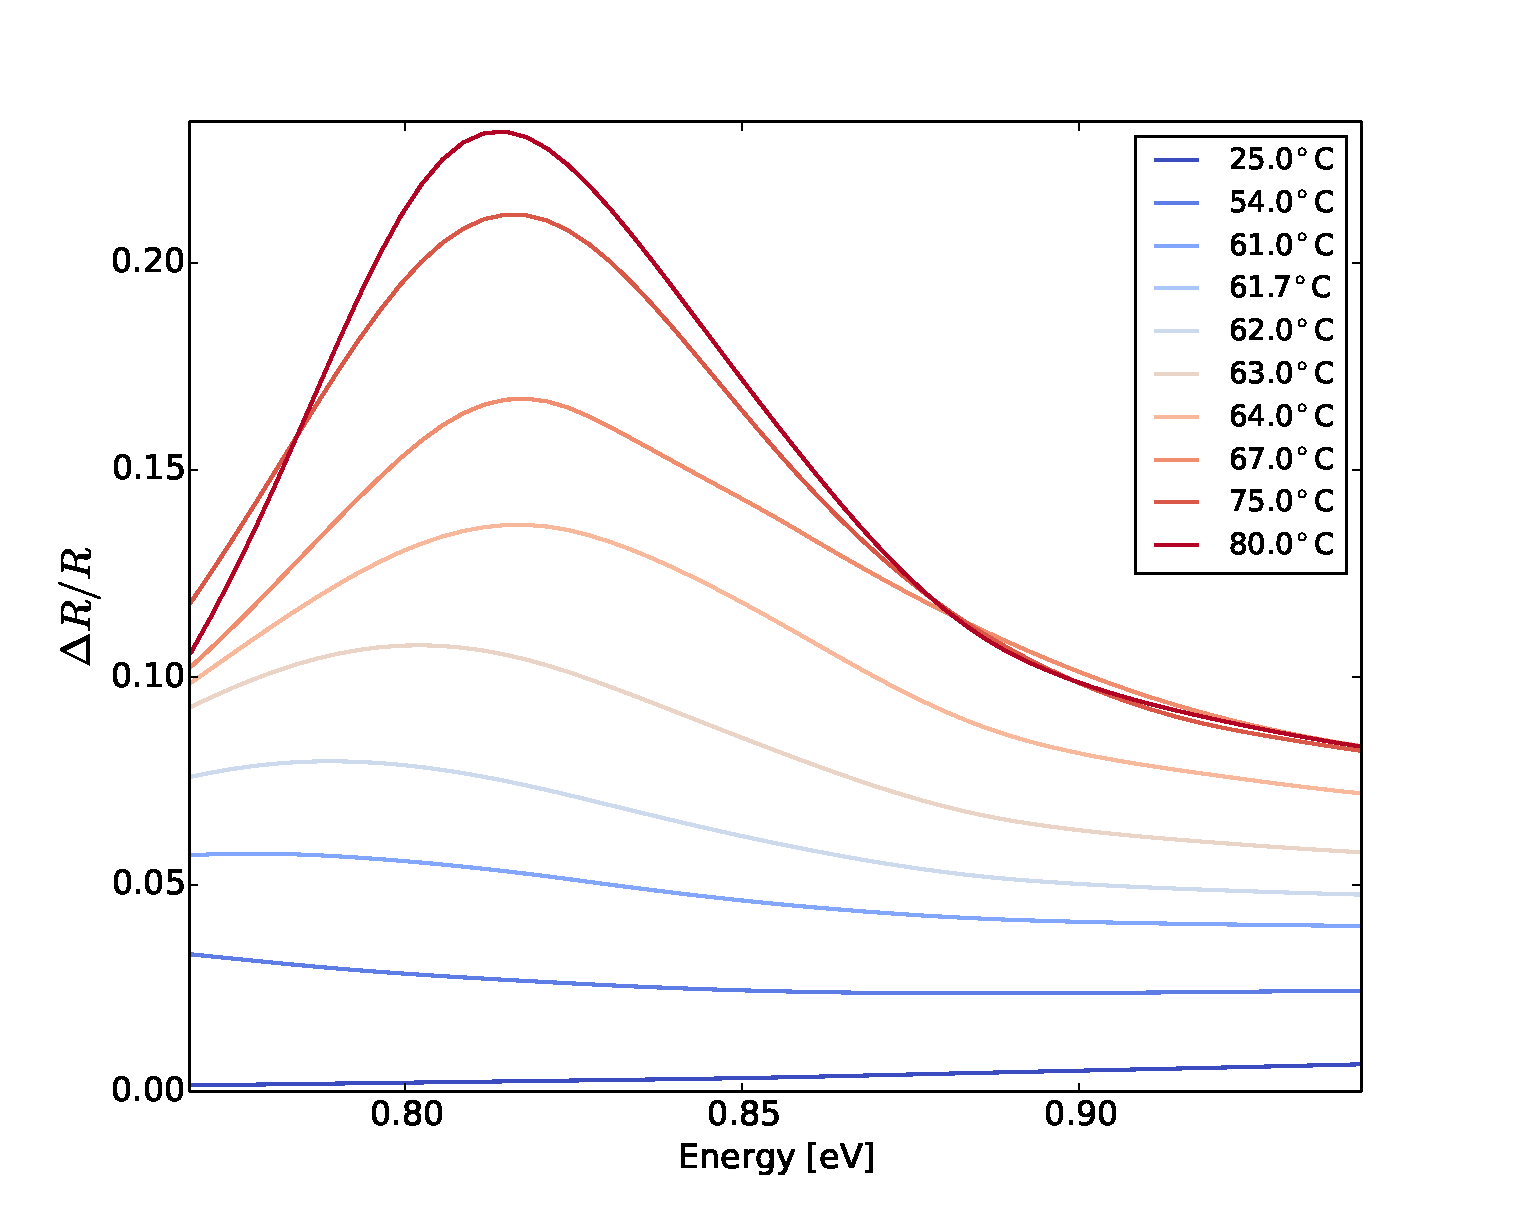
\includegraphics[width=\textwidth]{Results/Sim1/dR_lowE.pdf}
        \caption{$R=10$nm, p-polarization}
        \label{fig:y equals x}
    \end{subfigure}
    %\hfill
    \begin{subfigure}[b]{0.49\textwidth}
        \centering
        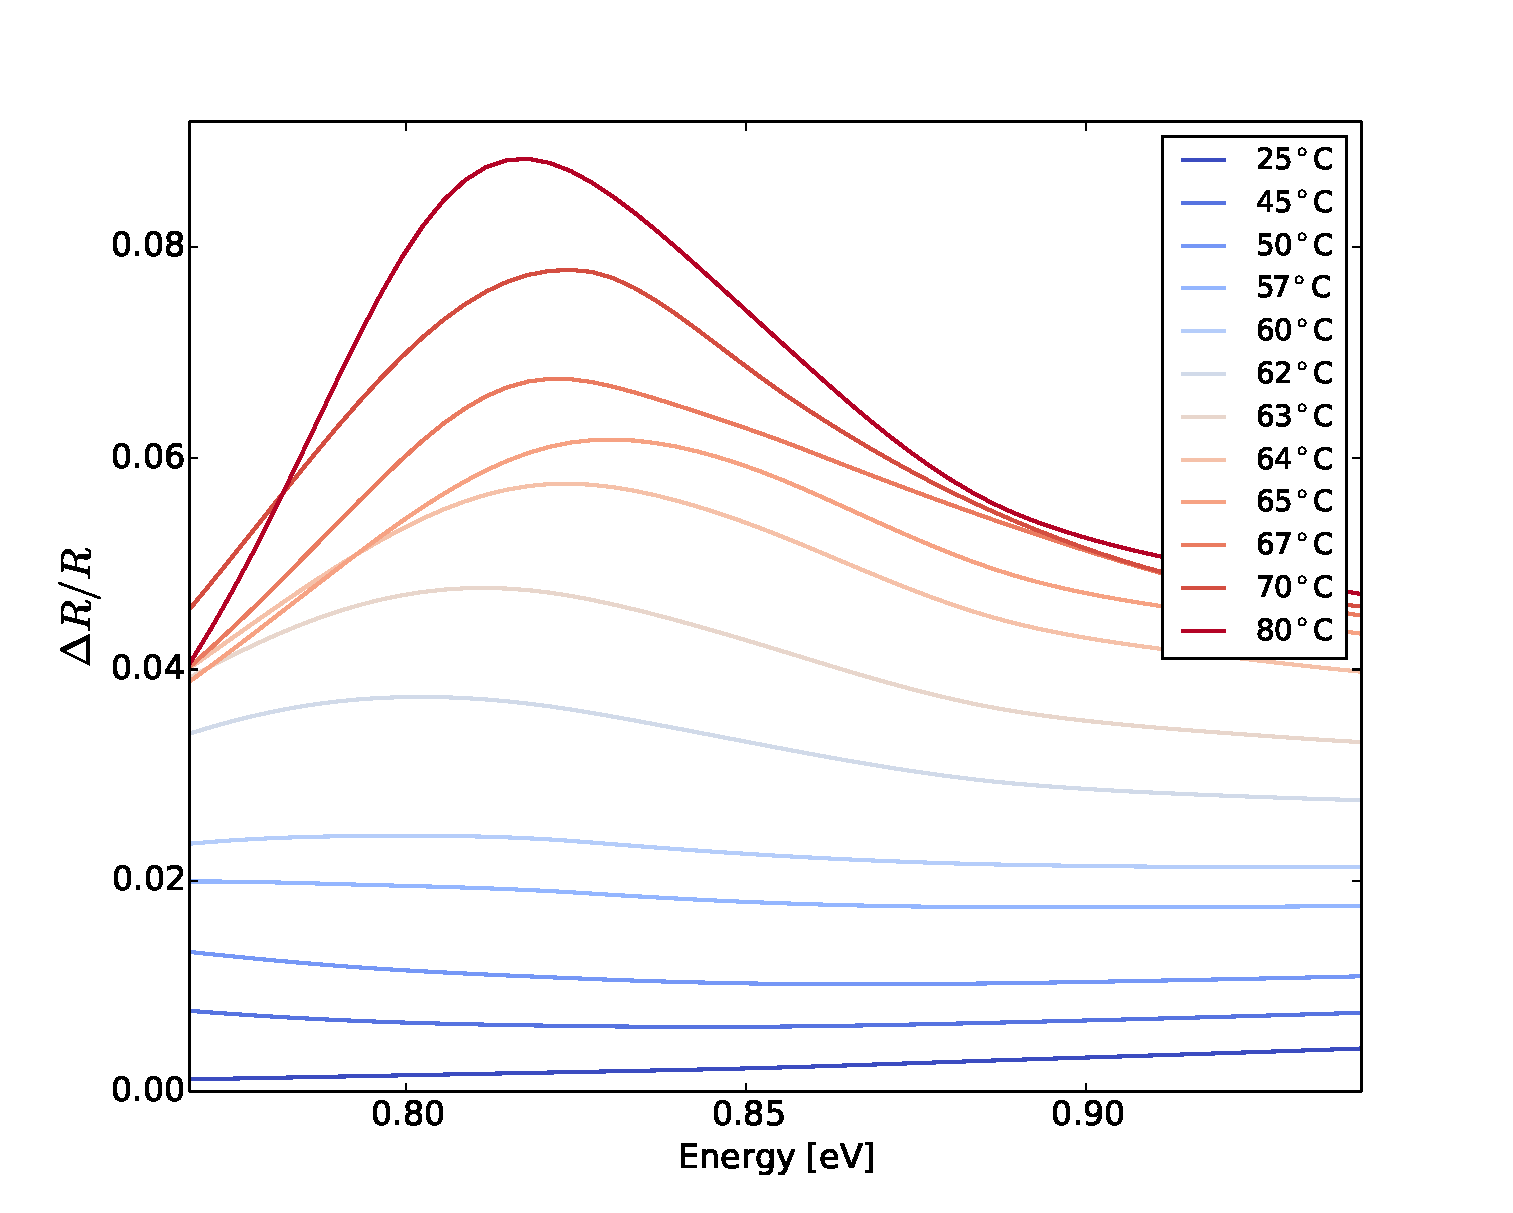
\includegraphics[width=\textwidth]{Results/Sim2/dR_lowE.pdf}
        \caption{$R=10$nm, s-polarization}
        \label{fig:five over x}
    \end{subfigure}
    %\hfill
    \begin{subfigure}[b]{0.49\textwidth}
        \centering
        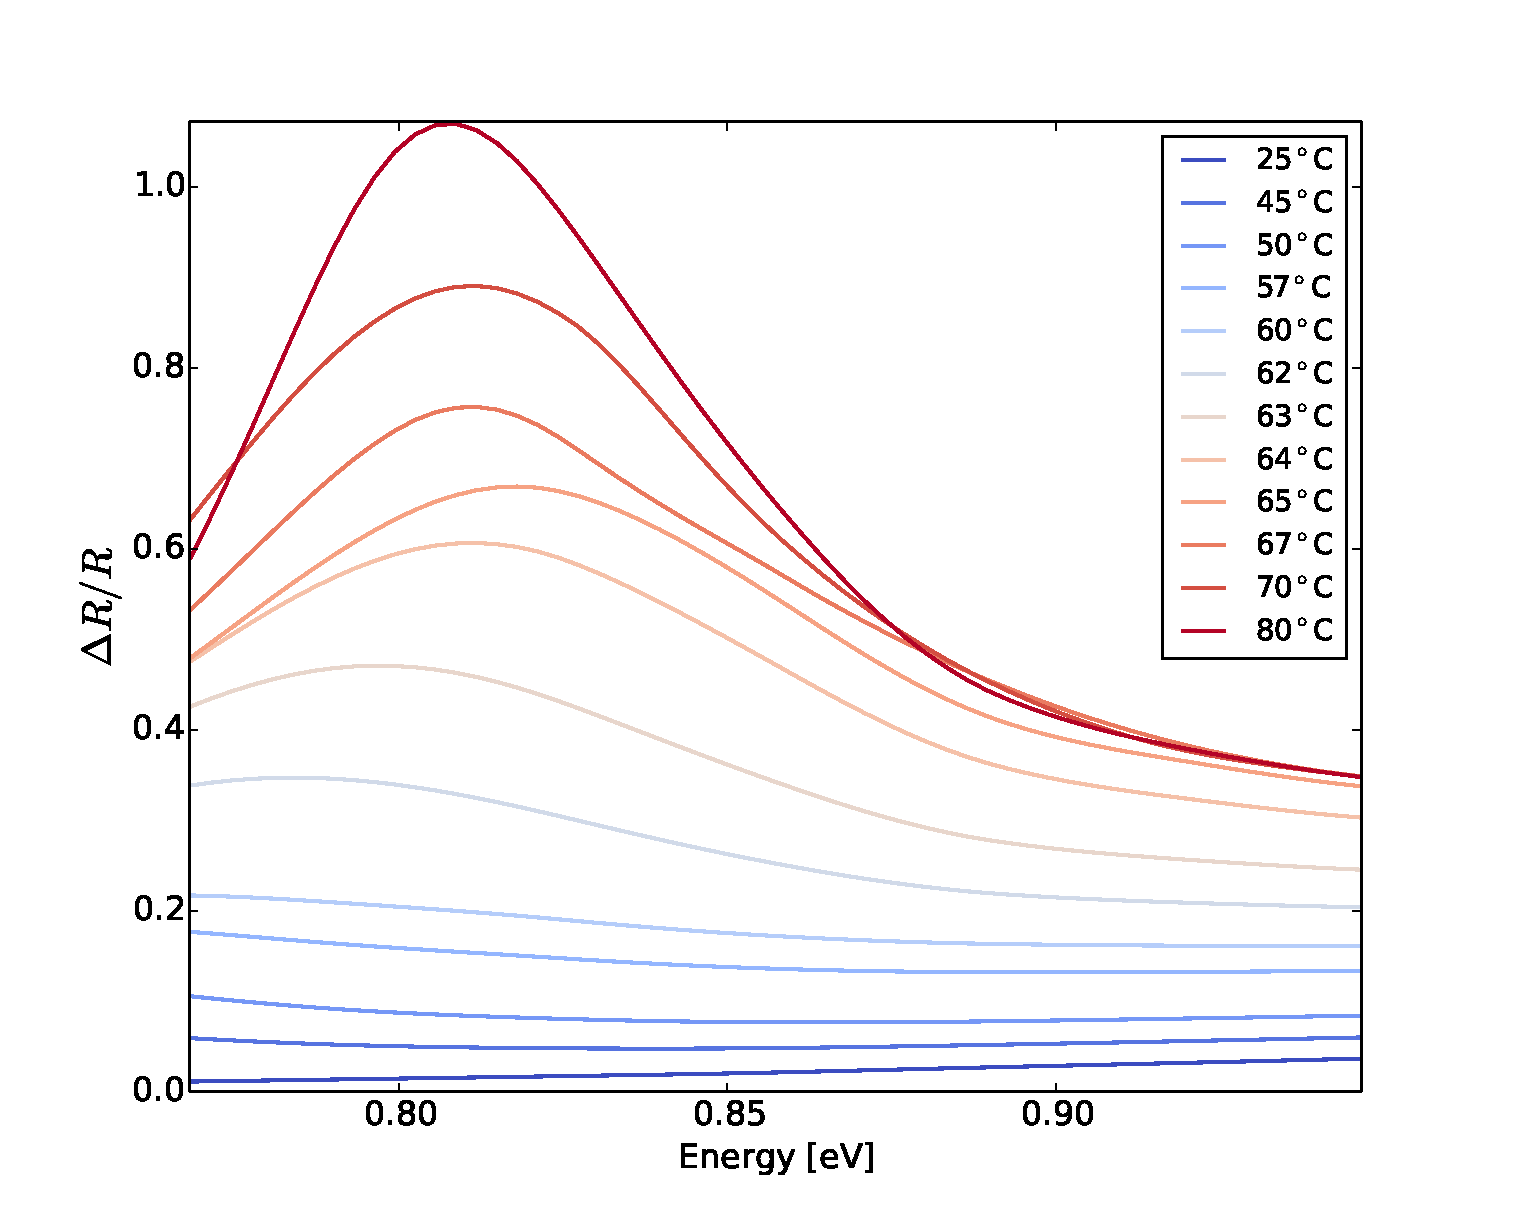
\includegraphics[width=\textwidth]{Results/Sim3/dR_lowE.pdf}
        \caption{$R=15$nm, p-polarization}
        \label{fig:three sin x}
    \end{subfigure}
    %\hfill
    \begin{subfigure}[b]{0.49\textwidth}
        \centering
        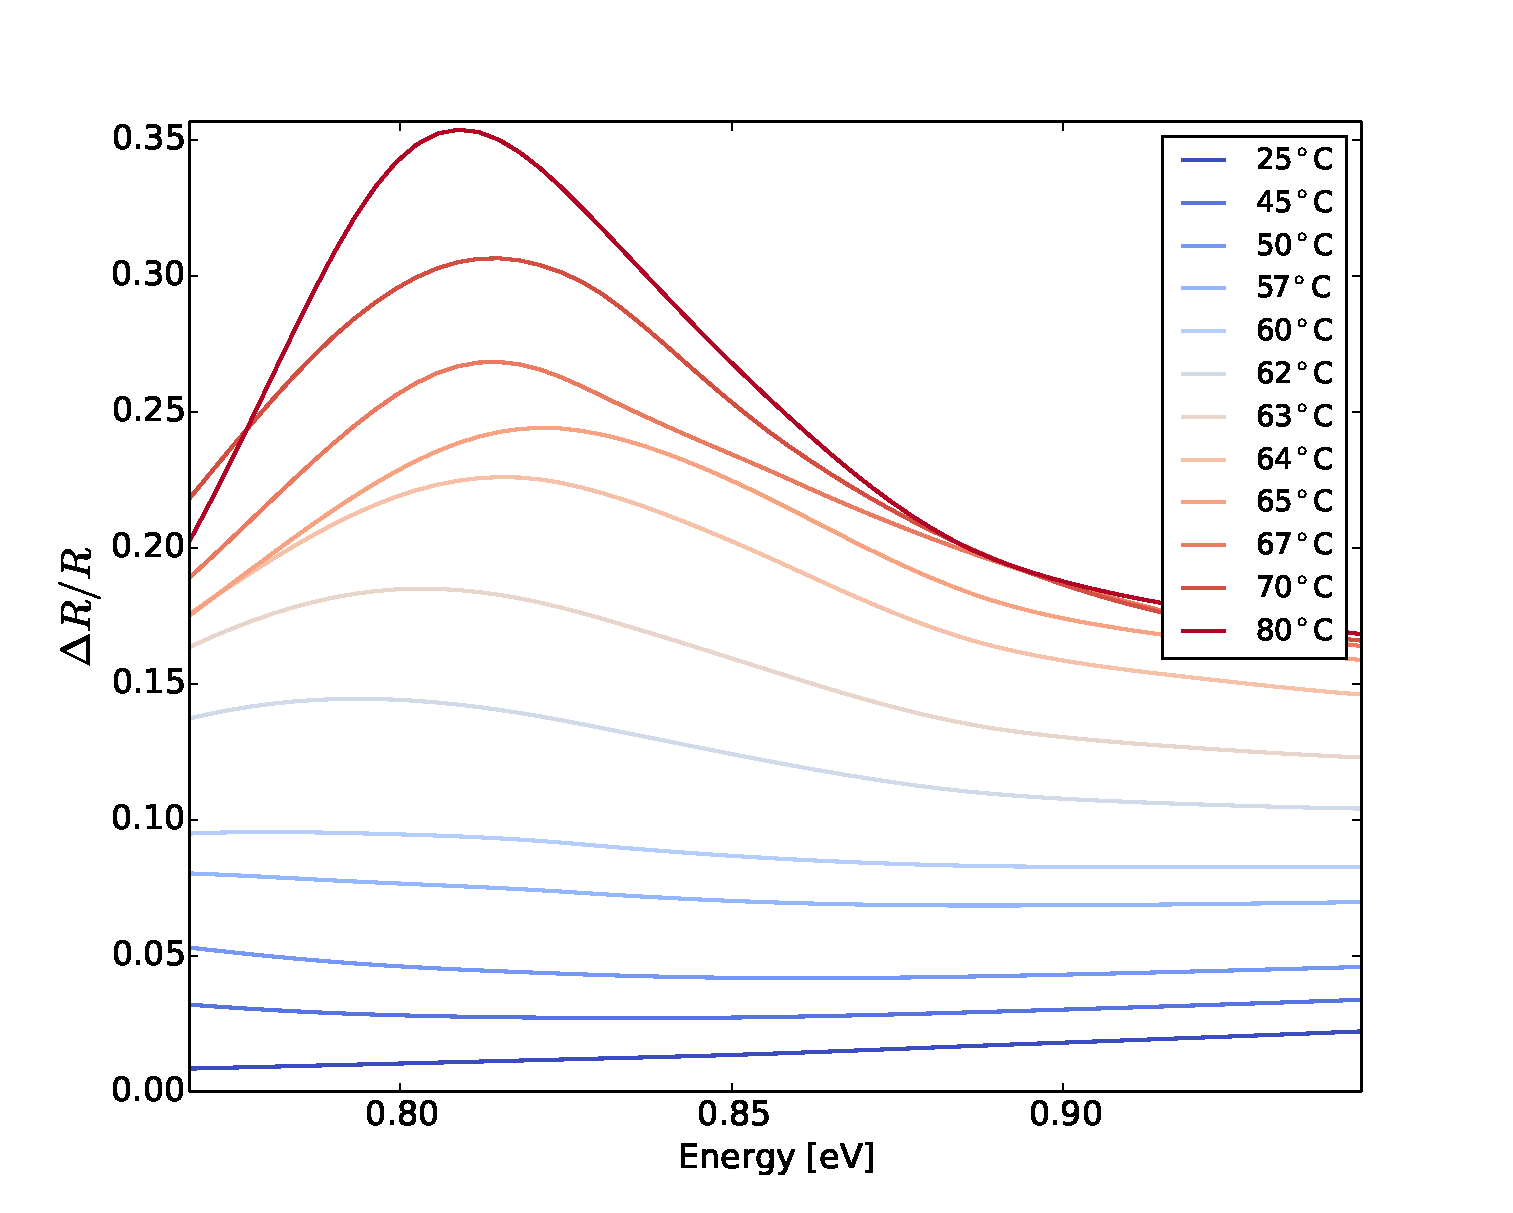
\includegraphics[width=\textwidth]{Results/Sim4/dR_lowE.pdf}
        \caption{$R=15$nm, s-polarization}
        \label{fig:five over x}
    \end{subfigure}
    \caption{Relative reflectance $\Delta R/R$}
    \label{fig:three graphs}
\end{figure}



\subsection{Color} \label{sec:color}
%
\begin{figure} [h!]
    \centering
    \begin{subfigure}[b]{0.49\textwidth}
        \centering
        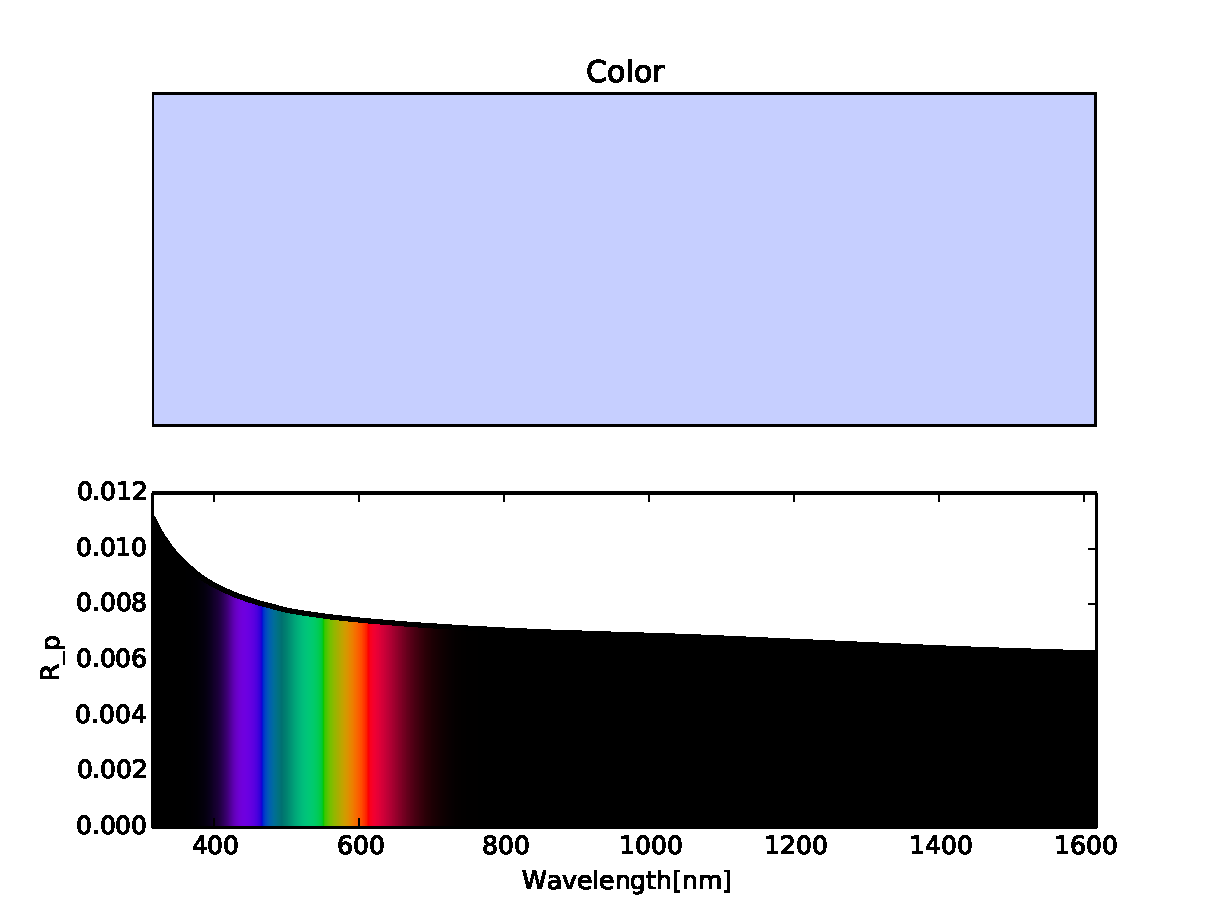
\includegraphics[width=\textwidth]{Results/Sim3/Rp_color25C.pdf}
        \caption{$T = 25^{\circ}$C}
        \label{fig:RpColor25C}
    \end{subfigure}
    %\hfill
    \begin{subfigure}[b]{0.49\textwidth}
        \centering
        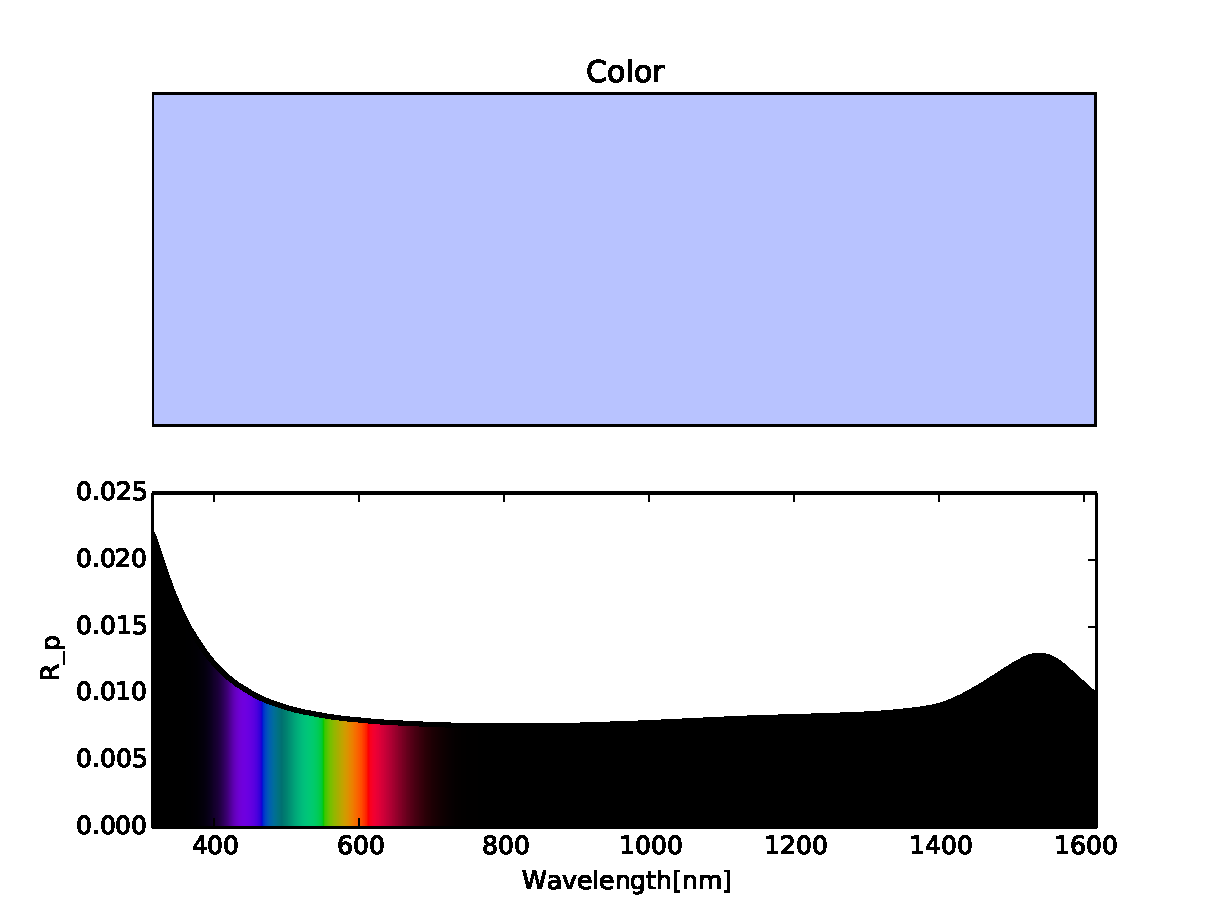
\includegraphics[width=\textwidth]{Results/Sim3/Rp_color80C.pdf}
        \caption{$T = 80^{\circ}$C}
        \label{fig:RpColor80C}
    \end{subfigure}
    \caption{
       The spectral reflectance for p-polarization together with the approximate resulting color.
       The simulation was done $r = 15$.
    }
    \label{fig:RpColor}
\end{figure}
%
%
\begin{figure}[h!]
    \centering
    \begin{subfigure}[b]{0.49\textwidth}
        \centering
        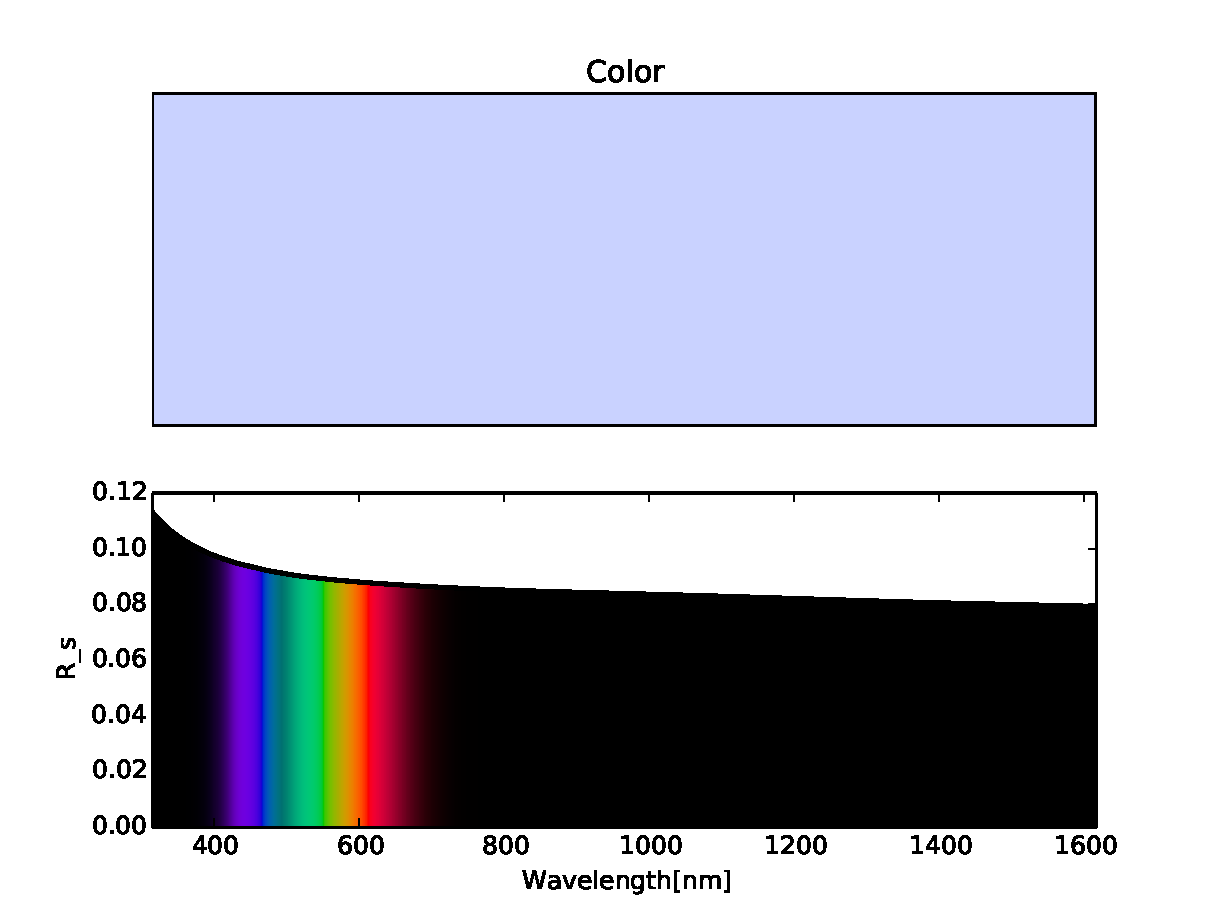
\includegraphics[width=\textwidth]{Results/Sim3/Rs_color25C.pdf}
        \caption{$T = 25^{\circ}$C}
        \label{fig:RsColor25C}
    \end{subfigure}
    %\hfill
    \begin{subfigure}[b]{0.49\textwidth}
        \centering
        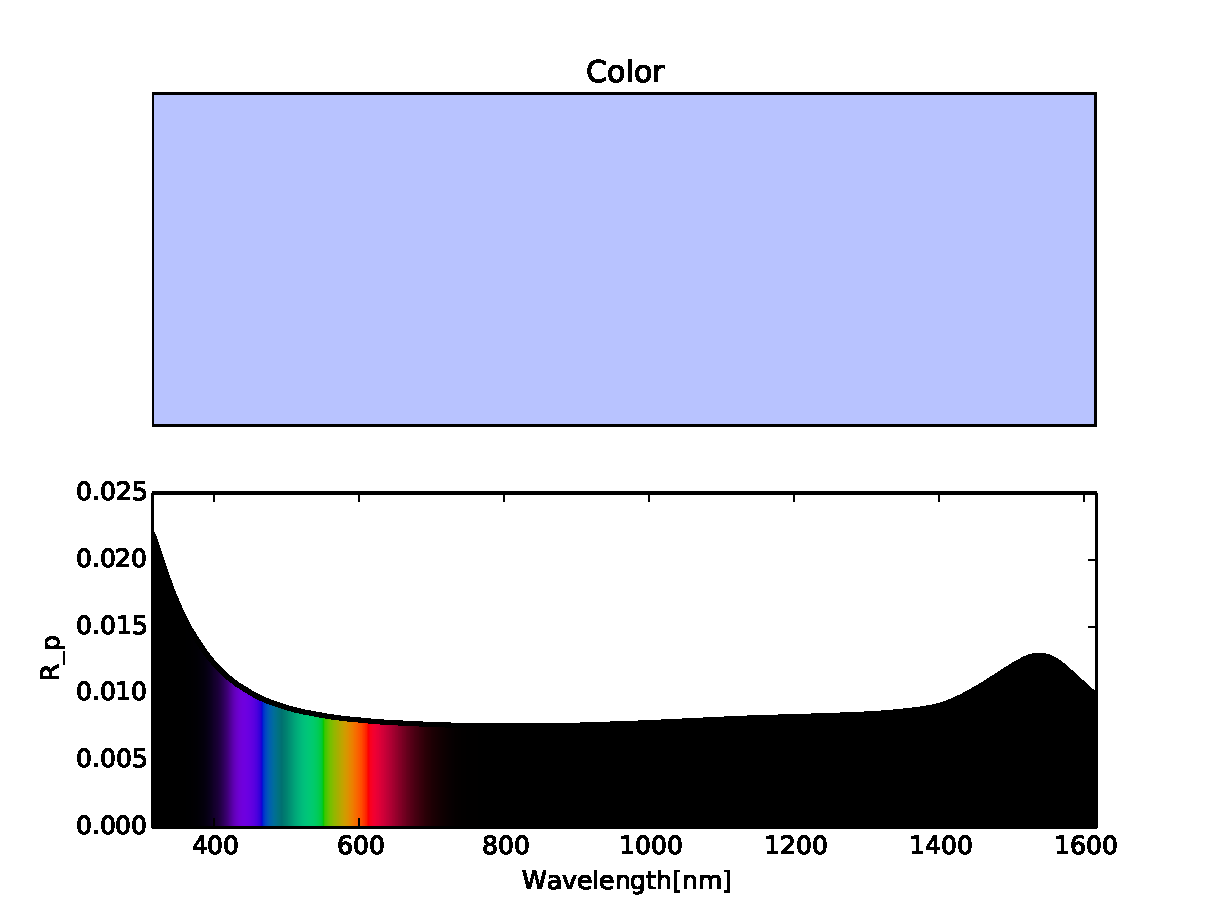
\includegraphics[width=\textwidth]{Results/Sim3/Rp_color80C.pdf}
        \caption{$T = 80^{\circ}$C}
        \label{fig:RsColor80C}
    \end{subfigure}
    \caption{
       The spectral reflectance for s-polarization together with the approximate resulting color.
       The simulation was done $r = 15$.
    }
    \label{fig:RsColor}
\end{figure}
%
%
\begin{figure}[h!]
    \centering
    \begin{subfigure}[b]{0.49\textwidth}
        \centering
        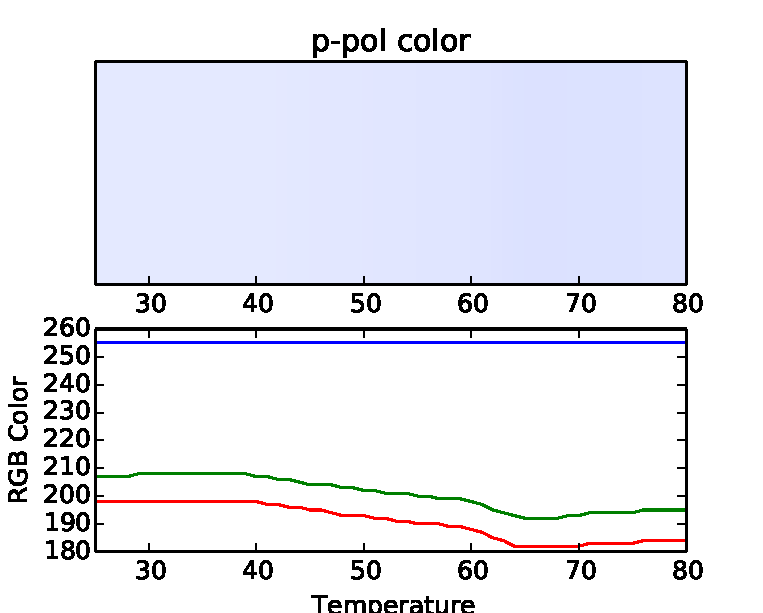
\includegraphics[width=\textwidth]{Results/Sim3/Rp_color.pdf}
        \caption{p-polarization}
        \label{fig:RpColor}
    \end{subfigure}
    %\hfill
    \begin{subfigure}[b]{0.49\textwidth}
        \centering
        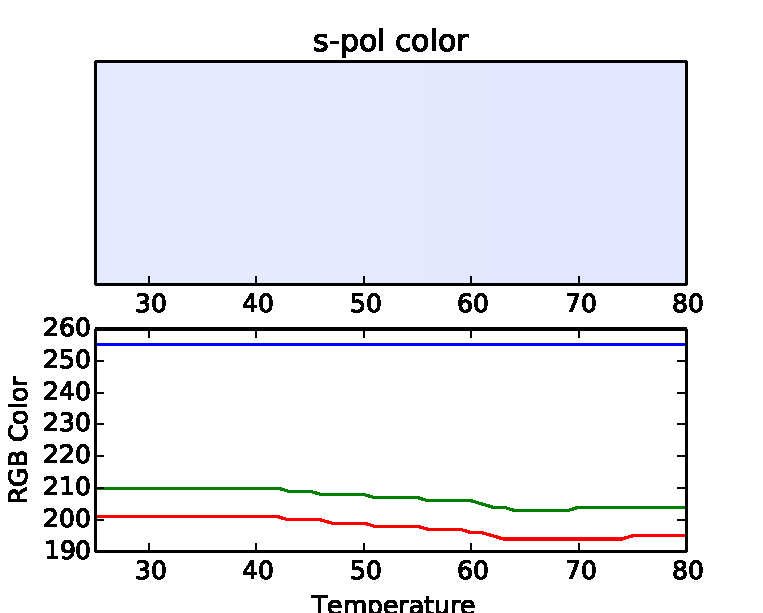
\includegraphics[width=\textwidth]{Results/Sim3/Rs_color.pdf}
        \caption{s-polarization}
        \label{fig:RsColor}
    \end{subfigure}
    \caption{
       The resulting approximated color together with the corresponding RGB values,
       based on the reflectance with $r = 15$ as a function of temperature.
    }
    \label{fig:RColor}
\end{figure}
%

%\section{Results}
\section{Interpolated Dielectric Function $\varepsilon(\omega,T)$}
%
\begin{figure}
    \centering
    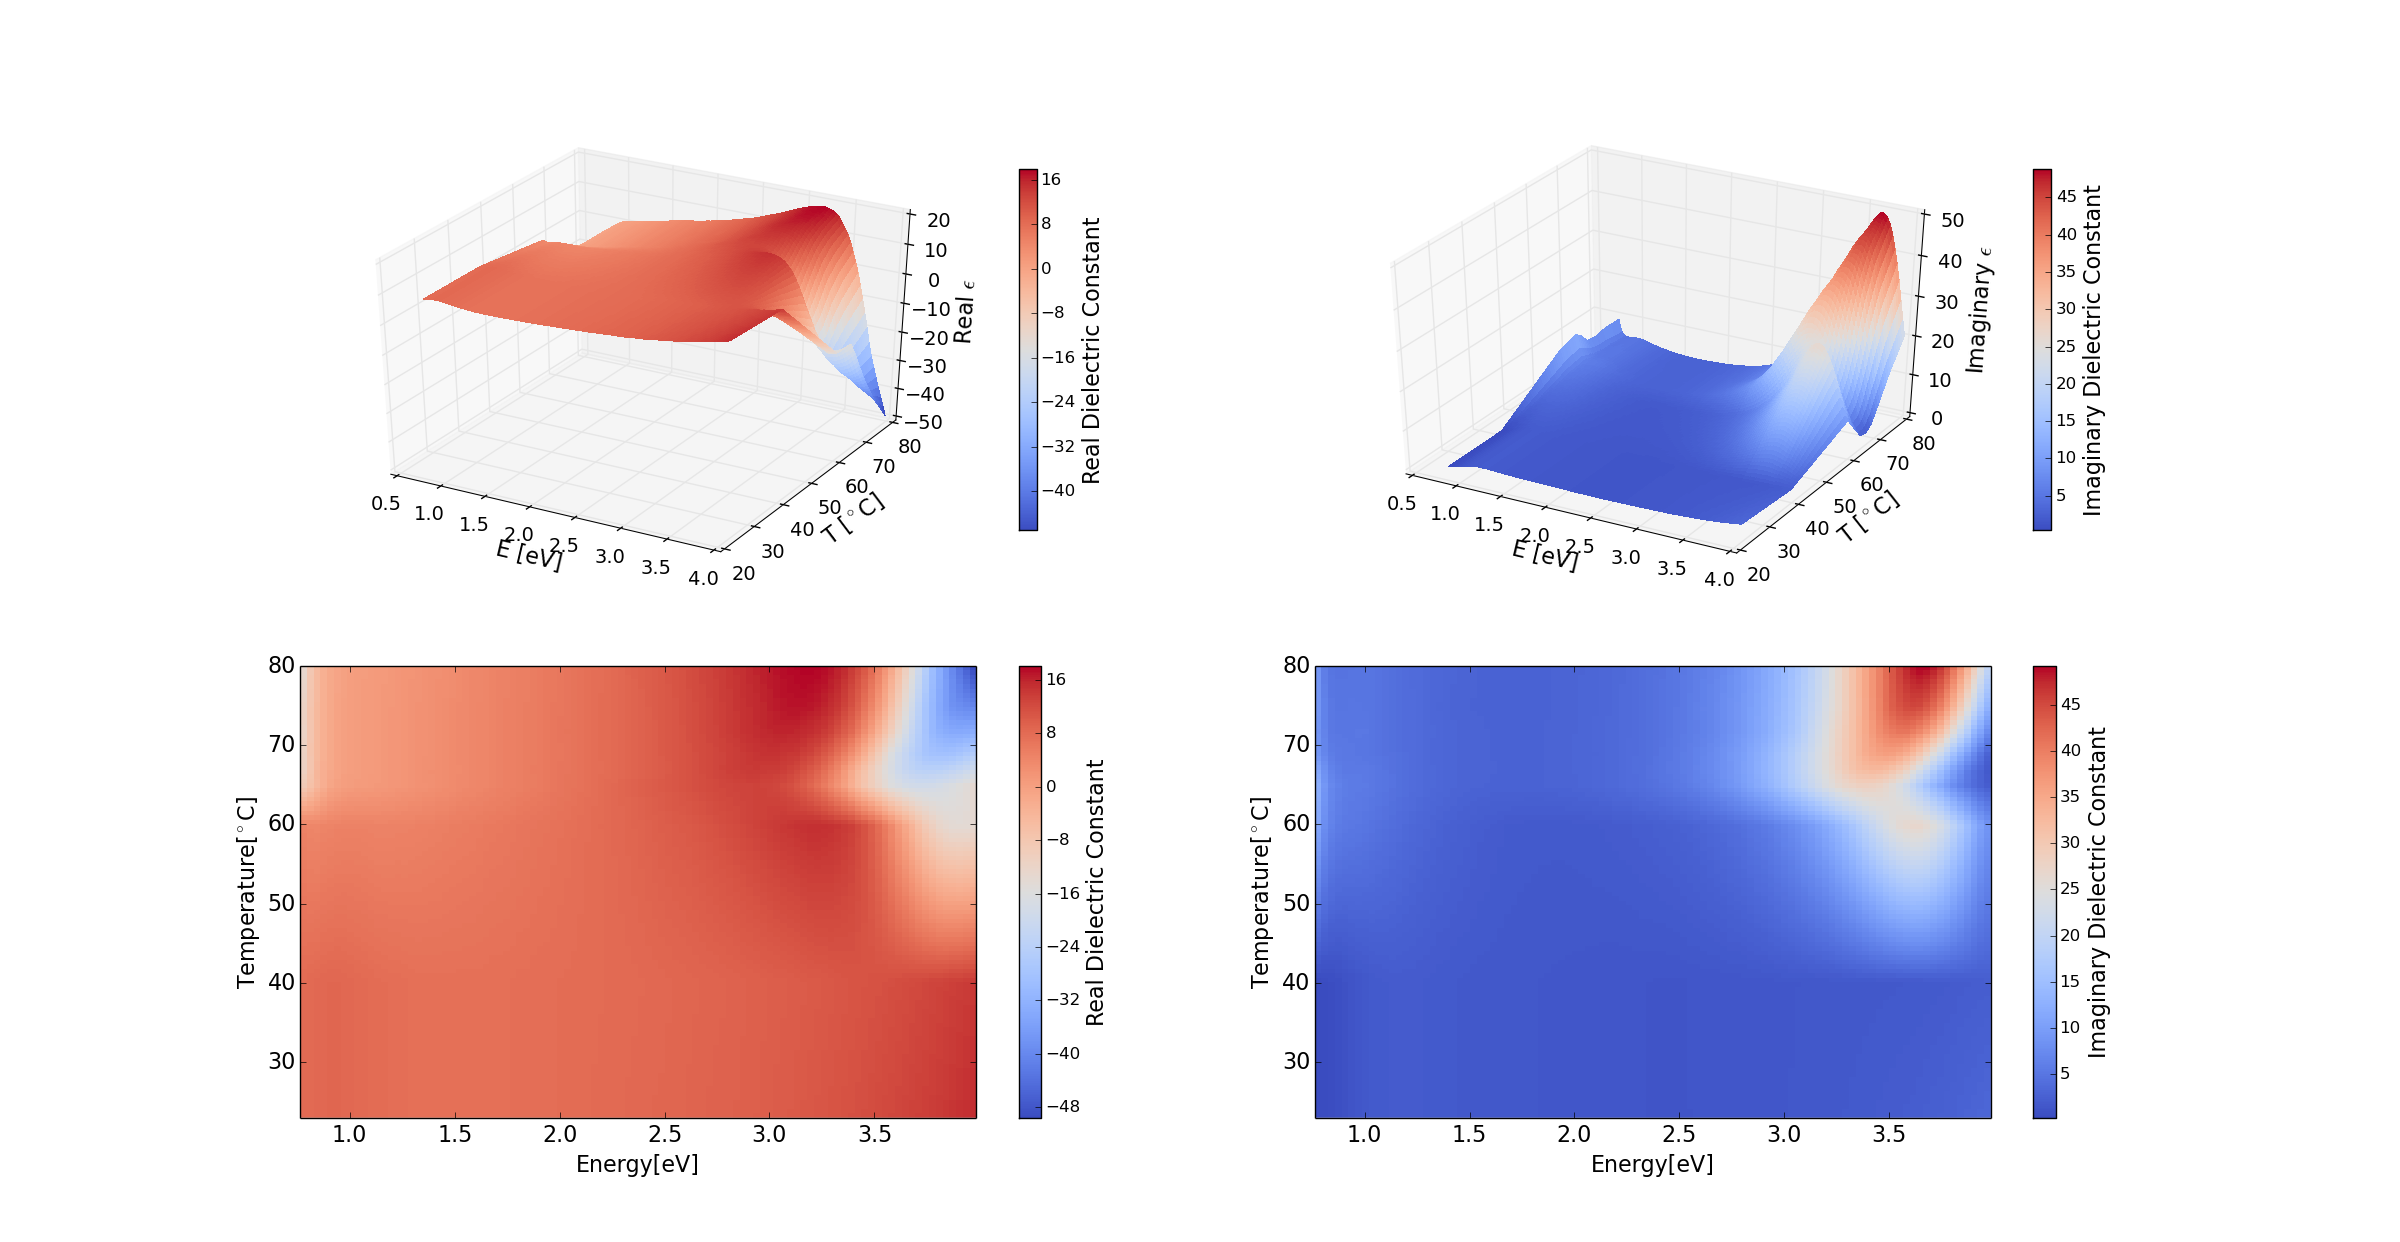
\includegraphics[width=\textwidth]{Results/interpPermittivity.png}
    \caption{Dielectric Function}
    \label{fig:DF}
\end{figure}
%

\section{Simulation results}
The following simulations are done with an incident plane wave of direction 
$(\theta_i,\phi_i) = (45^{\circ},0^{\circ})$, on VO$_2$ particles supported by a SiO$_2$ substrate
with truncation ratio $t_r = 0$. The surrounding medium is air with $\varepsilon(\omega,T) = 1$.
The particles are arranged in a square lattice with lattice constant $L = 45$nm and the
particle-particle interaction is given by a dipole contribution. The multipole truncation
is set to $M = 16$.


\subsection{Simulation 1; $R = 10$nm, p-polarized incident light}
%
\begin{figure}
    \centering
    \begin{subfigure}[b]{0.49\textwidth}
        \centering
        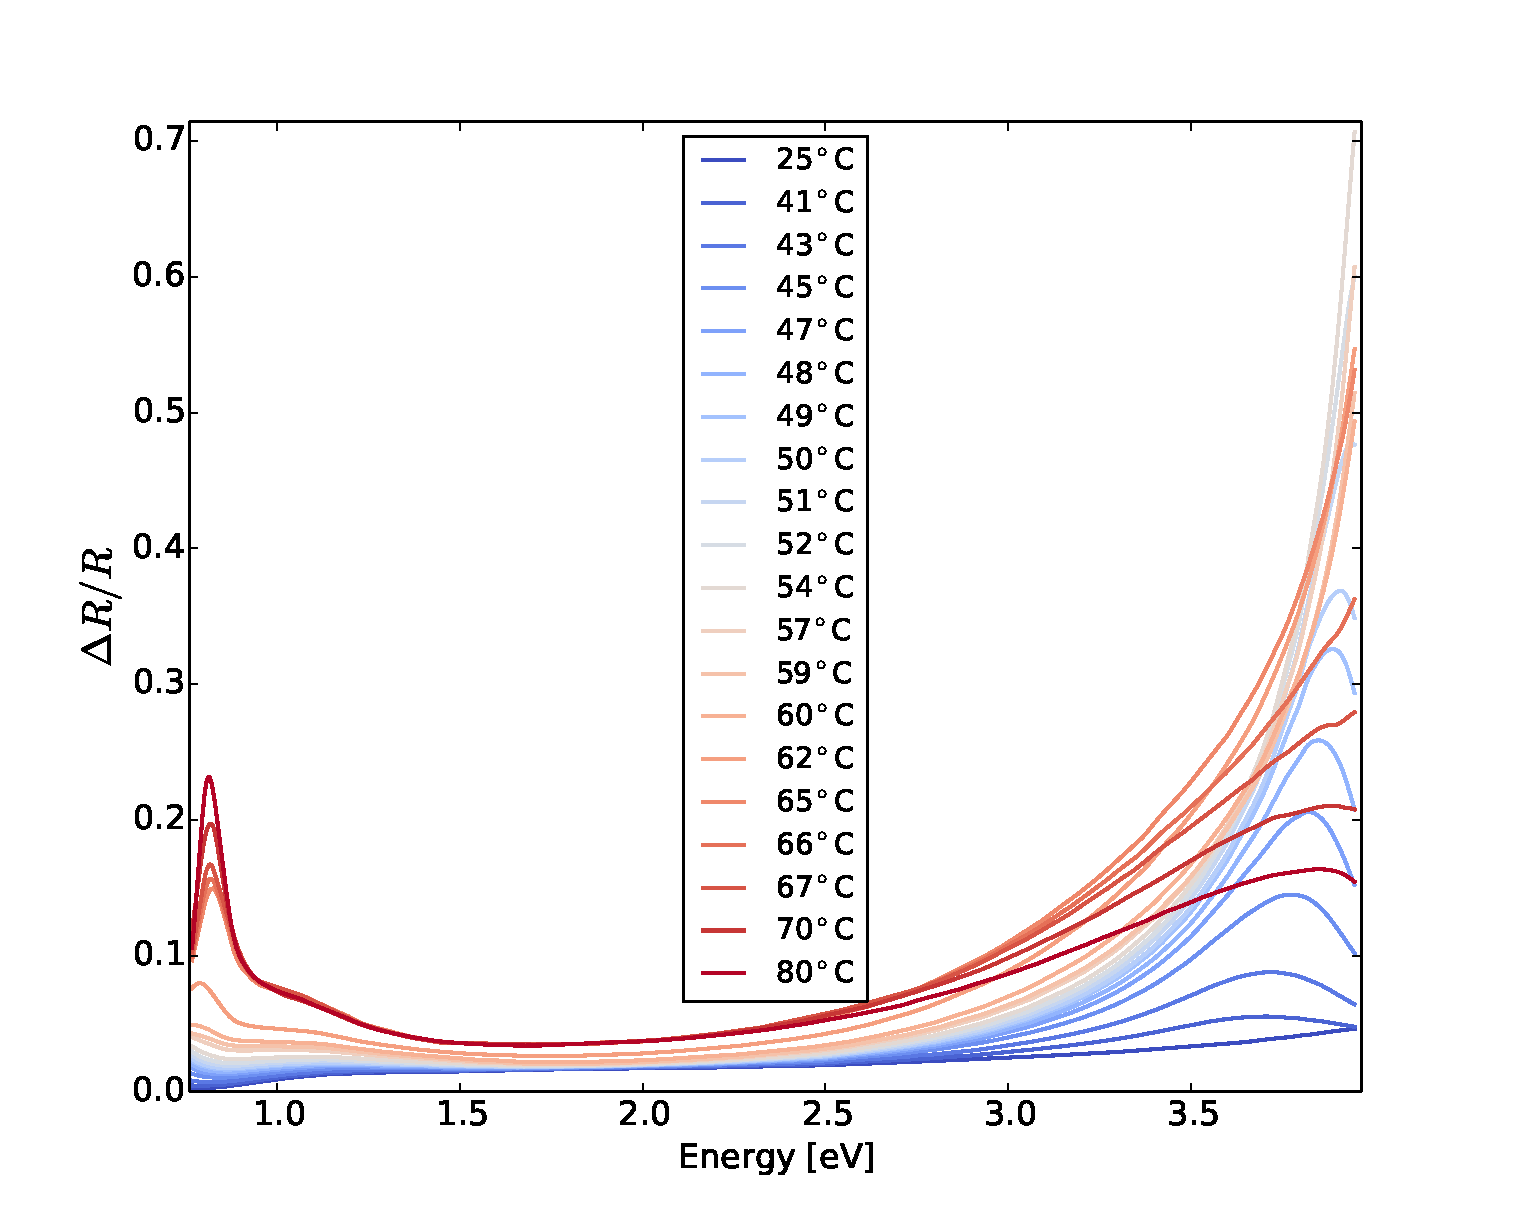
\includegraphics[width=\textwidth]{Results/Sim1/dR.pdf}
        \caption{}
        \label{fig:}
    \end{subfigure}
    %\hfill
    \begin{subfigure}[b]{0.49\textwidth}
        \centering
        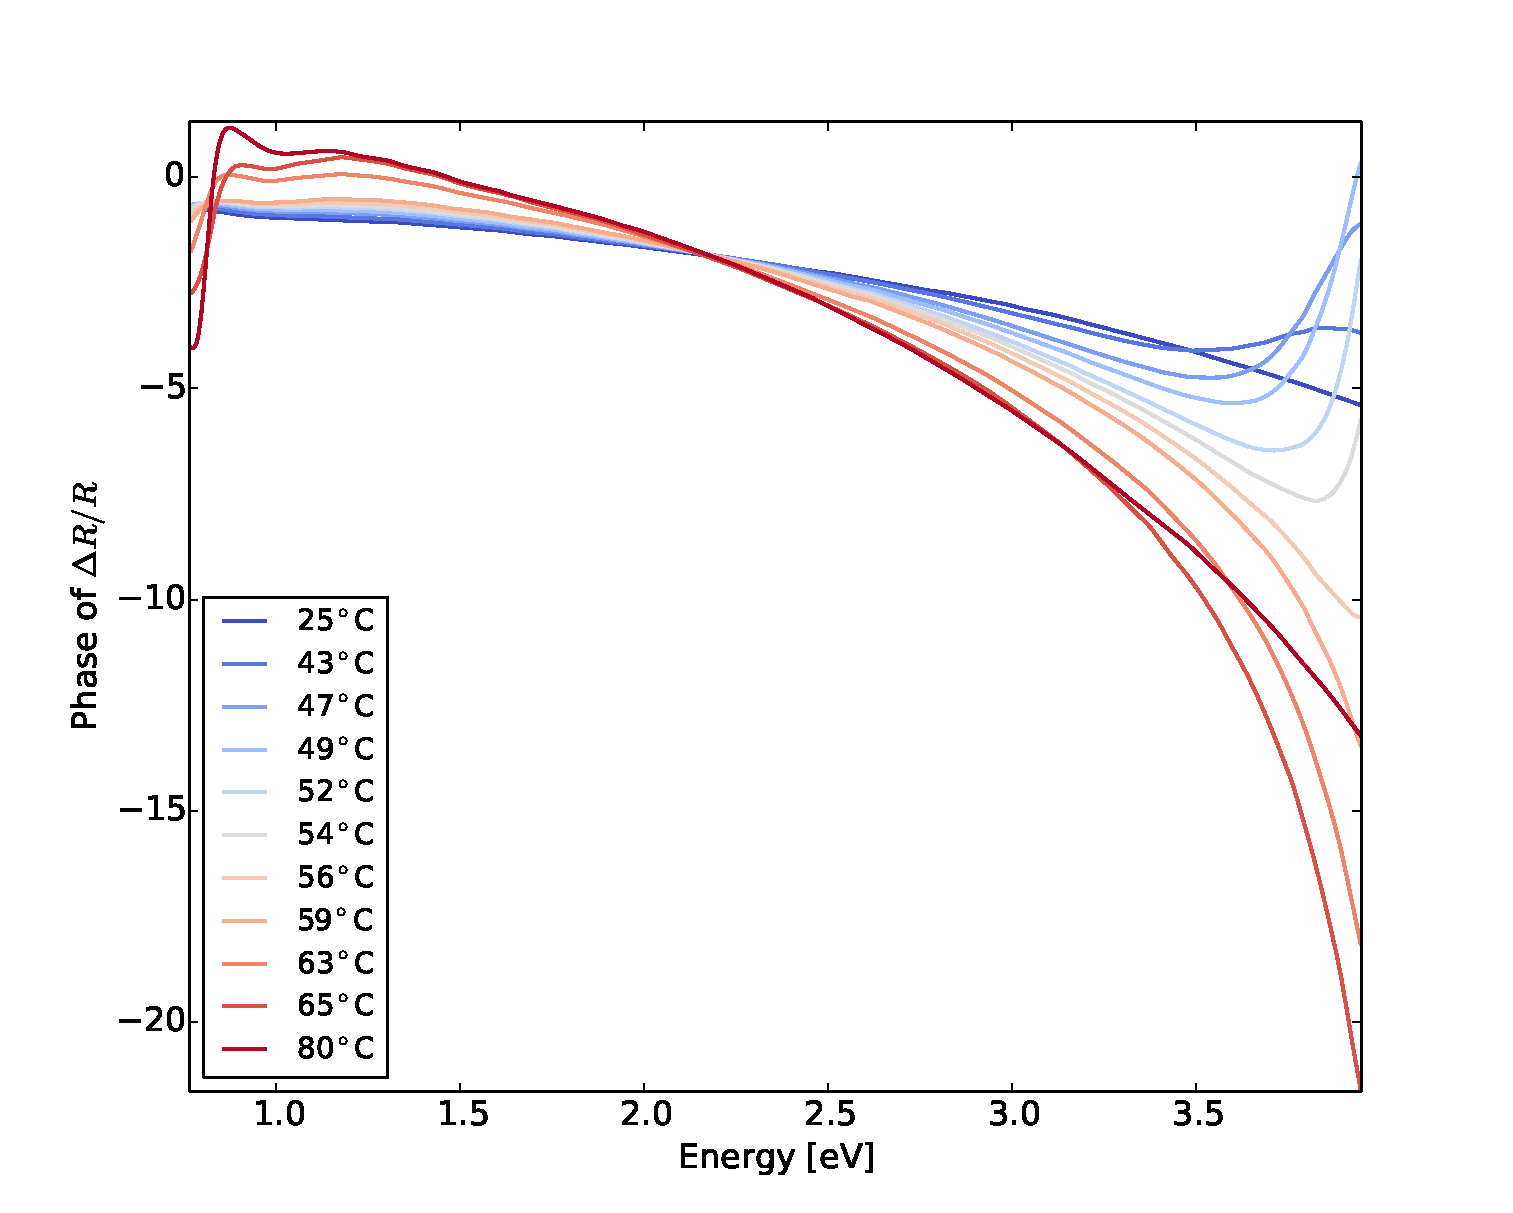
\includegraphics[width=\textwidth]{Results/Sim1/dRphase.pdf}
        \caption{}
        \label{fig:}
    \end{subfigure}
    \caption{Relative reflectance $\Delta R/R$}
    \label{fig:1}
\end{figure}
%
%
\begin{figure}
    \centering
    \begin{subfigure}[b]{0.49\textwidth}
        \centering
        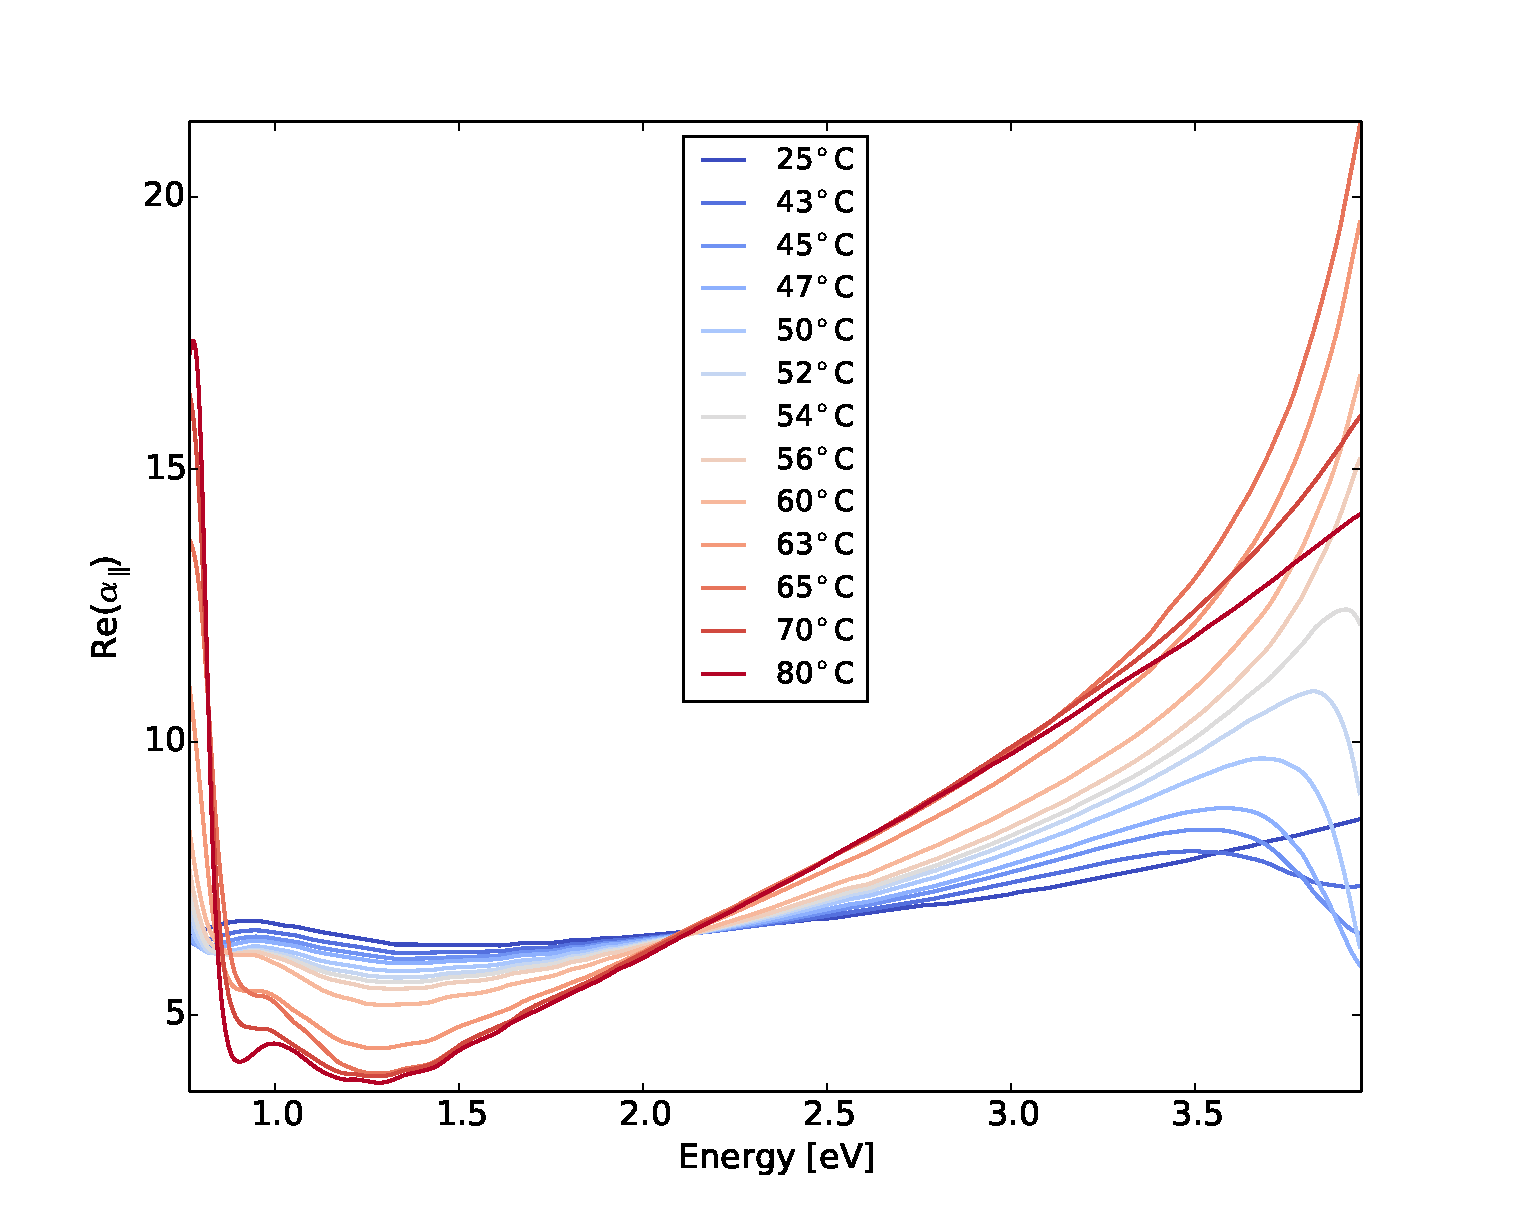
\includegraphics[width=\textwidth]{Results/Sim1/re_alpha_parallel.pdf}
        \caption{}
        \label{fig:2}
    \end{subfigure}
    %\hfill
    \begin{subfigure}[b]{0.49\textwidth}
        \centering
        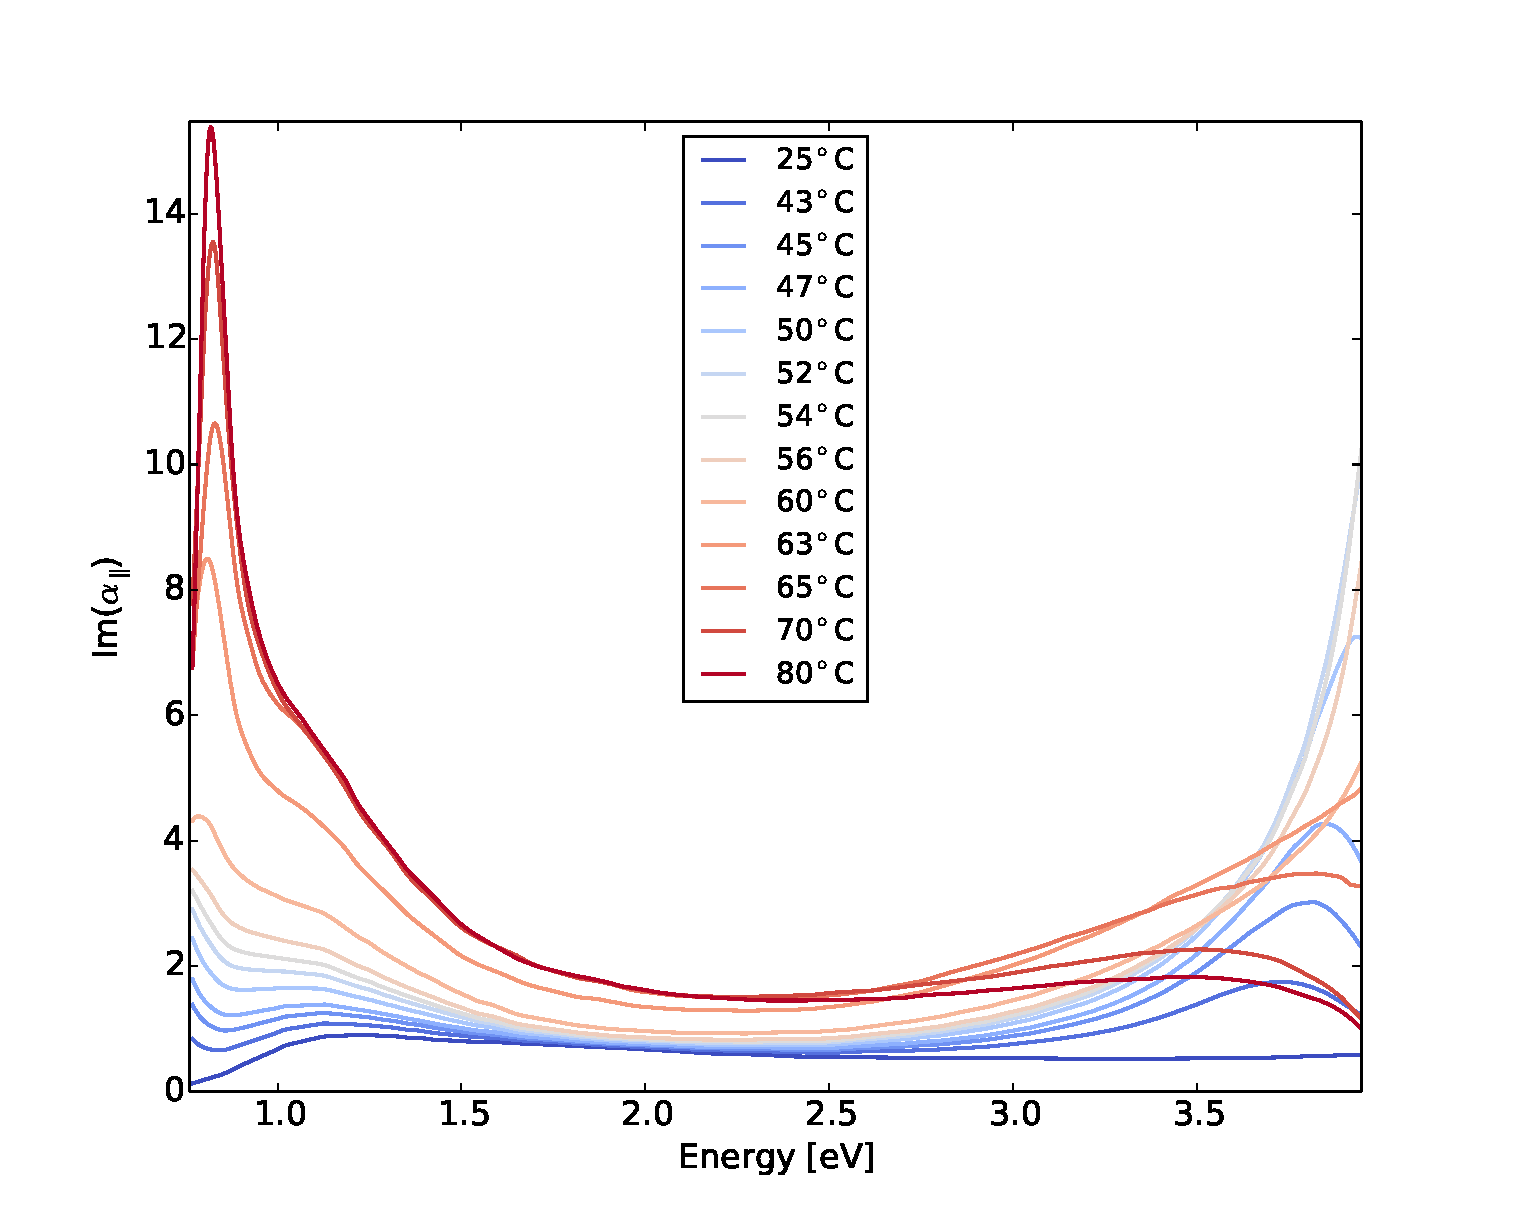
\includegraphics[width=\textwidth]{Results/Sim1/im_alpha_parallel.pdf}
        \caption{}
        \label{fig:2}
    \end{subfigure}
    %\hfill
    \begin{subfigure}[b]{0.49\textwidth}
        \centering
        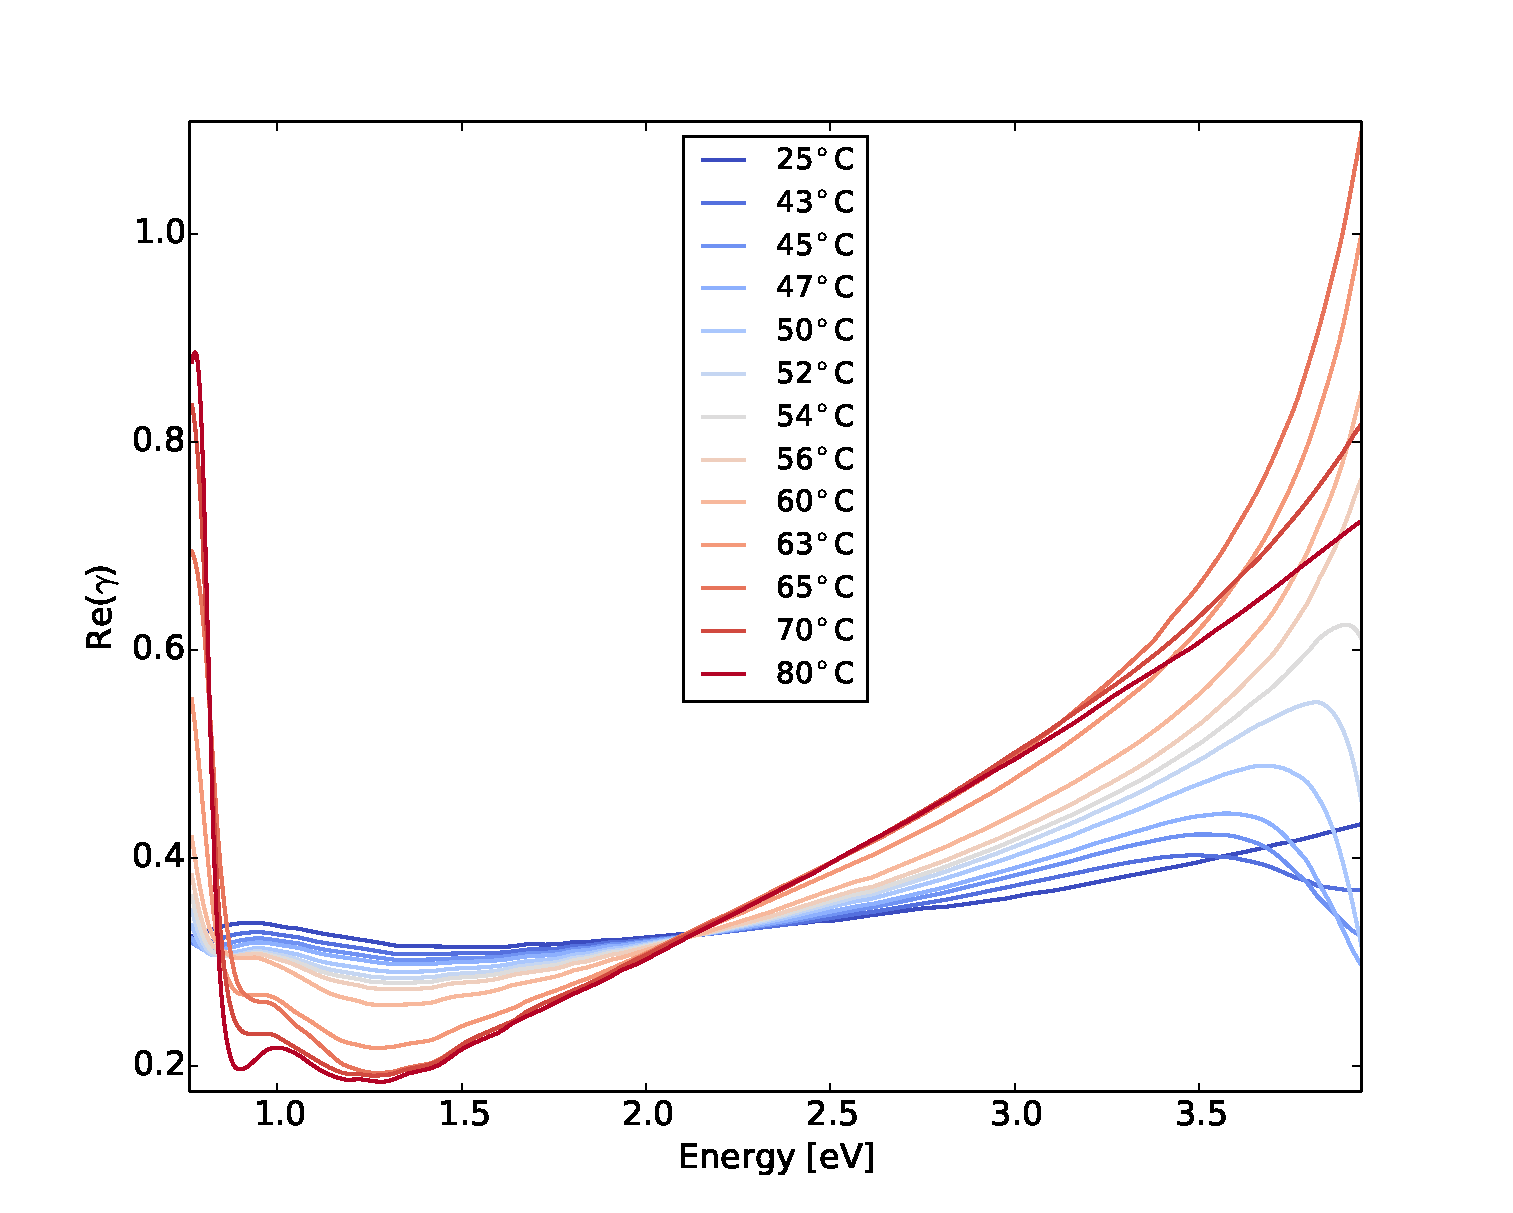
\includegraphics[width=\textwidth]{Results/Sim1/re_gamma.pdf}
        \caption{}
        \label{fig:2}
    \end{subfigure}
    %\hfill
    \begin{subfigure}[b]{0.49\textwidth}
        \centering
        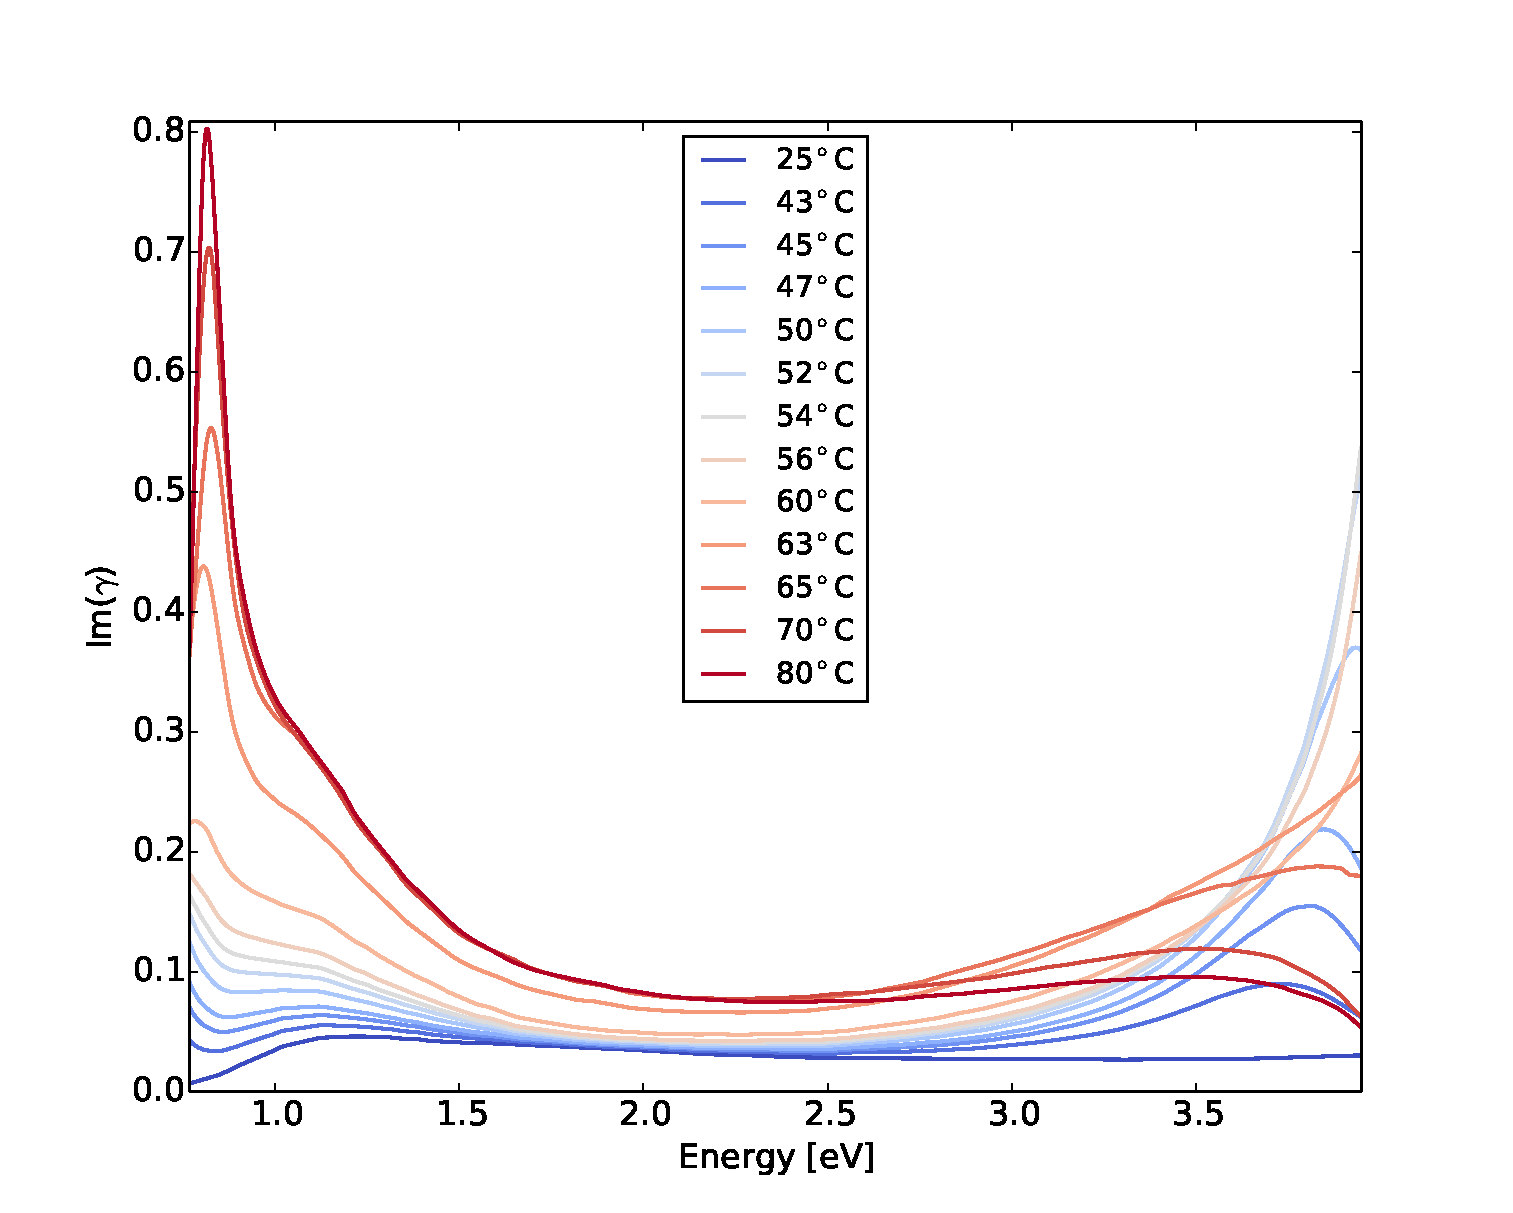
\includegraphics[width=\textwidth]{Results/Sim1/im_gamma.pdf}
        \caption{}
        \label{fig:2}
    \end{subfigure}
    \caption{Relative reflectance $\Delta R/R$}
    \label{fig:}
\end{figure}
%
%
\begin{figure}
    \centering
    \begin{subfigure}[b]{0.49\textwidth}
        \centering
        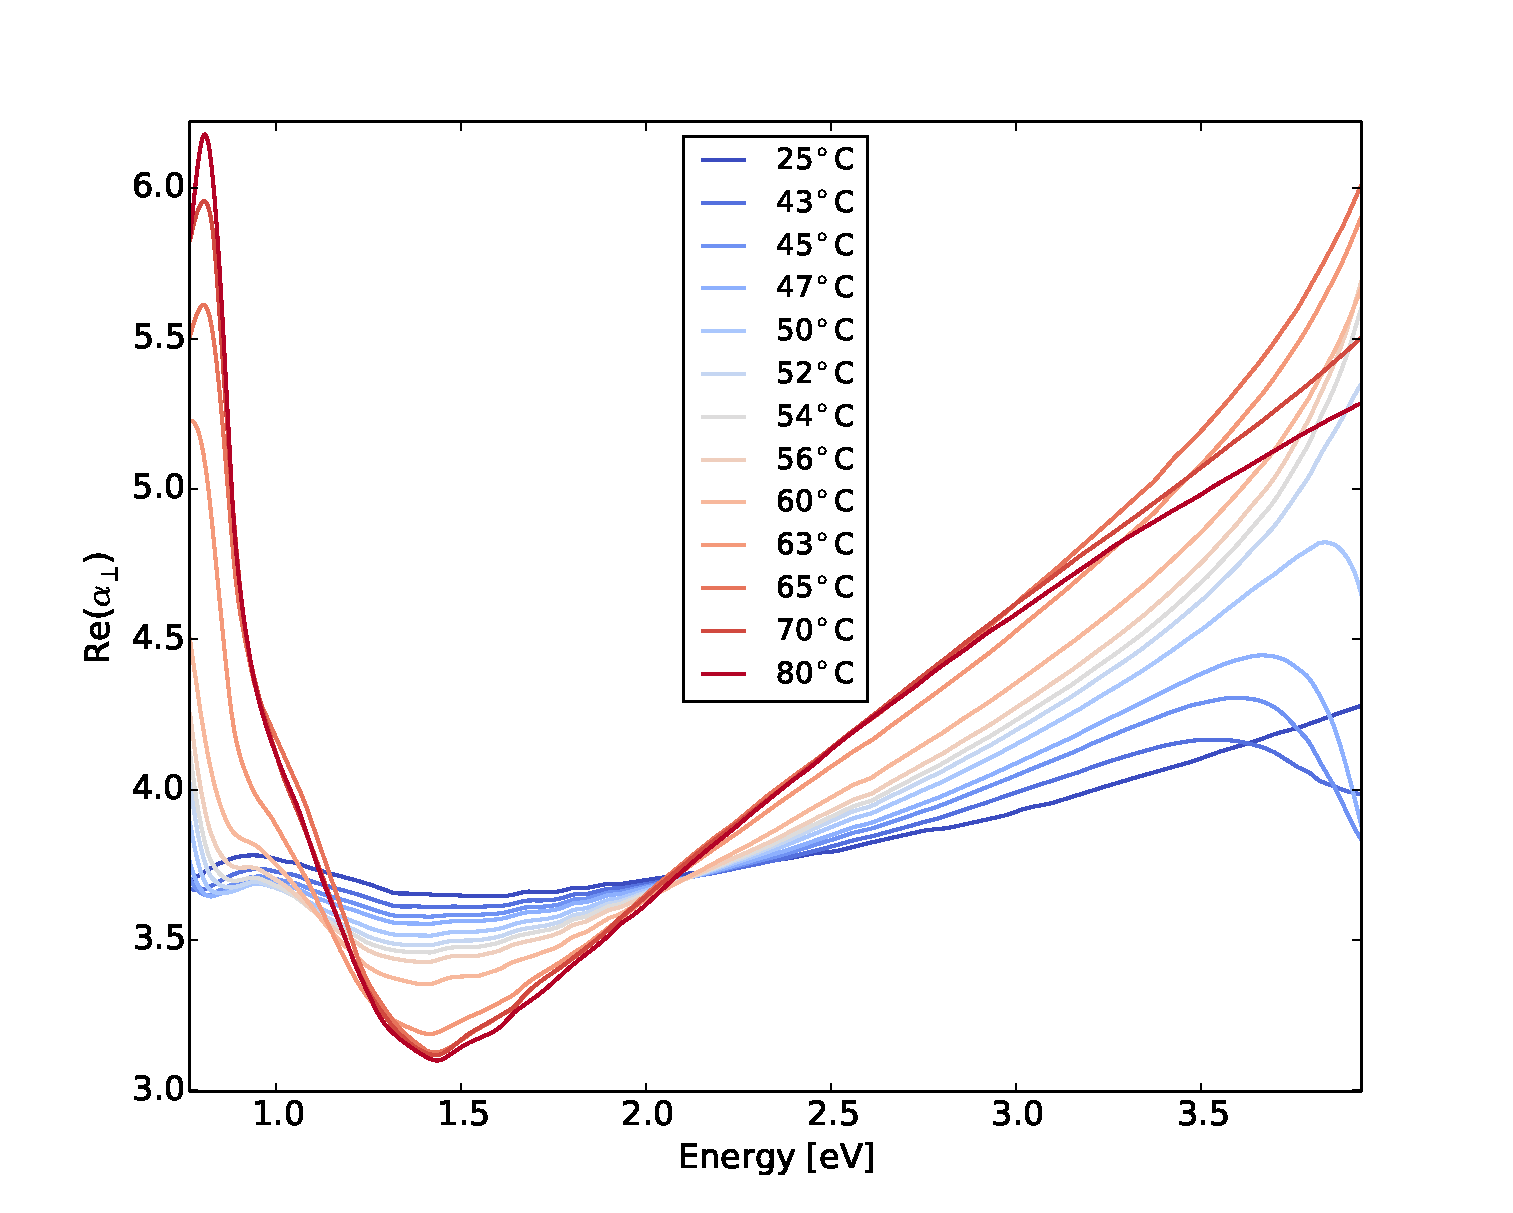
\includegraphics[width=\textwidth]{Results/Sim1/re_alpha_perp.pdf}
        \caption{}
        \label{fig:}
    \end{subfigure}
    %\hfill
    \begin{subfigure}[b]{0.49\textwidth}
        \centering
        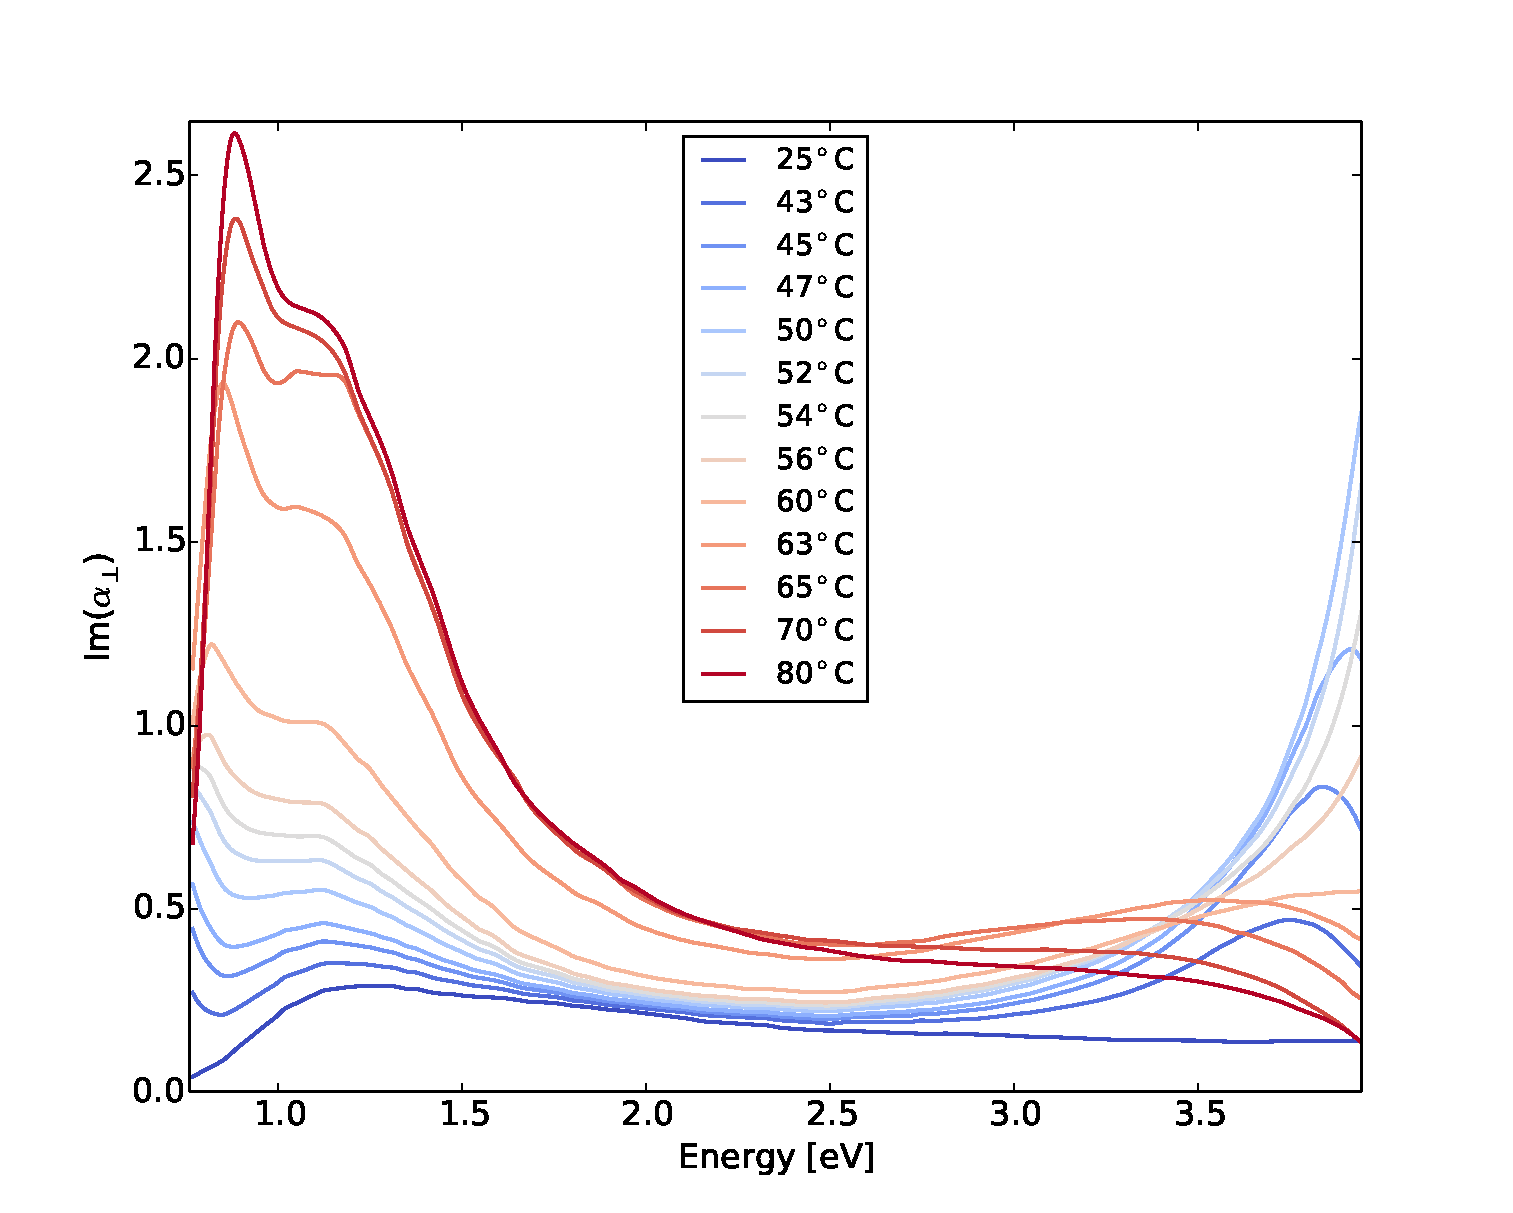
\includegraphics[width=\textwidth]{Results/Sim1/im_alpha_perp.pdf}
        \caption{}
        \label{fig:}
    \end{subfigure}
    %\hfill
    \begin{subfigure}[b]{0.49\textwidth}
        \centering
        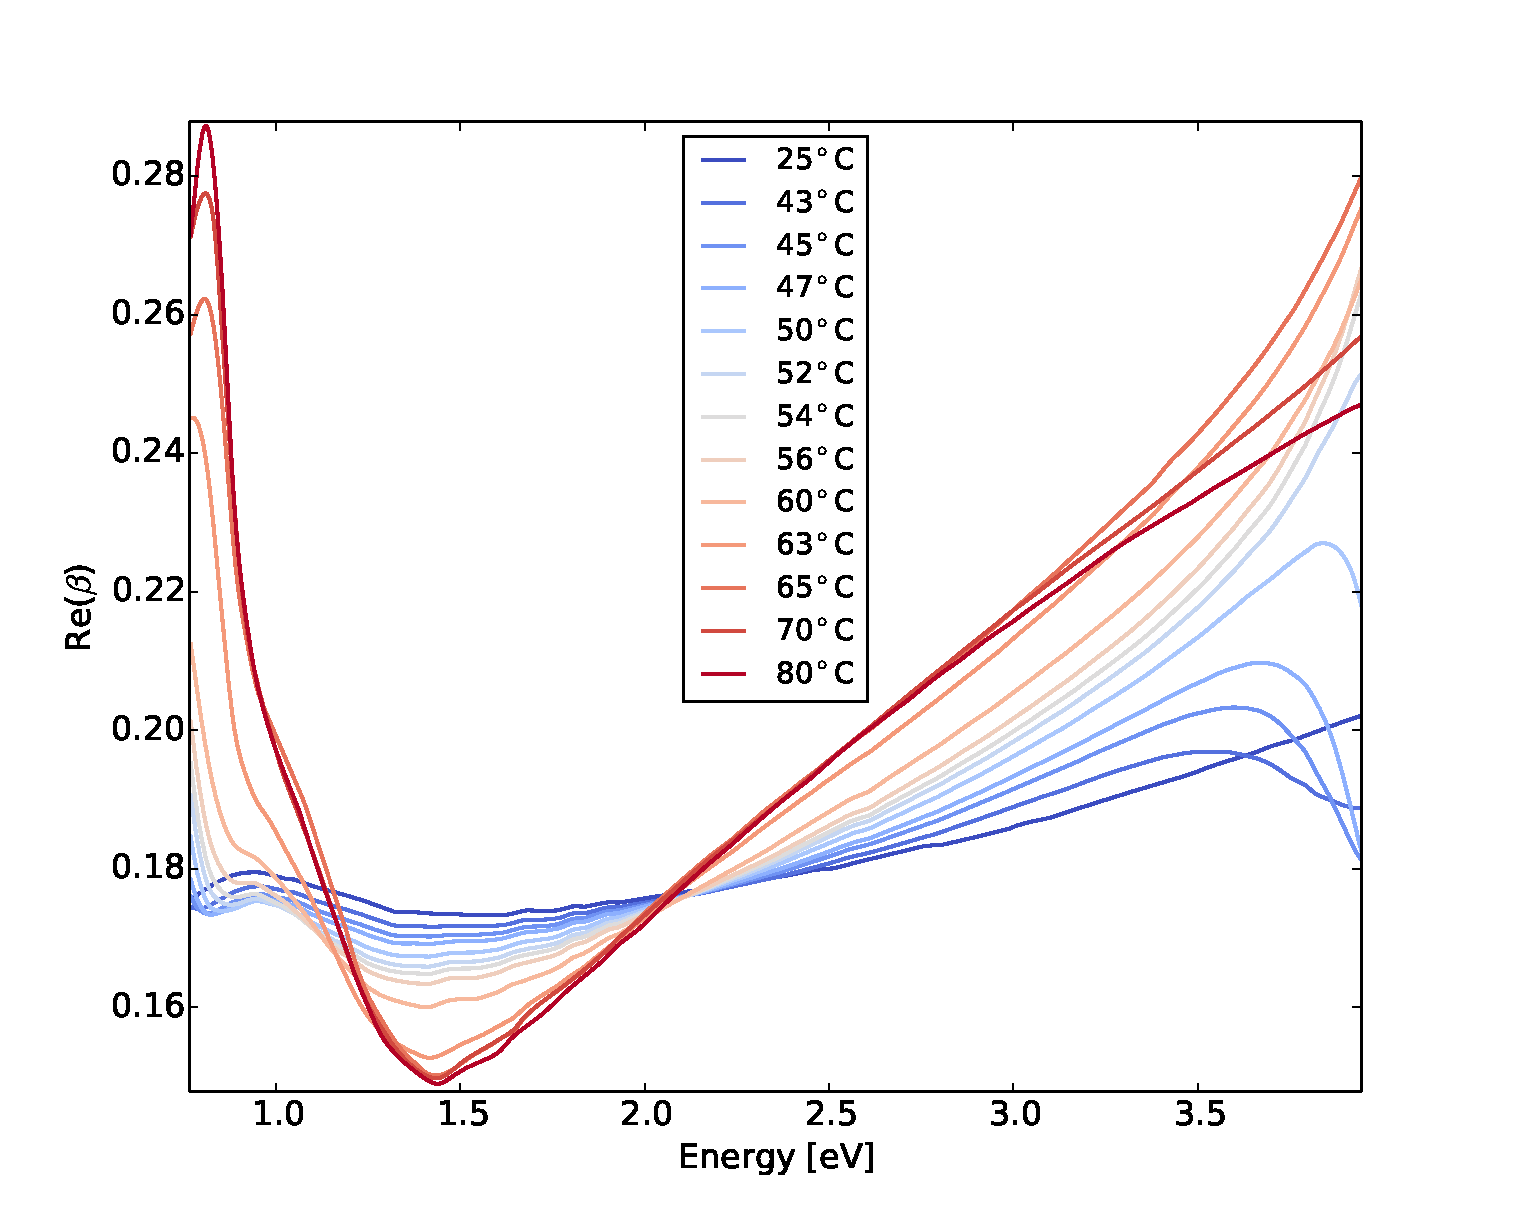
\includegraphics[width=\textwidth]{Results/Sim1/re_beta.pdf}
        \caption{}
        \label{fig:2}
    \end{subfigure}
    %\hfill
    \begin{subfigure}[b]{0.49\textwidth}
        \centering
        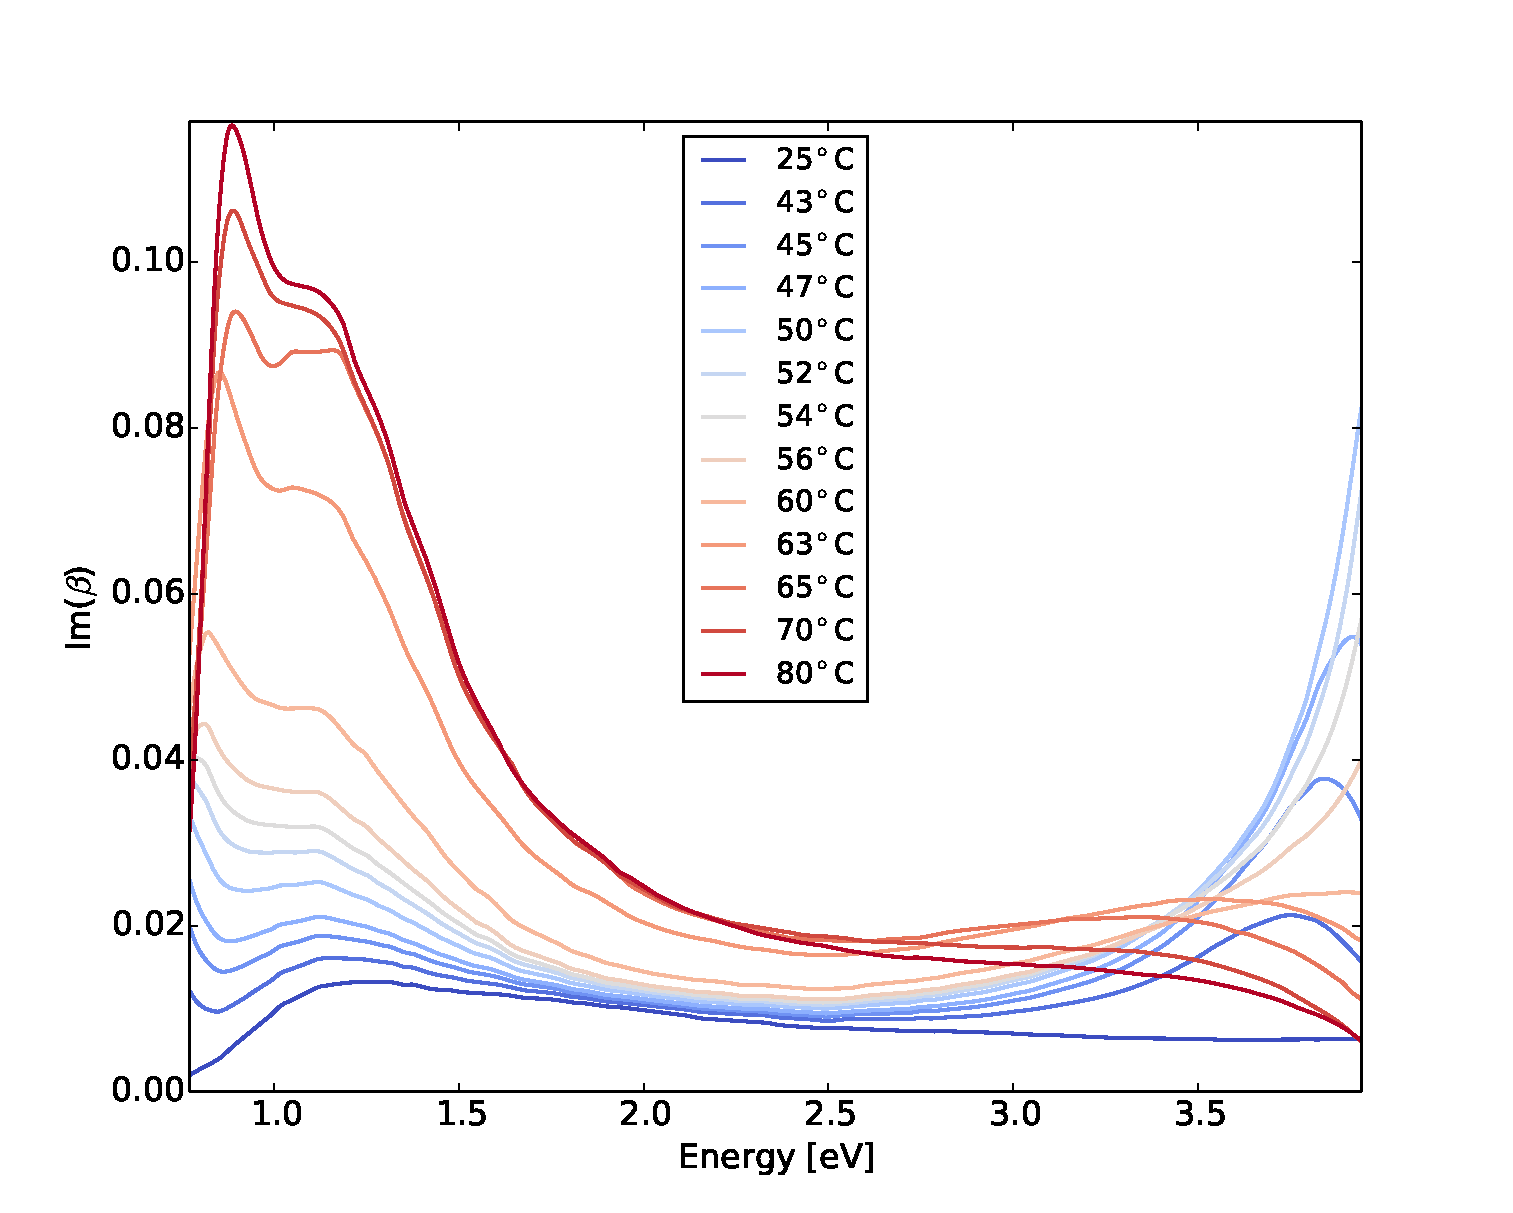
\includegraphics[width=\textwidth]{Results/Sim1/im_beta.pdf}
        \caption{}
        \label{fig:2}
    \end{subfigure}
    \caption{Relative reflectance $\Delta R/R$}
    \label{fig:}
\end{figure}
%


\subsection{Simulation 2; $R = 10$nm, s-polarized incident light}
%
\begin{figure}
    \centering
    \begin{subfigure}[b]{0.49\textwidth}
        \centering
        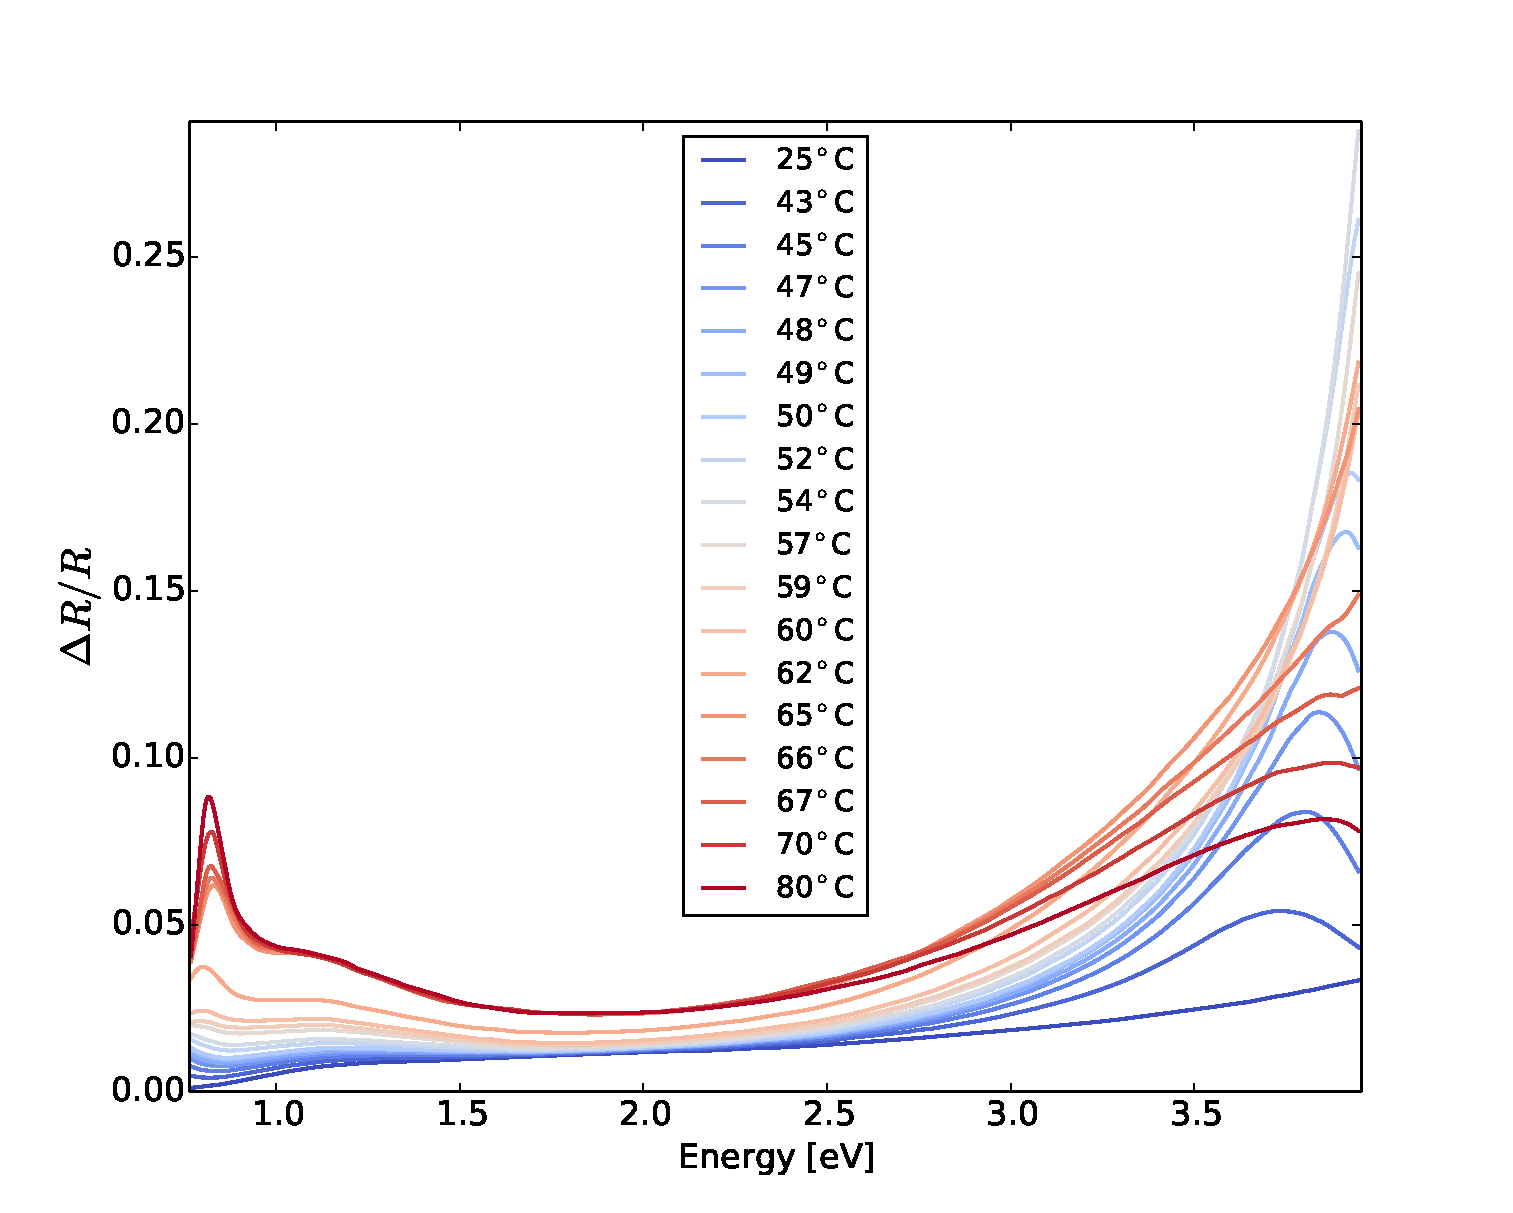
\includegraphics[width=\textwidth]{Results/Sim2/dR.pdf}h
        \caption{}
        \label{fig:}
    \end{subfigure}
    %\hfill
    \begin{subfigure}[b]{0.49\textwidth}
        \centering
        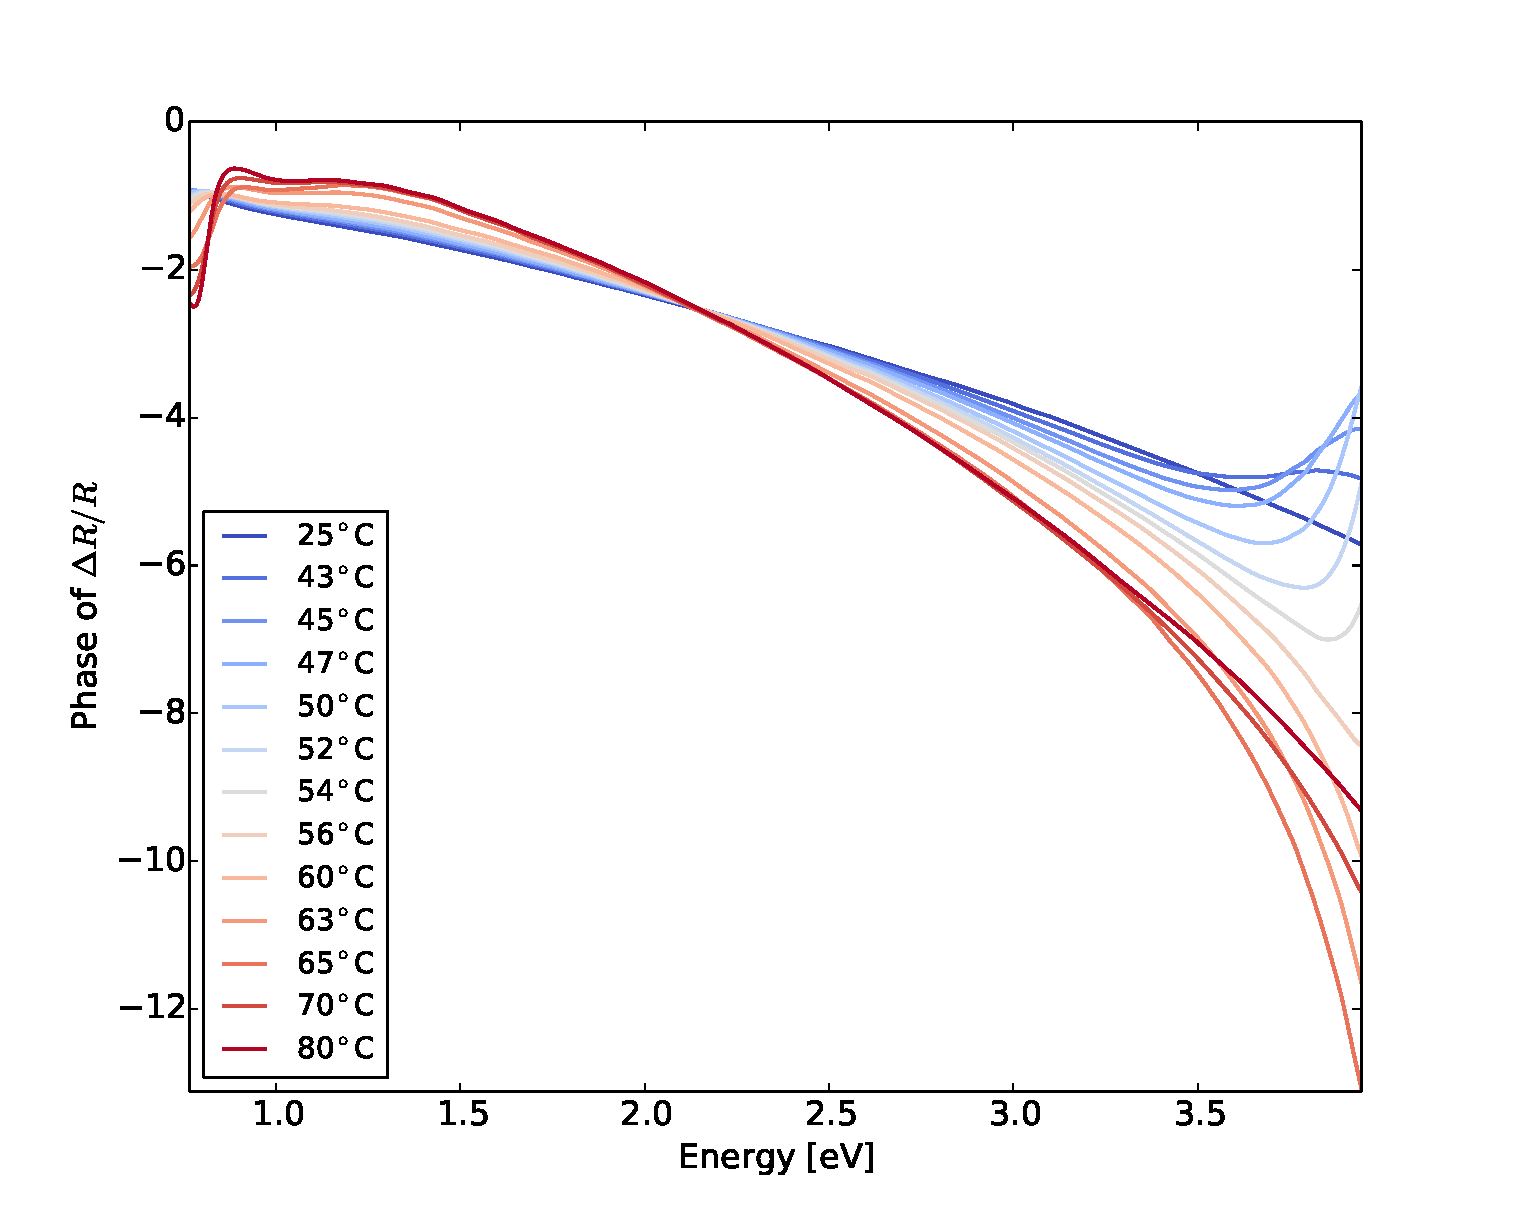
\includegraphics[width=\textwidth]{Results/Sim2/dRphase.pdf}
        \caption{}
        \label{fig:}
    \end{subfigure}
    \caption{Relative reflectance $\Delta R/R$}
    \label{fig:1}
\end{figure}
%
%
\begin{figure}
    \centering
    \begin{subfigure}[b]{0.49\textwidth}
        \centering
        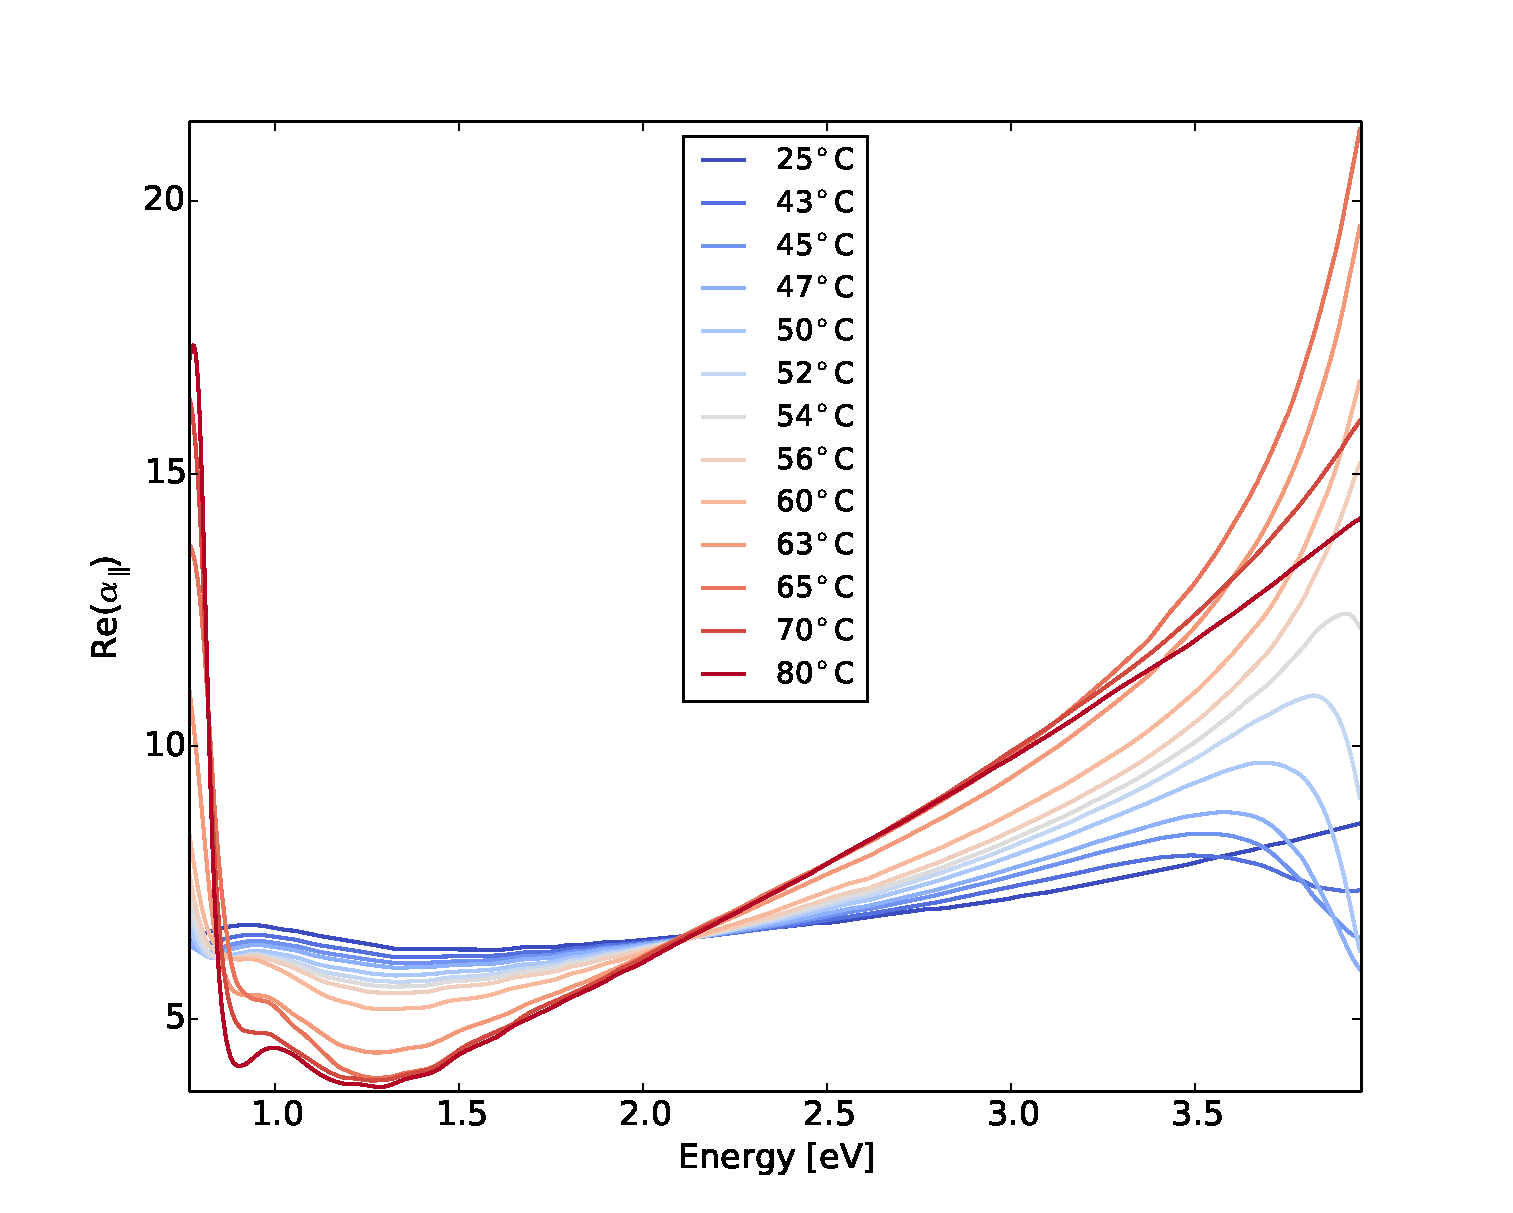
\includegraphics[width=\textwidth]{Results/Sim2/re_alpha_parallel.pdf}
        \caption{}
        \label{fig:2}
    \end{subfigure}
    %\hfill
    \begin{subfigure}[b]{0.49\textwidth}
        \centering
        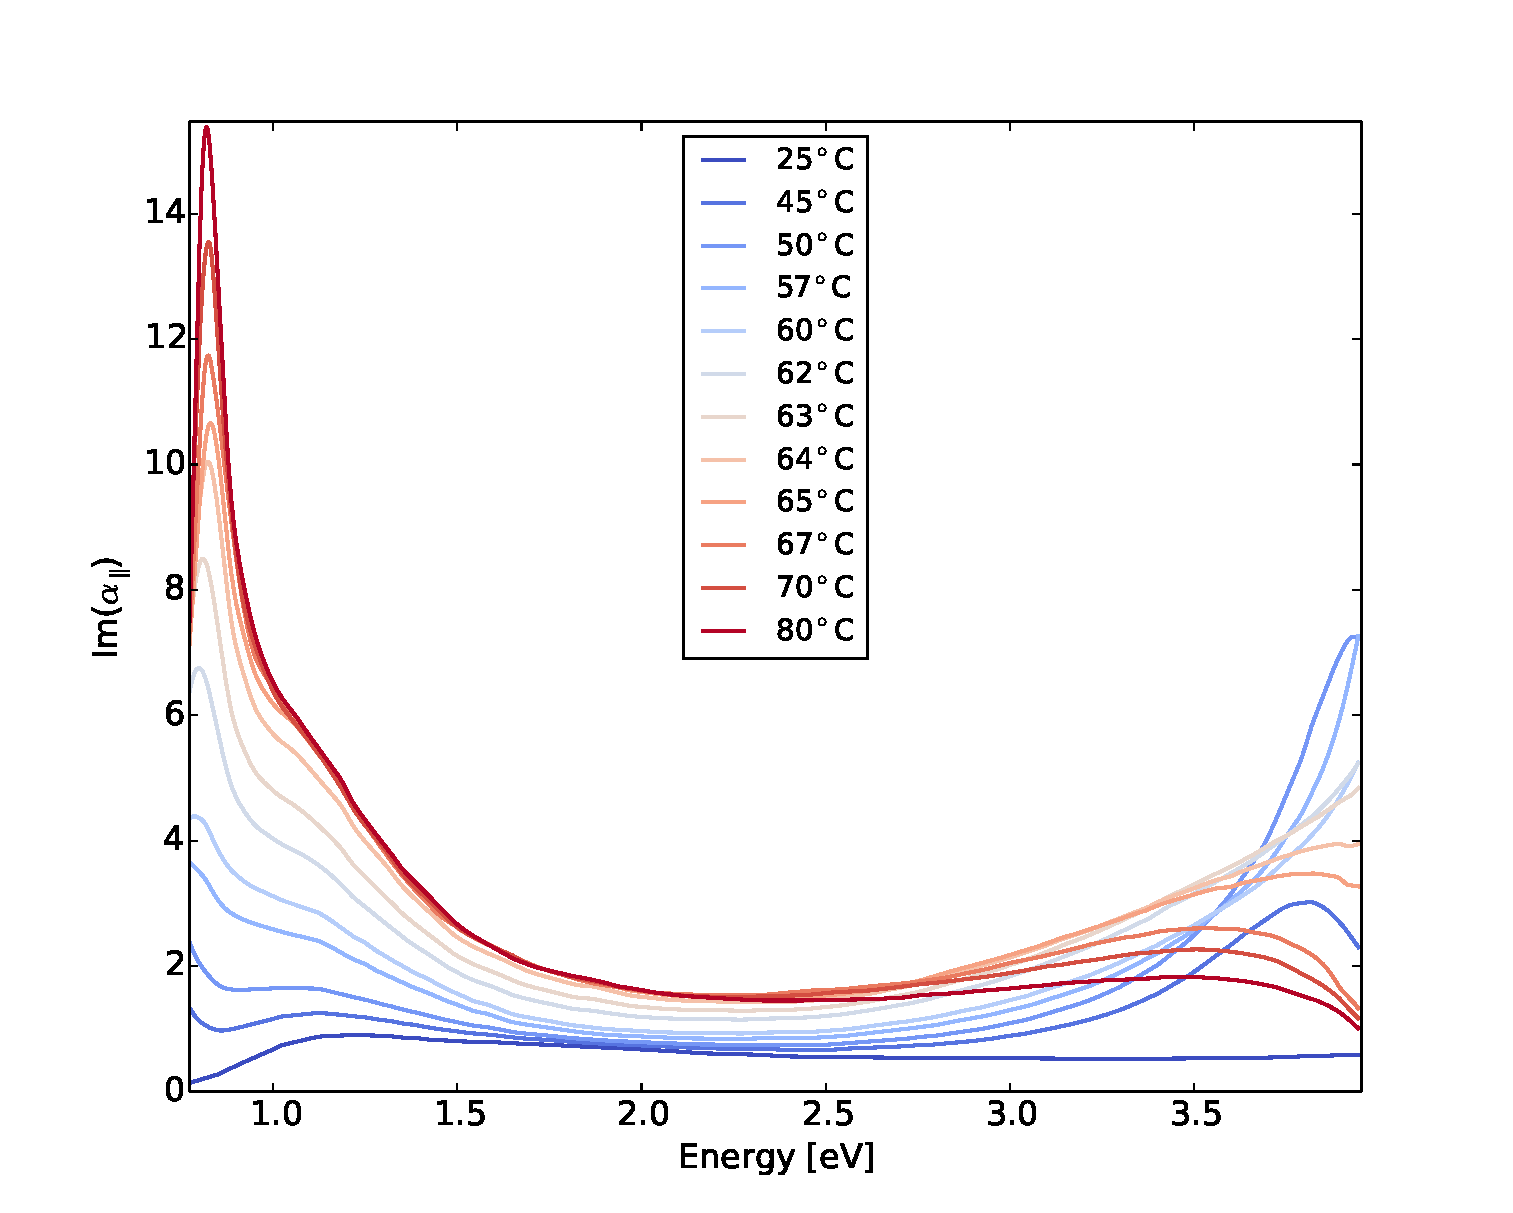
\includegraphics[width=\textwidth]{Results/Sim2/im_alpha_parallel.pdf}
        \caption{}
        \label{fig:2}
    \end{subfigure}
    %\hfill
    \begin{subfigure}[b]{0.49\textwidth}
        \centering
        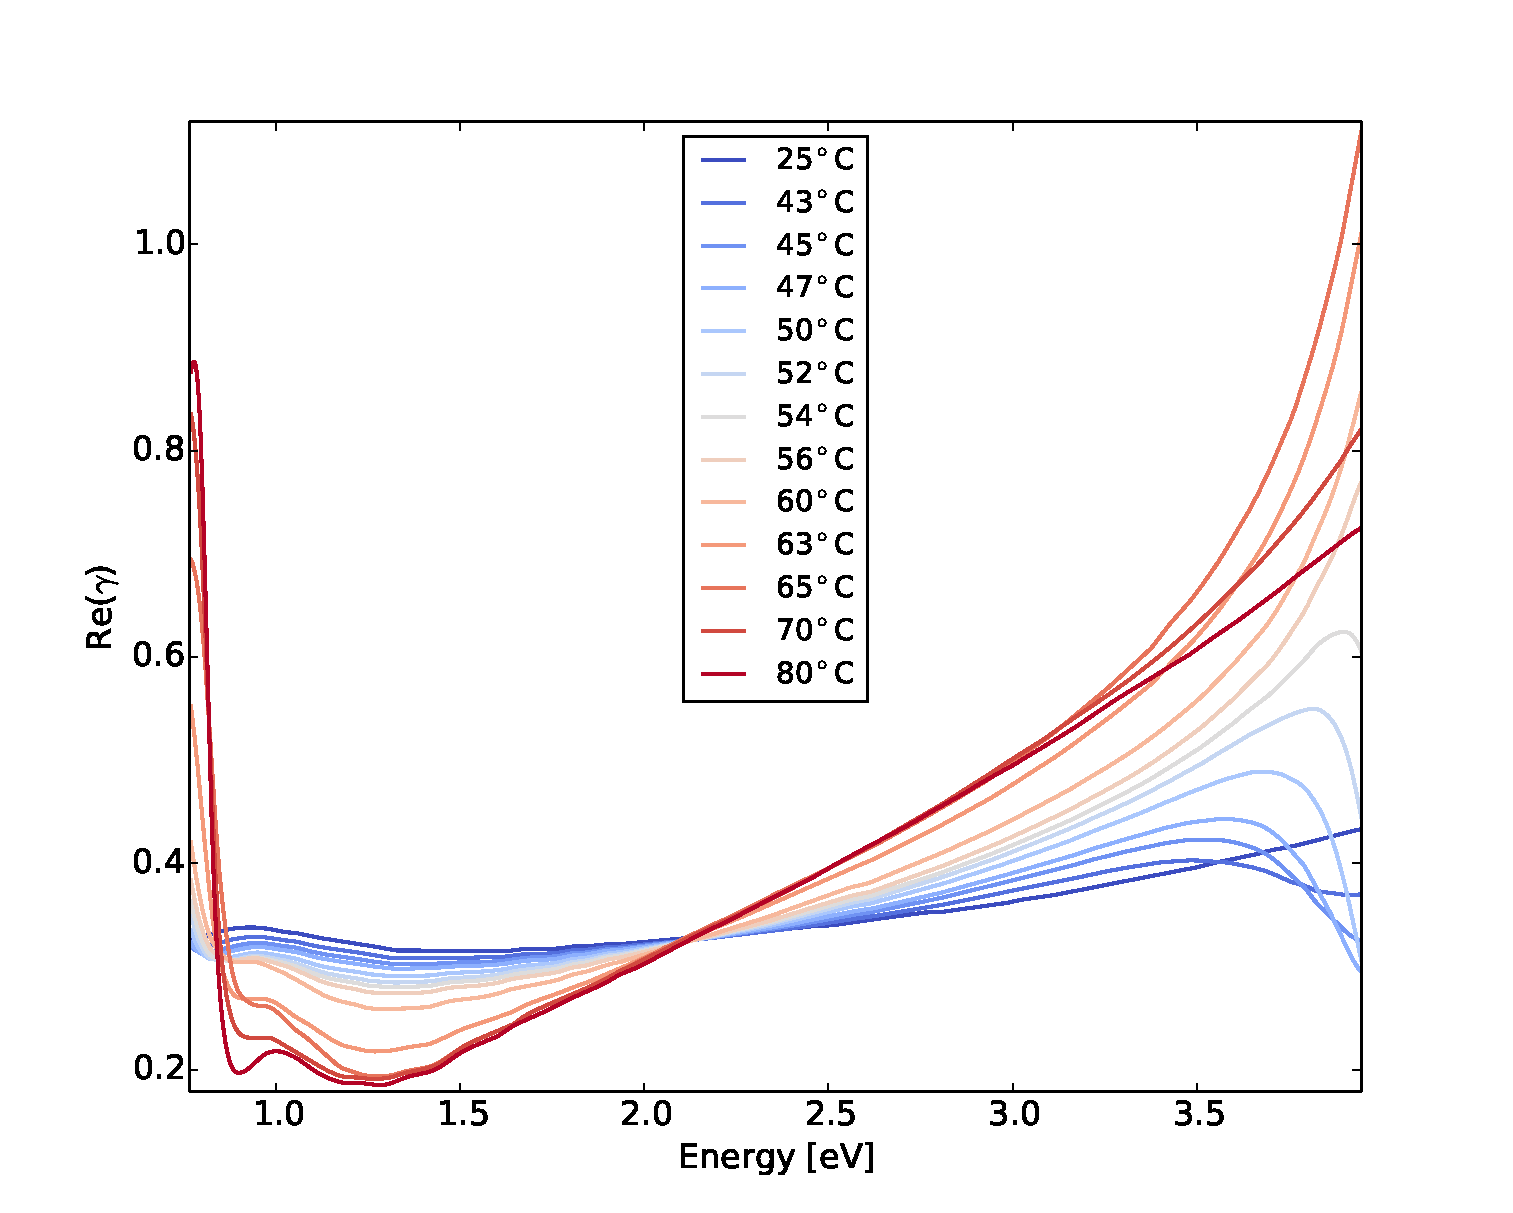
\includegraphics[width=\textwidth]{Results/Sim2/re_gamma.pdf}
        \caption{}
        \label{fig:2}
    \end{subfigure}
    %\hfill
    \begin{subfigure}[b]{0.49\textwidth}
        \centering
        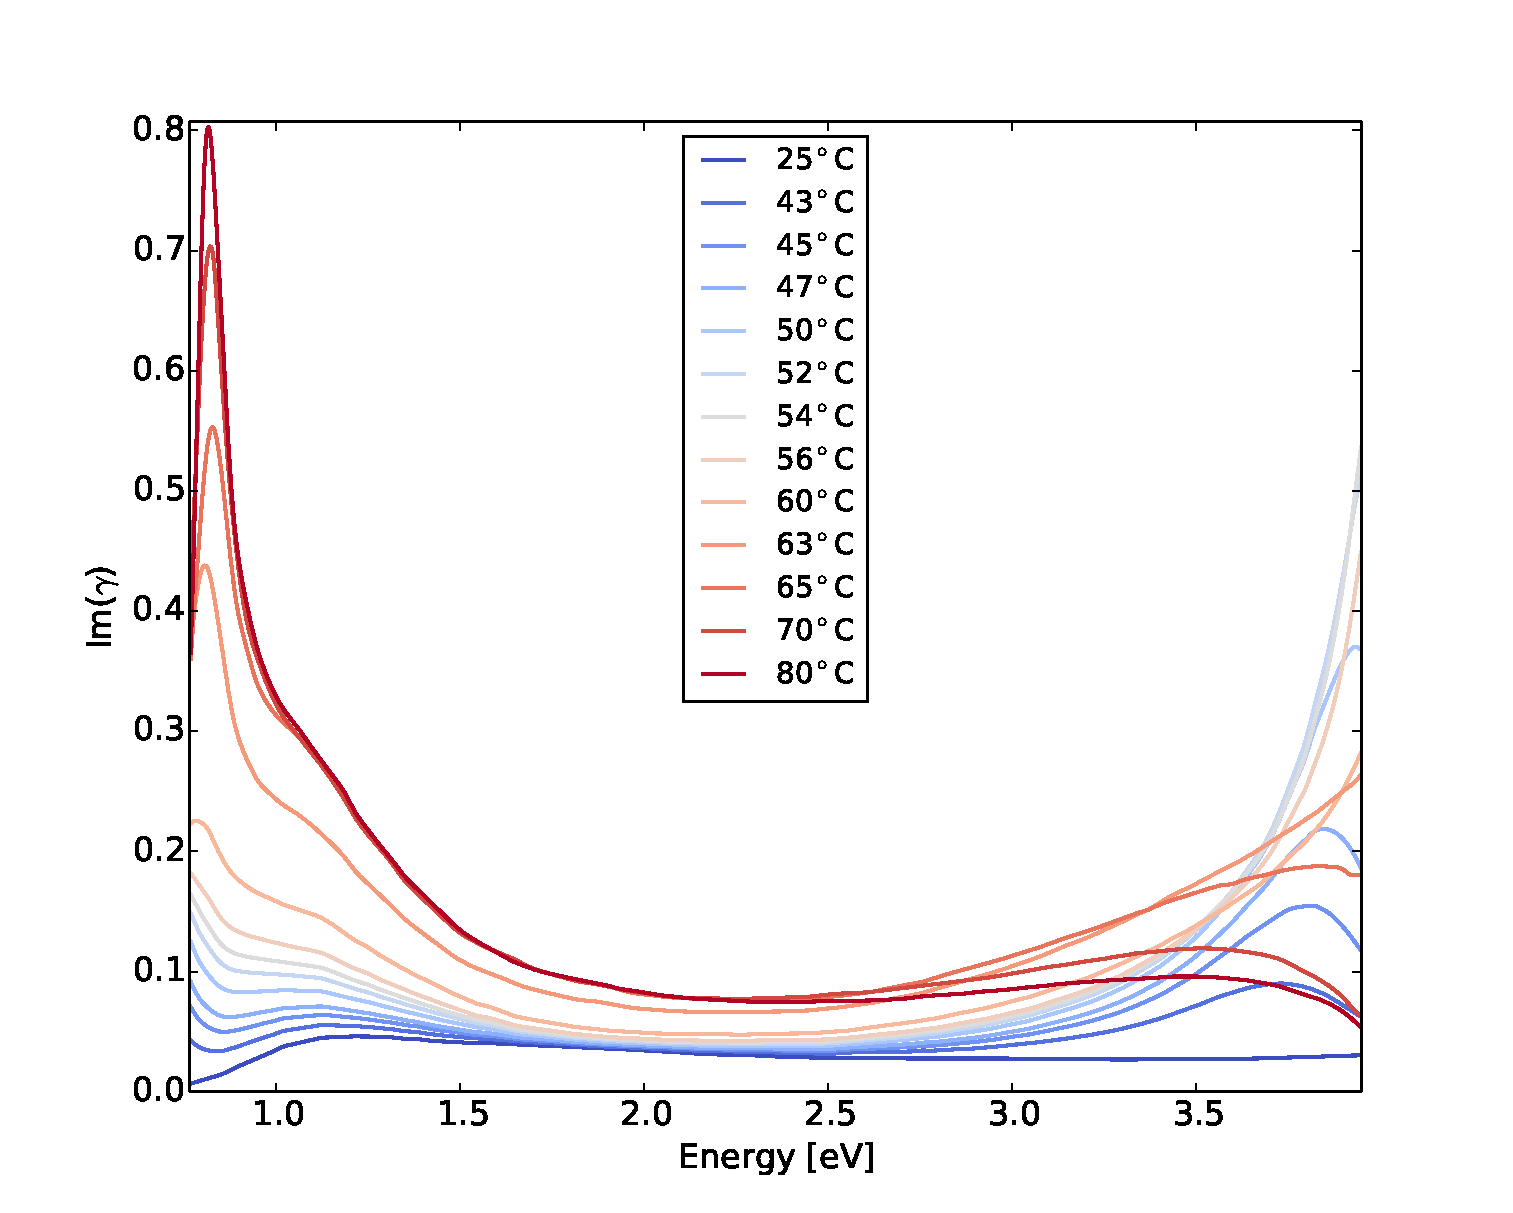
\includegraphics[width=\textwidth]{Results/Sim2/im_gamma.pdf}
        \caption{}
        \label{fig:2}
    \end{subfigure}
    \caption{Relative reflectance $\Delta R/R$}
    \label{fig:}
\end{figure}
%
%
\begin{figure}
    \centering
    \begin{subfigure}[b]{0.49\textwidth}
        \centering
        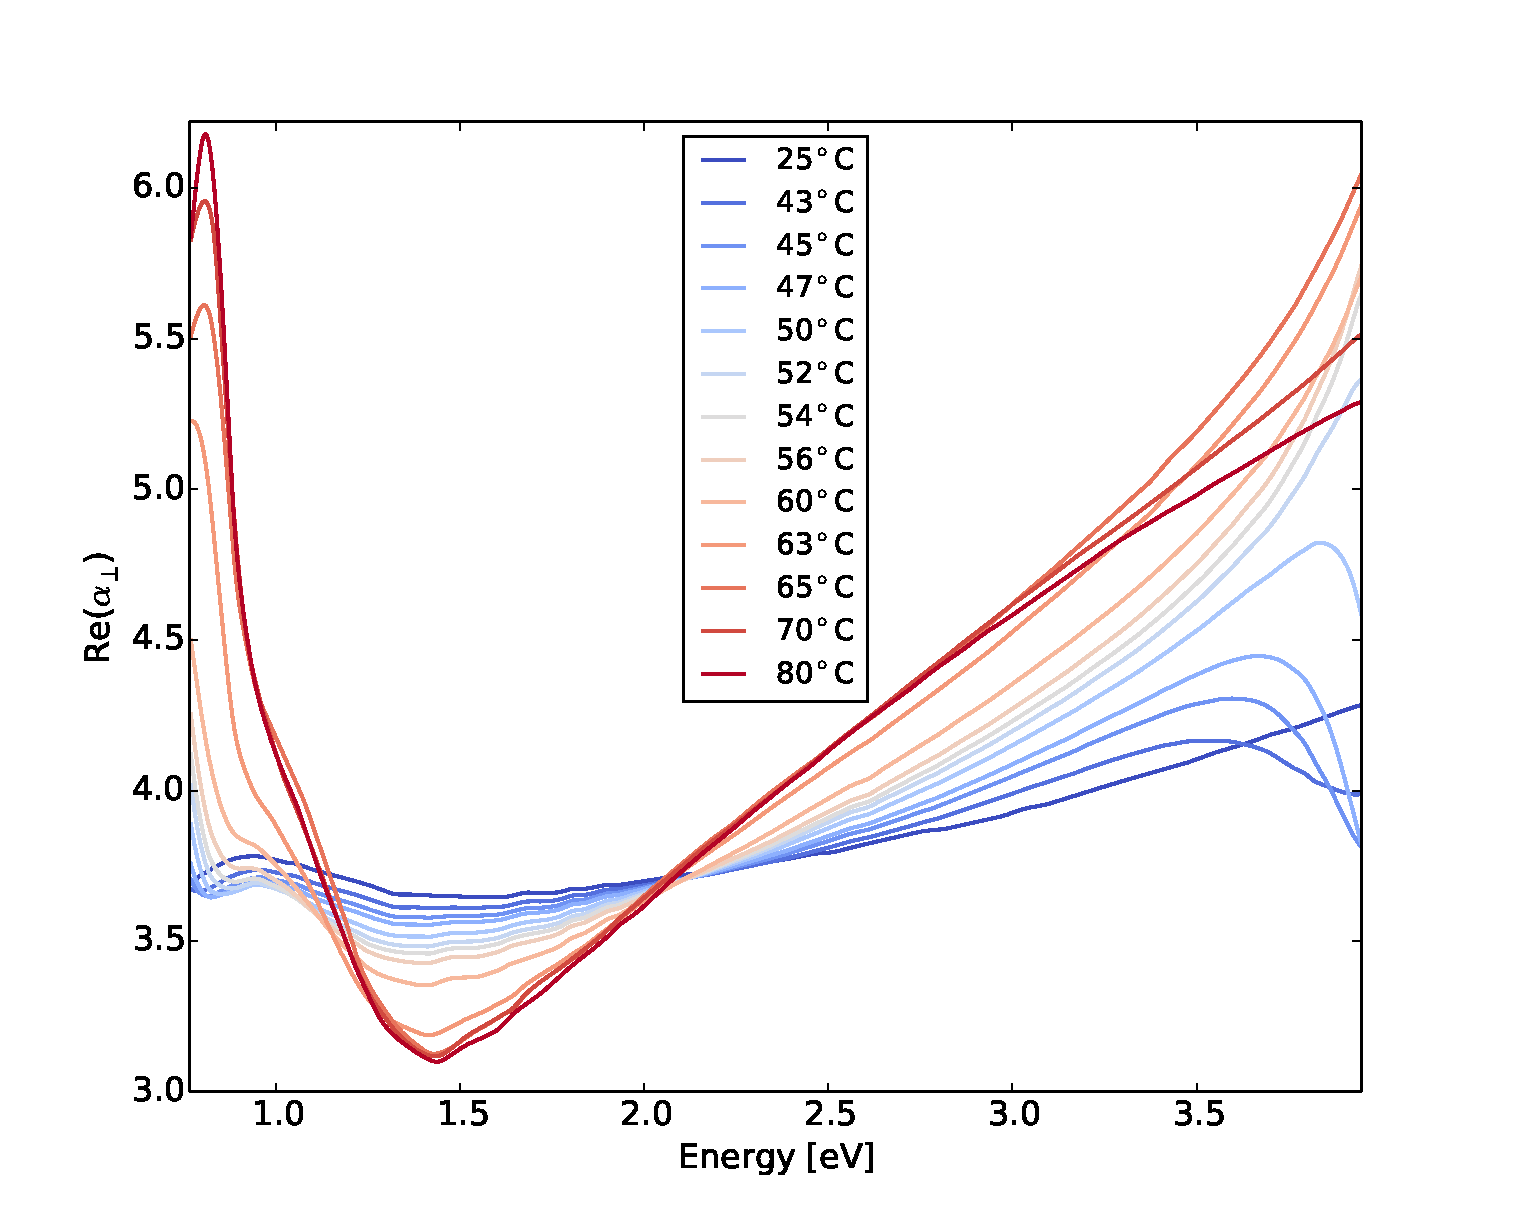
\includegraphics[width=\textwidth]{Results/Sim2/re_alpha_perp.pdf}
        \caption{}
        \label{fig:}
    \end{subfigure}
    %\hfill
    \begin{subfigure}[b]{0.49\textwidth}
        \centering
        \includegraphics[width=\textwidth]{Results/Sim2/im_alpha_perp.pdf}
        \caption{}
        \label{fig:}
    \end{subfigure}
    %\hfill
    \begin{subfigure}[b]{0.49\textwidth}
        \centering
        \includegraphics[width=\textwidth]{Results/Sim2/re_beta.pdf}
        \caption{}
        \label{fig:2}
    \end{subfigure}
    %\hfill
    \begin{subfigure}[b]{0.49\textwidth}
        \centering
        \includegraphics[width=\textwidth]{Results/Sim2/im_beta.pdf}
        \caption{}
        \label{fig:2}
    \end{subfigure}
    \caption{Relative reflectance $\Delta R/R$}
    \label{fig:}
\end{figure}
%



\subsection{Simulation 3; $R = 15$nm, p-polarized incident light}
%
\begin{figure}
    \centering
    \begin{subfigure}[b]{0.49\textwidth}
        \centering
        \includegraphics[width=\textwidth]{Results/Sim3/dR.pdf}
        \caption{}
        \label{fig:}
    \end{subfigure}
    %\hfill
    \begin{subfigure}[b]{0.49\textwidth}
        \centering
        \includegraphics[width=\textwidth]{Results/Sim3/dRphase.pdf}
        \caption{}
        \label{fig:}
    \end{subfigure}
    \caption{Relative reflectance $\Delta R/R$}
    \label{fig:1}
\end{figure}
%
%
\begin{figure}
    \centering
    \begin{subfigure}[b]{0.49\textwidth}
        \centering
        \includegraphics[width=\textwidth]{Results/Sim3/re_alpha_parallel.pdf}
        \caption{}
        \label{fig:2}
    \end{subfigure}
    %\hfill
    \begin{subfigure}[b]{0.49\textwidth}
        \centering
        \includegraphics[width=\textwidth]{Results/Sim3/im_alpha_parallel.pdf}
        \caption{}
        \label{fig:2}
    \end{subfigure}
    %\hfill
    \begin{subfigure}[b]{0.49\textwidth}
        \centering
        \includegraphics[width=\textwidth]{Results/Sim3/re_gamma.pdf}
        \caption{}
        \label{fig:2}
    \end{subfigure}
    %\hfill
    \begin{subfigure}[b]{0.49\textwidth}
        \centering
        \includegraphics[width=\textwidth]{Results/Sim3/im_gamma.pdf}
        \caption{}
        \label{fig:2}
    \end{subfigure}
    \caption{Relative reflectance $\Delta R/R$}
    \label{fig:}
\end{figure}
%
%
\begin{figure}
    \centering
    \begin{subfigure}[b]{0.49\textwidth}
        \centering
        \includegraphics[width=\textwidth]{Results/Sim3/re_alpha_perp.pdf}
        \caption{}
        \label{fig:}
    \end{subfigure}
    %\hfill
    \begin{subfigure}[b]{0.49\textwidth}
        \centering
        \includegraphics[width=\textwidth]{Results/Sim3/im_alpha_perp.pdf}
        \caption{}
        \label{fig:}
    \end{subfigure}
    %\hfill
    \begin{subfigure}[b]{0.49\textwidth}
        \centering
        \includegraphics[width=\textwidth]{Results/Sim3/re_beta.pdf}
        \caption{}
        \label{fig:2}
    \end{subfigure}
    %\hfill
    \begin{subfigure}[b]{0.49\textwidth}
        \centering
        \includegraphics[width=\textwidth]{Results/Sim3/im_beta.pdf}
        \caption{}
        \label{fig:2}
    \end{subfigure}
    \caption{Relative reflectance $\Delta R/R$}
    \label{fig:}
\end{figure}
%

\subsection{Simulation 4; $R = 15$nm, s-polarized incident light}
%
\begin{figure}
    \centering
    \begin{subfigure}[b]{0.49\textwidth}
        \centering
        \includegraphics[width=\textwidth]{Results/Sim4/dR.pdf}
        \caption{}
        \label{fig:}
    \end{subfigure}
    %\hfill
    \begin{subfigure}[b]{0.49\textwidth}
        \centering
        \includegraphics[width=\textwidth]{Results/Sim4/dRphase.pdf}
        \caption{}
        \label{fig:}
    \end{subfigure}
    \caption{Relative reflectance $\Delta R/R$}
    \label{fig:1}
\end{figure}
%
%
\begin{figure}
    \centering
    \begin{subfigure}[b]{0.49\textwidth}
        \centering
        \includegraphics[width=\textwidth]{Results/Sim4/re_alpha_parallel.pdf}
        \caption{}
        \label{fig:2}
    \end{subfigure}
    %\hfill
    \begin{subfigure}[b]{0.49\textwidth}
        \centering
        \includegraphics[width=\textwidth]{Results/Sim4/im_alpha_parallel.pdf}
        \caption{}
        \label{fig:2}
    \end{subfigure}
    %\hfill
    \begin{subfigure}[b]{0.49\textwidth}
        \centering
        \includegraphics[width=\textwidth]{Results/Sim4/re_gamma.pdf}
        \caption{}
        \label{fig:2}
    \end{subfigure}
    %\hfill
    \begin{subfigure}[b]{0.49\textwidth}
        \centering
        \includegraphics[width=\textwidth]{Results/Sim4/im_gamma.pdf}
        \caption{}
        \label{fig:2}
    \end{subfigure}
    \caption{Relative reflectance $\Delta R/R$}
    \label{fig:}
\end{figure}
%
%
\begin{figure}
    \centering
    \begin{subfigure}[b]{0.49\textwidth}
        \centering
        \includegraphics[width=\textwidth]{Results/Sim4/re_alpha_perp.pdf}
        \caption{}
        \label{fig:}
    \end{subfigure}
    %\hfill
    \begin{subfigure}[b]{0.49\textwidth}
        \centering
        \includegraphics[width=\textwidth]{Results/Sim4/im_alpha_perp.pdf}
        \caption{}
        \label{fig:}
    \end{subfigure}
    %\hfill
    \begin{subfigure}[b]{0.49\textwidth}
        \centering
        \includegraphics[width=\textwidth]{Results/Sim4/re_beta.pdf}
        \caption{}
        \label{fig:2}
    \end{subfigure}
    %\hfill
    \begin{subfigure}[b]{0.49\textwidth}
        \centering
        \includegraphics[width=\textwidth]{Results/Sim4/im_beta.pdf}
        \caption{}
        \label{fig:2}
    \end{subfigure}
    \caption{Relative reflectance $\Delta R/R$}
    \label{fig:}
\end{figure}
%




\begin{figure}
    \centering
    \begin{subfigure}[b]{0.3\textwidth}
        \centering
        \includegraphics[width=\textwidth]{Results/Sim1/dR_visible.pdf}
        \caption{}
        %\label{fig:y equals x}
    \end{subfigure}
    %\hfill
    \begin{subfigure}[b]{0.3\textwidth}
        \centering
        \includegraphics[width=\textwidth]{Results/Sim1/dRphase_visible.pdf}
        \caption{}
        %\label{fig:five over x}
    \end{subfigure}
    %\hfill
    \begin{subfigure}[b]{0.3\textwidth}
        \centering
        \includegraphics[width=\textwidth]{Results/Sim1/dRphase_visible_log.pdf}
        \caption{}
        %\label{fig:three sin x}
    \end{subfigure}
    \caption{R = 10nm, p-pol}
    %\label{fig:three graphs}
\end{figure}
%
\begin{figure}
    \centering
    \begin{subfigure}[b]{0.3\textwidth}
        \centering
        \includegraphics[width=\textwidth]{Results/Sim2/dR_visible.pdf}
        \caption{}
        %\label{fig:y equals x}
    \end{subfigure}
    %\hfill
    \begin{subfigure}[b]{0.3\textwidth}
        \centering
        \includegraphics[width=\textwidth]{Results/Sim2/dRphase_visible.pdf}
        \caption{}
        %\label{fig:five over x}
    \end{subfigure}
    %\hfill
    \begin{subfigure}[b]{0.3\textwidth}
        \centering
        \includegraphics[width=\textwidth]{Results/Sim2/dRphase_visible_log.pdf}
        \caption{}
        %\label{fig:three sin x}
    \end{subfigure}
    \caption{R = 10nm, s-pol}
    %\label{fig:three graphs}
\end{figure}
%
\begin{figure}
    \centering
    \begin{subfigure}[b]{0.3\textwidth}
        \centering
        \includegraphics[width=\textwidth]{Results/Sim3/dR_visible.pdf}
        \caption{}
        %\label{fig:y equals x}
    \end{subfigure}
    %\hfill
    \begin{subfigure}[b]{0.3\textwidth}
        \centering
        \includegraphics[width=\textwidth]{Results/Sim3/dRphase_visible.pdf}
        \caption{}
        %\label{fig:five over x}
    \end{subfigure}
    %\hfill
    \begin{subfigure}[b]{0.3\textwidth}
        \centering
        \includegraphics[width=\textwidth]{Results/Sim3/dRphase_visible_log.pdf}
        \caption{}
        %\label{fig:three sin x}
    \end{subfigure}
    \caption{R = 15nm, p-pol}
    %\label{fig:three graphs}
\end{figure}
%
\begin{figure}
    \centering
    \begin{subfigure}[b]{0.3\textwidth}
        \centering
        \includegraphics[width=\textwidth]{Results/Sim4/dR_visible.pdf}
        \caption{}
        %\label{fig:y equals x}
    \end{subfigure}
    %\hfill
    \begin{subfigure}[b]{0.3\textwidth}
        \centering
        \includegraphics[width=\textwidth]{Results/Sim4/dRphase_visible.pdf}
        \caption{}
        %\label{fig:five over x}
    \end{subfigure}
    %\hfill
    \begin{subfigure}[b]{0.3\textwidth}
        \centering
        \includegraphics[width=\textwidth]{Results/Sim4/dRphase_visible_log.pdf}
        \caption{}
        %\label{fig:three sin x}
    \end{subfigure}
    \caption{R = 15nm, s-pol}
    %\label{fig:three graphs}
\end{figure}
%


\newpage

\section{Discussion}

%\section{Conclusion}


%\section{Introduction to GranFilm}
This section is included as a brief summary of the practical situations one encounter
when using GranFilm. Even though the software provides the information required and would be
self-explanatory for some, this would be for the less experienced reader to avoid any unecessary 
confusion.

\subsection{Software overview}
\textsc{GranFilm} is a program written in \textsc{Fortran 90} and serves as a tool for simulating 
and interpreting optical spectra from surfaces or thin films. The program takes in parameters specifying
the incoming angle, polarization and energy range of the incoming plane wave, in addition to the
radius and truncation ratio $t_r$ of the sphere, the materials for region 1,2,3 and 4,
the arrangement of the islands and finally the multipole order $M$.  




\newpage
%\clearpage
\begin{thebibliography}{9}

%		\bibitem{poisson}
%		Einar M. Rønquist,
%		\emph{The Poisson problem in $\mathbb{R}^2$: Diagonalization methods},
%		Department of Mathematical Sciences,
%		NTNU,N-7491 Trondheim, Norway,
%		Revised by Arne Morten Kvarving, 2014.

      \bibitem{opticalProperties}
      D. Bedeaux, J. Vlieger, 
      \emph{Optical Properties of Surfaces}, 
      Imperial College Press, 
      London, 2001

      %\bibitem{griffiths}
      %D. J. Griffiths.
      %\emph{Introduction To Electrodynamics}.
      %???Prentice Hall, Third Edition, 2004. ???

\end{thebibliography}



%
\end{document}

